\documentclass{book}
\usepackage{CJKutf8}
\usepackage{amsmath}
\usepackage{amsfonts}
\usepackage{amsthm}
\usepackage{titlesec}
\usepackage{titletoc}
\usepackage{xCJKnumb}
\usepackage{tikz}
\titleformat{\chapter}{\centering\Huge\bfseries}{第\, \xCJKnumber{\thechapter}\,
    章}{1em}{}
  % \renewcommand{\chaptermark}[1]{\markboth{第 \thechapter 章}{}}

\newtheorem{Def}{定义}[chapter]
\newtheorem{Ex}{习题}[chapter]


\begin{document}
\begin{CJK*}{UTF8}{gbsn}
  \title{离散数学}
  \author{陈建文}
  \maketitle
  %\tableofcontents
  

  \chapter{集合}
\begin{Ex}[课本第8页第3题]
  \mbox{} \par \noindent
  
写出方程
\begin{equation*}
x^2+2x+1=0
\end{equation*}
的根构成的集合。
\end{Ex}

  \chapter{映射}

  \begin{Def}
    设$X$和$Y$为两个非空集合。一个从$X$到$Y$的映射$f$为一个法则,根据$f$,对$X$中的每个元素$x$都有$Y$中唯一确定的元素$y$与之对应。
    从$X$到$Y$的映射$f$常记为$f:X\to Y$。
  \end{Def}

  \begin{Example}
    设集合$X=\{-1,0,1\}$,集合$Y=\{0,1,2\}$,$\forall x \in X, f(x)=x^2$,即$f(-1)=1,f(0)=0,f(1)=1$,则$f$为从集合$X$到集合$Y$的映射。
  \end{Example}

  \begin{Def}
    设$X$和$Y$为两个非空集合。一个从$X$到$Y$的映射为一个满足以下两个条件的$X\times Y$的子集$f$:
    \begin{enumerate}
    \item 对$X$的每一个元素$x$,存在一个$y\in Y$,使得$(x,y) \in f$;
    \item 若$(x,y)\in f$,$(x,y')\in f$,则$y=y'$。
    \end{enumerate}
    $(x,y)\in f$记为$y=f(x)$。
  \end{Def}
  \begin{Example}
    设集合$X=\{-1,0,1\}$,集合$Y=\{0,1,2\}$,$f=\{(-1,1),(0,0),(1,1)\}$,则$f$为从集合$X$到集合$Y$的映射。
  \end{Example}

  定义2.1和定义2.2是等价的。
  \begin{Def}
    设$f$为从集合$X$到集合$Y$的映射,$f:X\to Y$, 如果$y = f(x)$,则称$y$为$x$在$f$下的象,称$x$为$y$的原象。$X$称为$f$的定义域;集合$\{f(x) | x \in X\}$称为$f$的值域,记为$Im(f)$。
  \end{Def}
  \begin{Def}
    设$f:X\to Y$,$A\subseteq X$,当把$f$的定义域限制在$A$上时,就得到了一个
    $\phi: A\to Y$,$\forall x \in A$,$\phi(x) = f(x)$。$\phi$称为$f$在$A$上的
    限制,并且常用$f|A$来表示$\phi$。反过来,我们也称$f$为$\phi$在$X$上的扩张。
  \end{Def}
    \begin{Def}
    设$f:A \to Y$,$A \subseteq X$, 则称$f$为$X$上的一个部分映射。
  \end{Def}
  \begin{Def}
    两个映射$f$与$g$称为是相等的当且仅当$f$和$g$都为从$X$到$Y$的映射,并且$\forall x \in X$总有$f(x) = g(x)$。
  \end{Def}
  \begin{Def}
    设$f:X\to X$,如果$\forall x \in X, f(x) = x$,则称$f$为$X$上的恒等映射。$X$上的恒等映射常记为$I_X$。
  \end{Def}

    \begin{Def}
    设$f:X\to Y$,如果$\forall x_1, x_2 \in X$, 只要$x_1 \neq x_2$,  就 有 $f(x_1) \neq f(x_2)$,   则称$f$为从$X$到$Y$的单射。
  \end{Def}
  \begin{Def}
    设$f:X\to Y$, 如果$\forall y \in Y$, $\exists x \in X$使得 $f(x) = y$, 则称$f$为从$X$到$Y$的满射。
  \end{Def}
  \begin{Def}
    设$f:X\to Y$,如果$f$既是单射又是满射,则称$f$为从$X$到$Y$的双射,或者称$f$为从$X$到$Y$的一一对应。
  \end{Def}
  \begin{Def}
    设$f:X\to Y$,$A \subseteq X$,$A$在$f$下的象定义为\[f(A)=\{f(x)|x\in A\}\]
  \end{Def}
  \begin{Example}
    设$f:\{-1,0,1\}\to \{-1,0,1\}$,$f(x)=x^2$,则$f(\{-1,0\})=\{0,1\}$
  \end{Example}
  \begin{Def}
    设$f:X\to Y$,$B \subseteq Y$,$B$在$f$下的原象定义为\[f^{-1}(B)=\{x\in X|f(x)\in B\}\]
  \end{Def}
  \begin{Example}
    设$f:\{-1,0,1\}\to \{-1,0,1\}$,$f(x)=x^2$,则$f^{-1}(\{-1,0\})=\{0\}$
  \end{Example}
  \begin{Thm}
    设$f:X\to Y$,$A \subseteq Y$,$B \subseteq Y$, 则
    \begin{enumerate}
    \item $f^{-1}(A \cup B) = f^{-1}(A) \cup f^{-1}(B)$
    \item $f^{-1}(A \cap B) = f^{-1}(A) \cap f^{-1}(B)$
    \item $f^{-1}(A^c)=(f^{-1}(A))^c$
    \item $f^{-1}(A \bigtriangleup B) = f^{-1}(A) \bigtriangleup f^{-1}(B)$
    \end{enumerate}
  \end{Thm}
    \begin{Thm}
    设$f:X\to Y$,$A \subseteq X$,$B \subseteq X$, 则
    \begin{enumerate}
    \item $f(A \cup B) = f(A) \cup f(B)$
    \item $f(A \cap B) \subseteq f(A) \cap f(B)$
    \item $f(A \bigtriangleup B) \supseteq f(A) \bigtriangleup f(B)$
    \end{enumerate}
  \end{Thm}

  \begin{Def}
    设$f:X\to Y$,$g:Y\to Z$为映射,映射$f$与$g$的合成$g\circ f:X\to Z$定义为\[(g\circ f)(x) = g(f(x))\]
  \end{Def}
\begin{Thm}
  设$f:X \to Y$,$g:Y\to Z$,$h:Z\to W$ 为映射,则 \[ (h \circ g) \circ f = h \circ (g \circ f) \]
\end{Thm}

  \begin{Def}
     设$f:X\to Y$为双射,$f$的逆映射$f^{-1}:Y\to X$定义为:对任意的$y\in Y$,存在唯一的$x$使得$f(x)=y$,则$f^{-1}(y)=x$。
   \end{Def}
   \begin{Example}
     设集合$X=\{1,2,3\}$,$Y=\{4,5,6\}$,$f=\{(1,4),(2,5),(3,6)\}$为从$X$到$Y$的双射,则$f^{-1}=\{(4,1),(5,2),(6,3)\}$。
   \end{Example}
    \begin{Def}
     设$f:X\to Y$为一个映射。如果存在一个映射$g:Y\to X$使得\[f\circ g = I_{Y} \text{且} g\circ f = I_{X},\]则称映射$f$为可逆的,而$g$称为$f$的逆映射。
   \end{Def}
      \begin{Example}
     设集合$X=\{1,2,3\}$,$Y=\{4,5,6\}$,$f=\{(1,4),(2,5),(3,6)\}$为从$X$到$Y$的双射,$g=\{(4,1),(5,2),(6,3)\}$,由于$f\circ g = I_{Y}$且$ g\circ f = I_{X}$,$f^{-1}=g$。
   \end{Example}

   以上两个定义是等价的。

     \begin{Thm}
    设$f:X\to Y$为可逆映射,则$(f^{-1})^{-1}=f$。
  \end{Thm}
  \begin{Thm}
    设$f:X\to Y$,$g:Y\to Z$都为可逆映射,则$g\circ f$也为可逆映射并且$(g\circ f)^{-1} = f^{-1}\circ g^{-1}$。
  \end{Thm}

    \begin{Def}
    设$f:X\to Y$为一个映射,如果存在一个映射 $g:Y\to X$ 使 得 $g\circ f = I_X$,
    则称$f$为左可逆的,$g$称为$f$的左逆映射;如果存在一个映射
    $h:Y\to X$ 使 得 $f\circ h=I_Y$,则称$f$为右可逆的,$h$称为$f$的右逆映射。
  \end{Def}
  \begin{Thm}
    设$f:X\to Y$为一个映射,则
    \begin{enumerate}
    \item $f$左可逆当且仅当$f$为单射;
    \item $f$右可逆当且仅当$f$为满射。
    \end{enumerate}
  \end{Thm}

  \begin{Def}
    有穷集合$S$到自身的一一对应称为$S$上的一个置换。如果$|S| = n$, 则$S$上的置换就说成是$n$次置换。
  \end{Def}
设$S=\{1,2,\ldots,n\}$,$\sigma:S\to S$为$S$上的一个置换,$\sigma(1) = k_1$, $\sigma(2) = k_2$,$\ldots$,$\sigma(n) = k_n$,我们用如下的一个表来表示置换$\sigma$:
\[\sigma=\begin{pmatrix}1&2&\ldots&n\\k_1&k_2&\ldots&k_n\end{pmatrix}\]
\begin{Example}
  设$S=\{1,2,3,4\}$,$\sigma(1) = 3$, $\sigma(2) = 2$, $\sigma(3) = 4$, $\sigma(4) = 1$,则$\sigma$可以表示为
  \[\sigma=\begin{pmatrix}1&2&3&4\\3&2&4&1\end{pmatrix}\]
  这里,列的次序无关紧要,例如,$\sigma$还可以表示为
  \[\sigma=\begin{pmatrix}2&1&3&4\\2&3&4&1\end{pmatrix}\]
\end{Example}

  \begin{Def}
    设$\alpha$与$\beta$为集合$S=\{1,2,3,4\}$上的两个置换,则$\alpha$与$\beta$为两个从$S$到$S$的双射,讨论置换时,我们用$\alpha\beta$表示$\alpha$与$\beta$的合成$\beta \circ \alpha$。
    注意这里$\alpha$与$\beta$的次序,从运算的角度看有一定的便利性,但也有的教材中采用相反的顺序。按照我们的写法,讨论置换时,如果$i \in S$,则用$(i)\alpha$表示$i$在$\alpha$下的像,简记为$i\alpha$。
  \end{Def}
  \begin{Example}
    设$S=\{1,2,3\}$,$\alpha$和$\beta$为$S$上的两个置换,
    \[\alpha=\begin{pmatrix}1&2&3\\1&3&2\end{pmatrix},\beta=\begin{pmatrix}1&2&3\\2&3&1\end{pmatrix}\],
    则
    \[\alpha\beta=\begin{pmatrix}1&2&3\\1&3&2\end{pmatrix}\begin{pmatrix}1&2&3\\2&3&1\end{pmatrix}=\begin{pmatrix}1&2&3\\2&1&3\end{pmatrix}\],    
  \end{Example}

   若$\alpha$与$\beta$为两个$n$次置换,当把$\beta$的表示式中的上一行按$\alpha$的下一行的顺序写出时,则$\alpha \beta$的下一行就是$\beta$的新表示式中的下一行。
  \begin{Example}
    设$S=\{1,2,3\}$,$\alpha$和$\beta$为$S$上的两个置换,
    \[\alpha=\begin{pmatrix}1&2&3\\1&3&2\end{pmatrix},\beta=\begin{pmatrix}1&2&3\\2&3&1\end{pmatrix}\],
    则
    \[\alpha\beta=\begin{pmatrix}1&2&3\\1&3&2\end{pmatrix}\begin{pmatrix}1&2&3\\2&3&1\end{pmatrix}=\begin{pmatrix}1&2&3\\1&3&2\end{pmatrix}\begin{pmatrix}1&3&2\\2&1&3\end{pmatrix}=\begin{pmatrix}1&2&3\\2&1&3\end{pmatrix}\],    
  \end{Example}   
   \begin{Def}
     设$\sigma$为$S$上的一个$n$次置换,若$i_1\sigma=i_2$,$i_2\sigma = i_3$, $\cdots$, $i_{k-1}\sigma = i_k$, $i_k\sigma = i_1$,而$\forall i \in S\setminus \{i_1, i_2, \ldots, i_k\}$, $i\sigma = i$,
     则称$\sigma$为一个$k$循环置换,记为$(i_1i_2\cdots i_k)$。 $2-$循环置换称为对换。
   \end{Def}
   \begin{Example}
   设$S=\{1,2,3,4,5\}$,则\[(1,2,3)=\begin{pmatrix}1&2&3&4&5\\2&3&1&4&5\end{pmatrix},(2,3)=\begin{pmatrix}1&2&3&4&5\\1&3&2&4&5\end{pmatrix}\]     
   \end{Example}
   \begin{Thm}
    每个置换都能被分解成若干个没有共同数字的循环置换的乘积。如果不计这些循环置换的顺序以及略去的$1-$循环置换,这个分解是唯一的。
   \end{Thm}
   \begin{Thm}
    当$n\geq 2$时,每个$n$次置换都能被分解成若干个对换的乘积。
   \end{Thm}
   \begin{Thm}
    如果把置换分解成若干个对换的乘积,则对换个数的奇偶性是不变的。
  \end{Thm}
  \begin{Def}
    能被分解为偶数个对换的乘积的置换称为偶置换;能被分解为奇数个对换的乘积的置换称为奇置换。
  \end{Def}
    \begin{Thm}
    当$n \geq 2$时, $n$次奇置换的个数与$n$次偶置换的个数相等,都等于$\frac{n!}{2}$。
  \end{Thm}
      \begin{Def}
    一个集合及其在该集合上定义的若干个代数运算合称为一个代数系。
  \end{Def}
我们熟知的实数集$R$,与其上的加法运算"$+$"和乘法运算"$*$"一起构成了一个代数系,满足如下性质:
  \begin{Thm}
    设$x, y, z \in \mathbb{R}$,则
   \begin{enumerate}
   \item   $x + y = y + x$
   \item   $(x + y) + z = x + (y + z)$
   \item   $0 + x = x + 0 = x$
   \item   $(-x) + x =x + (-x) = 0$
   \item   $x * y = y * x$
   \item   $(x * y) * z = x * (y *z)$
   \item   $1 * x = x * 1 = x$
   \item   $x^{-1} * x = x * x^{-1} = 1$
   \item   $x* (y + z) = x * y + x * z$
   \item   $(y + z) * x = y * x + z * x$
    \end{enumerate}
  \end{Thm}
  \begin{Def}
    设$X$,$Y$,$Z$为任意三个非空集合。一个 从 $X\times Y$到$Z$的映射 $\phi$ 称 为 $X$与$Y$到$Z$的一个二元(代数)运算。当$X=Y=Z$时,则称$\phi$为$X$上的二元(代数)运算。
  \end{Def}
  \begin{Def}
    从集合$X$到$Y$的任一映射称为从$X$到$Y$的一元(代数)运算。如果$X=Y$,则从$X$到$X$的映射称为$X$上的一元(代数)运算。
  \end{Def}
  \begin{Def}
    设$A_1, A_2, \cdots, A_n, D$为非空集合。一个从 $A_1\times A_2\times \cdots \times A_n$到$D$的映射$\phi$称为$A_1, A_2, \cdots, A_n$到$D$的一个$n$元(代数)运算。
    如果$A_1=A_2=\cdots=A_n=D=A$,则称$\phi$为$A$上的$n$元代数运算。
  \end{Def}

  \begin{Def}
    设“$\circ$”为集合$X$上的一个二元代数运算。如果$\forall a, b \in X$,恒有\\$a \circ b = b \circ a$, 则称二元代数运算“$\circ$”满足交换律。
  \end{Def}
  \begin{Def}
    设“$\circ$”为集合$X$上的一个二元代数运算。如果$\forall a, b, c \in X$,恒有$(a \circ b) \circ c = a \circ (b \circ c)$, 则称二元代数运算“$\circ$”满足结合律。
  \end{Def}
  \begin{Def}
    设“$+$”与“$\circ$”为集合$X$上的两个二元代数运算。\\如果$\forall a, b, c \in X$,恒有\[a \circ (b + c) = a \circ b + a \circ c,\] 则称二元代数运算“$\circ$”对“$+$”满足左分配律。
    如果$\forall a, b, c \in X$,恒有\[(b + c)\circ a = b \circ a + c \circ a,\] 则称二元代数运算“$\circ$”对“$+$”满足右分配律。
  \end{Def}
  \begin{Def}
    设$(X, \circ)$为一个代数系。如果存在一个元素$e\in X$使得对任意的$x\in X$恒有$e\circ x = x \circ e = x$, 则称$e$为“$\circ$”的单位元素。
  \end{Def}
  \begin{Def}
    设$(X, \circ)$为一个代数系,“$\circ$”有单位元素$e$,$a\in X$,如果$\exists b\in X$使得\[a\circ b = b \circ a = e,\]  则称$b$为$a$的逆元素。
  \end{Def}
  \begin{Def}
    设$(S,+)$与$(T, \oplus)$为两个代数系。如果存在一个一一对应$\phi:S\to T$, 使得$\forall x, y \in S$,有
    \begin{align*}
      \phi(x+y) &= \phi(x) \oplus \phi(y),
    \end{align*}
    则称代数系$(S,+)$与$(T, \oplus)$同构,并记为$S\cong T$, $\phi$称为这两个代数系之间的一个同构。
  \end{Def}
  \begin{Def}
    设$(S,+, \circ)$与$(T, \oplus, *)$为两个代数系。如果存在一个一一对应$\phi:S\to T$, 使得$\forall x, y \in S$,有
    \begin{align*}
      \phi(x+y) &= \phi(x) \oplus \phi(y),\\
      \phi(x\circ y)&= \phi(x) * \phi(y),
    \end{align*}
    则称代数系$(S,+,\circ)$与$(T, \oplus, *)$同构,并记为$S\cong T$, $\phi$称为这两个代数系之间的一个同构。
  \end{Def}
  \begin{tabular}{cc|c}
    p& q& p $\land$ q\\
    \hline
    T&T&T\\
    T&F&F\\
    F&T&F\\
    F&F&F\\
  \end{tabular}\hspace{1cm}
  \begin{tabular}{cc|c}
    p& q& p $\lor$ q\\
    \hline
    T&T&T\\
    T&F&T\\
    F&T&T\\
    F&F&F\\
  \end{tabular}\hspace{1cm}
  \begin{tabular}{c|c}
    p& $\lnot$ p\\
    \hline
    T&F\\
    F&T\\
  \end{tabular}

  \vspace{1cm}
    \begin{tabular}{cc|c}
    x& y& x $\land$ y\\
    \hline
    1&1&1\\
    1&0&0\\
    0&1&0\\
    0&0&0\\
  \end{tabular}\hspace{1cm}
  \begin{tabular}{cc|c}
    x& y& x $\lor$ y\\
    \hline
    1&1&1\\
    1&0&1\\
    0&1&1\\
    0&0&0\\
  \end{tabular}\hspace{1cm}
  \begin{tabular}{c|c}
    x& $\bar{x}$\\
    \hline
    1&0\\
    0&1\\
  \end{tabular}
  
代数系$(\{T,F\},\land,\lor,\lnot)$与$(\{1,0\},\land, \lor,\bar{ })$是同构的。
  \begin{Def}
    设$X$为一个集合,$E \subseteq X$。 $E$的特征函数$\chi_E:X\to \{0,1\}$定义为
    \begin{equation*}
      \chi_E(x)=
      \begin{cases}
        1 & \text{如果} x \in E,\\
        0 & \text{如果} x \notin E.
      \end{cases}
    \end{equation*}
  \end{Def}
  \begin{Def}
    令$Ch(X) = \{\chi |\chi:X \to \{0,1\}\}$。
    $\forall \chi, \chi' \in Ch(X)$及$x \in X$,
    \begin{align}
      (\chi \lor \chi')(x) &= \chi(x) \lor \chi'(x)\nonumber\\
      (\chi \land \chi')(x) &= \chi(x) \land \chi'(x)\nonumber\\
      \bar{\chi}(x) &=   \overline{\chi(x)}
    \end{align}
  \end{Def}
  \begin{Thm}
    设$X$为一个集合,则代数系$(2^X, \cup, \cap, ^c)$与$(Ch(X), \lor, \land, \bar{} \ )$同构。
  \end{Thm}

  \begin{Thm}[鸽笼原理]
    如果把$n+1$个物体放到$n$个盒子里,则必有一个盒子里至少放了两个物体。
  \end{Thm}
  

    \begin{Exercise}
  设$X=\{a,b,c\}, Y=\{0,1\}, Z=\{2,3\}$。$f:X \to Y, f(a) = f(b) = 0, f(c) = 1$;
  $g:Y\to Z, g(0) = 2, g(1) = 3$。试求$g\circ f$。
  \end{Exercise}
  \begin{Exercise}
    设$f:X \to Y$,$C \subseteq Y$,$D \subseteq Y$,证明

    $f^{-1}(C \setminus D) = f^{-1}(C) \setminus f^{-1}(D)$
  \end{Exercise}
    \begin{Exercise}
    设$f:X \to Y$,$A \subseteq X$,$B \subseteq X$,证明

    $f(A \setminus B) \supseteq f(A) \setminus f(B)$
    
  \end{Exercise}
  \begin{Exercise}
    设$f:X\to Y$,$A \subseteq X$,则$(f(A))^c \subseteq f(A^c)$成立吗?$ f(A^c)\subseteq (f(A))^c$成立吗?
  \end{Exercise}
  \begin{Exercise}
    设$f:X\to Y$, 证明:$f$为满射当且仅当$\forall E \in 2^Y, f(f^{-1}(E)) = E$。
  \end{Exercise}

  \begin{Exercise}
    设$f:X\to Y$, 证明:$f$为单射当且仅当$\forall F \in 2^X, f^{-1}(f(F)) = F$。    
  \end{Exercise}
    \begin{Exercise}
    设$f:X \to Y$,$g:Y \to Z$,$A \subseteq Z$,证明:$(gf)^{-1}(A) = f^{-1}(g^{-1}(A))$。
  \end{Exercise}
  \begin{Exercise}
    设$N=\{1,2,\ldots\}$,试构造两个映射$f:N \to N$与$g:N\to N$,使得$fg = I_N$,
    但$gf \neq I_N$。
  \end{Exercise}
 \begin{Exercise}
    设$f:X \to Y$,

    (1)如果存在唯一的一个映射$g:Y\to X$,使得$gf = I_X$,那么$f$是否可逆呢?

    (2)如果存在唯一的一个映射$g:Y\to X$,使得$fg = I_Y$,那么$f$是否可逆呢?

  \end{Exercise}
  \begin{Exercise}
    是否存在一个从集合$X$到$X$的一一对应,使得$f=f^{-1}$,但$f \neq I_X$?
  \end{Exercise}

  \begin{Exercise}
    已知$m$个整数$a_1,a_2,\ldots,a_m$,试证:存在两个整数 $k$, $l$, \\ $0\leq k < l \leq m$,使得$a_{k+1}+a_{k+2}+\ldots+a_{l}$能被$m$整除。
  \end{Exercise}


\chapter{}

%%% Local Variables:
%%% mode: latex
%%% TeX-master: "book_chapter2"
%%% End:

  \chapter{关系}
\begin{Def}
    设$A$与$B$为两个集合。一个从$A\times B$到$\{T,F\}$的映射$R$,称为从$A$到$B$的一个{\bfseries 二元关系}。
    $\forall (a,b) \in A \times B$,如果$(a,b)$在$R$下的象为$T$,则称$a$与$b$符合关系$R$,记为$aRb$;
    如果(a,b)在$R$下的象为$F$,则称$a$与$b$不符合关系$R$,记为$aR\!\!\! / b$。如
    果$A=B$,则称$R$为$A$上的二元关系。
  \end{Def}
  \begin{Example}
  设集合$X=\{1,2\}$,则$2^X$上的二元关系$\subseteq$可以定义为一个从$2^X\times
  2^X$到$\{T,F\}$的映射,

  $\subseteq(\{\phi\},\{\phi\})=T,\subseteq(\{\phi\},\{1\})=T,\subseteq(\{\phi\},\{2\})=T,\subseteq(\{\phi\},\{1,2\})=T,$

    $\subseteq(\{1\},\{\phi\})=F,\subseteq(\{1\},\{1\})=T,\subseteq(\{1\},\{2\})=F,\subseteq(\{1\},\{1,2\})=T,$

      $\subseteq(\{2\},\{\phi\})=F,\subseteq(\{2\},\{1\})=F,\subseteq(\{2\},\{2\})=T,\subseteq(\{2\},\{1,2\})=T,$

        $\subseteq(\{1,2\},\{\phi\})=F,\subseteq(\{1,2\},\{1\})=F,\subseteq(\{1,2\},\{2\})=F,\subseteq(\{1,2\},\{1,2\})=T$
      \end{Example}

  \begin{Def}
    设$A$与$B$为两个集合。$A\times B$的任一子集$R$称为从$A$到$B$的一个{\bfseries 二元关系}。如果$(a,b)\in R$,则称$a$与$b$符合关系$R$,记为$aRb$;如果$(a,b) \notin R$,则称$a$与$b$不符合关系$R$,并记为$aR\!\!\! / b$。
    如果$A=B$,则称$R$为$A$上的二元关系。
  \end{Def}
    \begin{Example}
  设集合$X=\{1,2\}$,则$2^X$上的二元关系$\subseteq$可以定义为$2^X\times
  2^X$的一个子集,

  \begin{equation*}
    \begin{split}
 \subseteq =& \{
 (\{\phi\},\{\phi\}),(\{\phi\},\{1\}),(\{\phi\},\{2\}),(\{\phi\},\{1,2\}),\\
 &(\{1\},\{1\}),(\{1\},\{1,2\}),(\{2\},\{2\}),(\{2\},\{1,2\}),\\
 &(\{1,2\},\{1,2\})
\}
    \end{split}
  \end{equation*}
\end{Example}

  \begin{Example}
    自然数集$\mathbb{N}$上的小于等于关系"$\leq$"为$\mathbb{N}$上的一个二元关系。
  \end{Example}
  \begin{Example}
    设$n$为任一给定的自然数。对任意的两个整数$m$,$k$,如果$m-k$能被$n$整除,则称$m$与$k$为模$n$同余,并记为$m\equiv k \pmod{n}$。
    显然,$m\equiv k \pmod{n}$当且仅当$m$被$n$除所得到的余数与$k$被$n$除所得到的余数相等。模$n$同余为$\mathbb{Z}$上的一个二元关系。
  \end{Example}

    \begin{Def}
    设$R \subseteq A \times B$,集合
    \[\{x \in A | \exists y \in B \text{使得} (x,y) \in R\}\]
    称为$R$的定义域,记为$dom(R)$; 集合
    \[\{y \in B | \exists x \in A \text{使得} (x,y) \in R\}\]
    称为$R$的值域,记为$ran(R)$。
  \end{Def}

    \begin{Def}
    设$A_1, A_2, \ldots, A_n$为$n$个集合,一个$A_1\times A_2 \times \cdots \times A_n$的子集$R$称为$A_1, A_2, \cdots, A_n$间的一个$n$元关系,每个$A_i$称为$R$的一个域。
  \end{Def}

  \begin{Def}
    集合$X$上的二元关系$R$称为自反的,如果对$X$的任意元素$x$都有$xRx$。
  \end{Def}
  \begin{Example}
    
    判断下列二元关系是否为自反的。设集合$X=\{1,2,3,4\}$,
  \begin{enumerate}
  \item 集合$X$上的二元关系$R=\{(1,2), (1,3), (1,4), (2,3),
    (2,4), (3,4)\}$ (不是)
  \item 集合$X$上的二元关系$R=\{(1,1), (1,2), (2,2),
    (2,4), (3,3), (4,4)\}$ (是)
  \item 集合$X$上的二元关系$R = \{(1,1), (2,3), (3,2)\}$ (不是)
  \item 集合$X$上的二元关系$R = \{(2,3)\}$ (不是)
  \item 集合$X$上的恒等关系$I_X = \{(1,1), (2,2), (3,3),(4,4)\}$ (是)
%  \item 设集合$X = \{0,1\}$, $2^X$上的二元关系$\subseteq$
  \end{enumerate}
  \end{Example}
  \begin{Def}
   集合$X$上的二元关系$R$称为反自反的,如果对$X$的任意元素$x$都有$(x,x) \notin R$。
 \end{Def}
 \begin{Example}   
    判断下列二元关系是否为反自反的。设集合$X=\{1,2,3,4\}$,
  \begin{enumerate}
  \item 集合$X$上的二元关系$R=\{(1,2), (1,3), (1,4), (2,3),
    (2,4), (3,4)\}$(是)
  \item 集合$X$上的二元关系$R=\{(1,1), (1,2), (2,2),
    (2,4), (3,3), (4,4)\}$ (不是)
  \item 集合$X$上的二元关系$R = \{(1,1), (2,3), (3,2)\}$(不是)
  \item 集合$X$上的二元关系$R = \{(2,3)\}$(是)
  \item 集合$X$上的恒等关系$I_X = \{(1,1), (2,2), (3,3),(4,4)\}$(不是)
%  \item 设集合$X = \{0,1\}$, $2^X$上的二元关系$\subseteq$
  \end{enumerate}
 \end{Example}

  \begin{Def}
    集合$X$上的二元关系$R$称为对称的,如果对$X$的任意元素$x$,$y$,只要$xRy$就有$yRx$。
  \end{Def}
  \begin{Example}
    判断下列二元关系是否为对称的。设集合$X=\{1,2,3,4\}$,
  \begin{enumerate}
  \item 集合$X$上的二元关系$R=\{(1,2), (1,3), (1,4), (2,3),
    (2,4), (3,4)\}$(不是)
  \item 集合$X$上的二元关系$R=\{(1,1), (1,2), (2,2),
    (2,4), (3,3), (4,4)\}$(不是)
  \item 集合$X$上的二元关系$R = \{(1,1), (2,3), (3,2)\}$(是)
  \item 集合$X$上的二元关系$R = \{(2,3)\}$(不是)
  \item 集合$X$上的恒等关系$I_X = \{(1,1), (2,2), (3,3),(4,4)\}$(是)
%  \item 设集合$X = \{0,1\}$, $2^X$上的二元关系$\subseteq$
  \end{enumerate}
\end{Example}
\begin{Def}
         集合$X$上的二元关系$R$称为反对称的,如果对$X$的任意元素$x$,$y$,$xRy$且$yRx$,则$x=y$。    
       \end{Def}
\begin{Example}
    判断下列二元关系是否为反对称的。设集合$X=\{1,2,3,4\}$,
  \begin{enumerate}
  \item 集合$X$上的二元关系$R=\{(1,2), (1,3), (1,4), (2,3),
    (2,4), (3,4)\}$(是)
  \item 集合$X$上的二元关系$R=\{(1,1), (1,2), (2,2),
    (2,4), (3,3), (4,4)\}$(是)
  \item 集合$X$上的二元关系$R = \{(1,1), (2,3), (3,2)\}$(不是)
  \item 集合$X$上的二元关系$R = \{(2,3)\}$(是)
  \item 集合$X$上的恒等关系$I_X = \{(1,1), (2,2), (3,3),(4,4)\}$(是)
%  \item 设集合$X = \{0,1\}$, $2^X$上的二元关系$\subseteq$
  \end{enumerate}
\end{Example}
\begin{Def}
        集合$X$上的二元关系$R$称为传递的,如果对$X$的任意元素$x$,$y$,$z$,只要$xRy$且$yRz$,就有$xRz$。
      \end{Def}
      \begin{Example}
    判断下列二元关系是否为传递的。设集合$X=\{1,2,3,4\}$,
  \begin{enumerate}
  \item 集合$X$上的二元关系$R=\{(1,2), (1,3), (1,4), (2,3),
    (2,4), (3,4)\}$(是)
  \item 集合$X$上的二元关系$R=\{(1,1), (1,2), (2,2),
    (2,4), (3,3), (4,4)\}$(不是)
  \item 集合$X$上的二元关系$R = \{(1,1), (2,3), (3,2)\}$(不是)
  \item 集合$X$上的二元关系$R = \{(2,3)\}$(是)
  \item 集合$X$上的恒等关系$I_X = \{(1,1), (2,2), (3,3),(4,4)\}$(是)
%  \item 设集合$X = \{0,1\}$, $2^X$上的二元关系$\subseteq$
  \end{enumerate}
\end{Example}
\begin{Def}
    设$R$为从集合$A$到集合$B$的二元关系,$R$的逆$R^{-1}$定义为从集合$B$到集合$A$的二元关系
    \[R^{-1}=\{(y,x)|(x,y)\in R\}\]
  \end{Def}
  \begin{Thm}
    设$R$为集合$X$上的二元关系,则$R$为对称的当且仅当$R=R^{-1}$。
  \end{Thm}  

    \begin{Def}
    设$R$为从集合$A$到集合$B$,$S$为从集合$B$到集合$C$的二元关系。$R$与$S$的合成
    $R\circ S$定义为从集合$A$到集合$C$的一个二元关系
    \[R\circ S = \{(x,z)\in A \times C |  \exists y \in B \text{使得} xRy \text{且} ySz\}\]
  \end{Def}
    \begin{Thm}
    设$R_1$,$R_2$,$R_3$分别为从集合$A$到集合$B$,从集合$B$到集合$C$,从集合$C$到集合$D$的二元关系,则
    \[(R_1 \circ R_2)\circ R_3 = R_1 \circ (R_2 \circ R_3)\]
  \end{Thm}
  \begin{Thm}
    设$R$为集合$X$上的一个二元关系,则$R$为传递的当且仅当$R\circ R \subseteq R$。
  \end{Thm}

   \begin{Def}
    设$X=\{x_1, x_2, \ldots, x_m\}$为一个包含$m$个元素的集合,$Y=\{y_1, y_2,
    \cdots, y_n\}$为一个包含$n$个元素的集合。令$R$为从$X$到$Y$的一个二元关系。
    由$R$定义一个$m \times n$矩阵$B = (b_{ij})$如下: $\forall (x_i, y_j) \in X \times Y$,
\[
    b_{ij}=
      \begin{cases}
        1,&\text{如果}x_iRy_j\\
        0,&\text{如果}x_iR\!\!\! / y_j
      \end{cases}
\]
    则矩阵$B$称为关系$R$的矩阵。
  \end{Def}

  \begin{Example}
    设集合$X=\{1,2,3,4\}$,$Y=\{a, b, c, d, e\}$, 从$X$到$Y$的关系\[S=\{(1,a),  (2, b), (2, d), (2, e), (3, a), (3, b), (3, d),  (3, e), (4,c), (4,d)\}\],则$S$的关系矩阵为?
  \end{Example}
  
  \begin{Example}
    设集合$X = \{1,2,3,4\}$,$R = \{(1,1),(1,2),(1,3),(1,4),(2,2),(2,4),(3,3),(4,2),(4,4)\}$,则$R$的关系矩阵为?
  \end{Example}

  \begin{Thm}
  设$B$为集合$X$上二元关系$R$的矩阵,则
  \begin{enumerate}
  \item $R$为自反的,当且仅当$B$的对角线上的全部元素都为1;
  \item $R$为反自反的,当且仅当$B$的对角线上的全部元素都为0;
  \item $R$为对称的,当且仅当$B$为对称矩阵;
  \item $R$为反对称的,当且仅当$i \neq j$时$b_{ij}$与$b_{ji}$不同时为1;
  \item $R$为传递的,当且仅当如果$b_{ij}=1$且$b_{jk}=1$,则$b_{ik}=1$。
  \end{enumerate}
\end{Thm}

关系除了用矩阵表示外,还可以用图来表示。设$X$和$Y$为有穷集
合,$R$为从$X$到$Y$的二元关系。当用图表示$R$时,先把$X$与$Y$的元素在纸
上用点表示,并在其旁边标上这个元素的名字。然后把$R$的任一序对$(x,y)$用
从代表$x$的点画一条指向代表$y$的点的矢线表示。这样就得到了一个由点、线
组成的“有向图”,称为关系$R$的图。注意,如果$(x,x)\in R$,则在代表$x$的点画一条又指向此点的矢线,称为环。
  \begin{Thm}
  设$R$为集合$X$上的二元关系,则
  \begin{enumerate}
  \item $R$为自反的,当且仅当$R$的图的每个顶点均有一个环;
  \item $R$为反自反的,当且仅当$R$的图中没有环;
  \item $R$为对称的,当且仅当$R$的图中任意两个不同顶点间有矢线,则必有两条方向相反的矢线;
  \item $R$为反对称的,当且仅当$R$的图中任意两个不同顶点间有矢线,则不能有两条方向相反的矢线;
  \item $R$为传递的,当且仅当在$R$的图中如果从某顶点沿矢线经两条矢线可到另一顶点,则从该顶点到另一顶点有一条矢线。
  \end{enumerate}
\end{Thm}

  \begin{Thm}
    设$B$为集合$X$上二元关系$R$的矩阵,则$R^{-1}$的矩阵为$B^{T}$。
  \end{Thm}


   \begin{Def}
    设$B$,$C$是两个布尔矩阵,$B$与$C$的逻辑乘为$B$与$C$的对应元素进行逻辑乘,所得到的布尔矩阵记为$B \land C$,即
    \begin{equation*}
      B \land C = (b_{ij} \land c_{ij})
    \end{equation*}
    $B$与$C$的逻辑加为$B$与$C$的对应元素进行逻辑加,所得到的布尔矩阵记为$B \lor C$,即
    \begin{equation*}
      B \lor C = (b_{ij} \lor c_{ij})
    \end{equation*}
  \end{Def}
  \begin{Thm}
    设$R$,$S$为从集合$X$到集合$Y$的二元关系,其矩阵分别为$B_R$和$B_S$。 $R\cup S$ 与$R \cap S$的矩阵分别为$B_{R\cup S}$,$B_{R\cap S}$,则
    \begin{equation*}
      B_{R\cup S}=B_R \lor B_S, B_{R\cap S}=B_R \land B_S
    \end{equation*}
  \end{Thm}
  \begin{Def}
    设$A$为$m\times p$布尔矩阵,$B$为$p \times n$布尔矩阵,$A$与$B$的布尔乘积$A \circ B$定义为矩阵$C$,其元素计算如下
    \begin{align*}
      c_{ij} &= (a_{i1}\land b_{1j}) \lor (a_{i2} \land b_{2j}) \lor \cdots \lor (a_{ip} \land b_{pj}), \\
      i &= 1,2,\cdots, m, j = 1,2,\cdots, n
    \end{align*}
  \end{Def}
  \begin{Thm}
    设$X, Y, Z$为有穷集合, $|X| =m$,$|Y|=p$,$|Z| = n$。$R$为从$X$到$Y$的二元
    关系, $S$为从$Y$到$Z$的二元关系,$R$,$S$,$R \circ S$的矩阵分别为$B_{R}$,$B_{S}$,$B_{R\circ S}$,则$B_{R\circ S} = B_R \circ B_S$。
  \end{Thm}
  \begin{Def}
    设$R$为集合$X$上的一个二元关系。$X$上的一切包含$R$的传递关系的交称为$R$的传递闭包,用$R^+$表示。即
    \begin{equation*}
      R^+ = \bigcap_{R \subseteq R' \text{且} R'\text{是传递的}}R'
    \end{equation*}
  \end{Def}
  \begin{Thm}
    设$R$为集合X上的一个二元关系,则关系$R$的传递闭包$R^+$为包含$R$的传递关系。
  \end{Thm}

  设$R$为集合$X$上的一个二元关系,$R$的非负整数次幂递归的定义如下:
  \[R^0=I_X,R^1=R,R^{n+1}=R^{n}\circ R\]

    \begin{Thm}
    设$R$为集合$X$上的一个二元关系,$a \in X$,$b \in X$,$n \geq 2$,则$(a,b) \in R^n$当且仅当存在$x_1\in X$,$x_2\in X$,$\ldots$,$x_{n-1}\in X$,使得$(a, x_1) \in R$,$(x_1, x_2)\in R$,  $\ldots$, $(x_{n-1}, b)\in R$。
  \end{Thm}
  \begin{proof}[证明]
  用数学归纳法证明,施归纳于$n$:

  当$n=2$时,由关系合成运算的定义知$(a,b)\in R^2$当且仅当存在$x_1\in X$使得$(a,x_1)\in R$且$(x_1, b)\in R$,结论成立。

   假设当$n=k$时定理的结论成立,往证当$n=k+1$时定理的结论也成立。
   由关系合成运算的定义知$(a,b)\in R^{k+1}$当且仅当存在$x\in X$使得$(a,x)\in R^k$且$(x, b)\in R$。 由归纳假设,$(a,x)\in R^k$当且仅当存在$x_1\in X$,$x_2\in X$,$\ldots$,$x_{k-1}\in X$,使得$(a, x_1) \in R$,$(x_1, x_2)\in R$,  $\ldots$, $(x_{k-1}, x)\in R$。 记$x_{k}=x$,则$(a,b)\in R^{k+1}$当且仅当存在$x_1\in X$,$x_2\in X$,$\ldots$,$x_{k-1}\in X$,$x_{k}\in X$,使得$(a, x_1) \in R,(x_1, x_2)\in R,\ldots,(x_{k-1}, x_k)\in R,(x_k, b)\in R$。
\end{proof}
  \begin{Thm}
    设$R$为集合$X$上的一个二元关系,则
    \begin{equation*}
      R^+ = \bigcup_{n=1}^\infty R^n = R \cup R^2 \cup R^3 \cup \cdots 
    \end{equation*}
  \end{Thm}
  \begin{Thm}
    设$R$为集合$X$上的一个二元关系,$|X| = n$,则\[R^+ = \bigcup_{i=1}^nR^i = R \cup R^2  \cup \cdots \cup R^n \]。
  \end{Thm}
  \begin{proof}[证明]
      只须证明对任一自然数$k > n$,有$R^k \subseteq \bigcup_{i=1}^nR^i$。
      为此,设$(a,b) \in R^k$,则存在$b_1, b_2, \cdots, b_{k-1} \in
      X$使得$(a,b_1) \in R$, $(b_1, b_2) \in R, \cdots, (b_{k-2}, b_{k-1})\in R,
      (b_{k-1}, b) \in R$。记$b_0 = a, b_k = b$。  $b_1,b_2, \cdots,
      b_{k-1}, b$是$X$中的$k$个元素,而$X$中仅有$n$个元素,$n < k$,所以$b_1,
      b_2, \cdots, b_{k-1}, b$中必有两个相等的元素。设$b_i=b_j$,$1 \leq i < j
      \leq k$。  于是,我们有$(a,b_1)\in R, \cdots, (b_{i-1}, b_i)\in R,
      (b_j, b_{j+1})\in R, \cdots, (b_{k-1},b)\in R$,故$(a,b)\in
      R^{k-(j-i)}$,$p_1=k-(j-i) < k$。  若$p_1 = k - (j - i) > n$, 则重复
      上述过程又有$p_2 < p_1$使得$(a,b) \in R^{p_2}$。  如此进行下去,必
      有$m \leq n$使得$(a,b) \in R^m$。所以,$R^k \subseteq
      \bigcup_{i=1}^nR^i$。  因此,$R^+=\bigcup_{i=1}^nR^i$。
  \end{proof}

    \begin{Thm}
    设$R$为集合$X$上的一个二元关系,$|X| = n$, $B$为$R$的关系矩阵,$B_{R^+}$为$R^+$的关系矩阵,简记为$B^+$,则
    \begin{equation*}
      B^+ = B \lor B^{(2)} \lor \cdots \lor B^{(n)}
    \end{equation*}
  \end{Thm}

  以下为计算集合$X$上关系$R$的传递闭包的算法。
   \begin{codebox}
    \Procname{$\proc{Transitive-Closure}(B)$}
    \zi \Comment $B$ is the zero-one $n \times n$ matrix for relation $R$
    \li $M \gets B$
    \li $A \gets M$
    \li \For $i \gets 2$ \To $n$
    \li \Do
        $M \gets M \circ B$
    \li $A \gets A \lor M$
    \End
    \li \Return A \Comment $A$ is the zero-one matrix for $R^+$
  \end{codebox}
  \begin{codebox}
    \Procname{$\proc{Warshall}(B)$}
    \zi \Comment $B$ is the zero-one $n \times n$ matrix for relation $R$
    \li $A \gets B$
    \li \For $k \gets 1$ \To $n$
    \li \Do
    \For $i \gets 1$ \To $n$
    \li \Do
    \For $j \gets 1$ \To $n$
    \li \Do
    $a_{ij} = a_{ij} \lor (a_{ik} \land a_{kj})$
    \End
    \End
    \End
    \li \Return A \Comment $A$ is the zero-one matrix for $R^+$
  \end{codebox}  

    \begin{codebox}
    \Procname{$\proc{Warshall}(B)$}
    \zi \Comment $B$ is the zero-one $n \times n$ matrix for relation $R$
    \li $A \gets B$
    \li \For $k \gets 1$ \To $n$
    \li \Do
    \For $i \gets 1$ \To $n$
    \li \Do
     \If $a_{ik} \isequal 1$
    \li \Then
    \For $j \gets 1$ \To $n$
    \li \Do
    $a_{ij} = a_{ij} \lor (a_{ik} \land a_{kj})$
    \End
    \End
    \End
    \End
    \li \Return A \Comment $A$ is the zero-one matrix for $R^+$
  \end{codebox}  
  \begin{Def}
    集合$X$上的二元关系$R$称为{\bfseries 等价关系},如果$R$同时满足以下三个性质:
    \begin{enumerate}
    \item $R$为自反的,即对$X$中的任意元素$x$,$xRx$;
    \item $R$为对称的,即对$X$中的任意元素$x$,$y$,如果$xRy$,则$yRx$;
    \item $R$为传递的,即对$X$中的任意元素$x$,$y$,$z$,如果$xRy$且$yRz$,则$xRz$。
    \end{enumerate}
  \end{Def}

  这是在我们这门课中迄今为止所学的所有概念中最重要的概念之一,是不是有点抽象?我们可以借助一个具体的例子,帮助我们理解这些抽象的概念。从小学到现在,我们是不是学了许多类似于“$\frac{1}{4}+\frac{1}{4}=\frac{1}{2}$”的等式?这里的等价关系就是从“$=$”抽象出来的。(1)$x=x$;(2)如果$x=y$,那么$y=x$;(3)如果$x=y$并且$y=z$,那么$x=z$。是不是显然成立呀?我们可以借助熟知的"="来理解等价关系的定义。
  \begin{Example}\label{mod}
    整数集$\mathbb{Z}$上的模$n$同余关系为$\mathbb{Z}$上的等价关系。
  \end{Example}
  \begin{proof}[证明]
    只需验证整数集$\mathbb{Z}$上的模$n$同余关系满足自反性,对称性和传递性。

    (1) 自反性成立,这是因为对任意的$m\in \mathbb{Z}$,$m\equiv m \pmod{n}$。(注:我们用$m\equiv k \pmod{n}$表示$m$与$k$模$n$同余,即$n | (m-k)$)

    (2) 对称性成立,这是因为对任意的$m\in \mathbb{Z}$,$k\in \mathbb{Z}$,如果$m\equiv k \pmod{n}$,则$n | (m-k)$,于是$n | (k-m)$,即$k\equiv m \pmod{n}$。

    (3) 传递性成立,这是因为对任意的$m\in \mathbb{Z}$,$k\in \mathbb{Z}$,$l\in \mathbb{Z}$,如果$m\equiv k \pmod{n}$并且$k\equiv l \pmod{n}$,则$n | (m-k)$并且$n | (k-l)$,从而$n | ((m-k) + (k-l))$,即$n | (m-l)$,因此$m\equiv l \pmod{n}$。
  \end{proof}
  \begin{Example}\label{number}
    设集合
    $X=\{1,2,3,4,5,6 \}$上的关系$R$定义如下:
    \begin{align*}
      R=&\{(1,1),(1,3),(1,5),(2,2),(2,4),(3,1),(3,3),(3,5),(4,2),\\
      &(4,4),(5,1),(5,3),(5,5),(6,6)\},
    \end{align*}
      则$R$为$X$上的等价关系。
    \end{Example}
    \begin{proof}[证法一]
      直接根据定义进行验证。
    \end{proof}
    \begin{proof}[证法二]
      画出$R$的关系图进行判断。

      
        \begin{tikzpicture}[auto,
    specification/.style ={circle, draw, thick}]
   \node[specification] (A)  at (0,0)  {$1$};
   \node[specification] (B) at (2,0)  {$3$};
   \node[specification] (C)  at (1,2)  {$5$};
   \node[specification] (D)  at (4,0)  {$2$};
   \node[specification] (E)  at (4,2)  {$4$};
   \node[specification] (F)  at (6,0)  {$6$};
   
   \draw[thick, ->] (A) to [bend left = 10]  (B);
   \draw[thick, ->] (B) to [bend left = 10]  (A);

   \draw[thick, ->] (C) to [bend left = 10]  (B);
   \draw[thick, ->] (B) to [bend left = 10]  (C);
   
   
   \draw[thick, ->] (A) to [bend left = 10] (C);
   \draw[thick, ->] (C) to [bend left = 10] (A);
   
   \draw[thick, ->] (A) .. controls +(left:10mm) and +(down:10mm) ..  (A);
   \draw[thick, ->] (B) .. controls +(right:10mm) and +(down:10mm) ..  (B);
   \draw[thick, ->] (C) .. controls +(left:10mm) and  +(up:10mm) ..  (C);

   \draw[thick, ->] (D) to [bend left = 10] (E);
   \draw[thick, ->] (E) to [bend left = 10] (D);
   \draw[thick, ->] (D) .. controls +(left:10mm) and +(down:10mm) ..  (D);
   \draw[thick, ->] (E) .. controls +(left:10mm) and +(up:10mm) ..  (E);
   \draw[thick, ->] (F) .. controls +(left:10mm) and +(up:10mm) ..  (F);

\end{tikzpicture}

  
  (1)在$R$的图中,每个顶点均有一个环,这说明$R$为自反的;
  
  (2)在$R$的图中,如果任意两个不同顶点间有矢线,则必有两条方向相反的矢线,这说明$R$为对称的;

  (3)在$R$的图中,如果从某顶点沿矢线经两条矢线可到另一顶点,则从该顶点到另一顶点有一条矢线,这说明$R$为传递的。

    \end{proof}
    如果我们写个程序进行判断,首先要将该二元关系在计算机中表示出来。矩阵表示法为我们提供了一种解决方案。
    \begin{proof}[证法三]
      关系$R$的矩阵表示为
      \[B=\begin{bmatrix}
          1&0&1&0&1&0\\
          0&1&0&1&0&0\\
          1&0&1&0&1&0\\
          0&1&0&1&0&0\\
          1&0&1&0&1&0\\
          0&0&0&0&0&1
        \end{bmatrix}
      \]

      (1)$B$的对角线上的元素全为$1$说明$R$为自反的;

      (2)$B$为对称矩阵说明$R$为对称的;

      (3)

      \[B\circ B=\begin{bmatrix}
          1&0&1&0&1&0\\
          0&1&0&1&0&0\\
          1&0&1&0&1&0\\
          0&1&0&1&0&0\\
          1&0&1&0&1&0\\
          0&0&0&0&0&1
        \end{bmatrix}\circ\begin{bmatrix}
          1&0&1&0&1&0\\
          0&1&0&1&0&0\\
          1&0&1&0&1&0\\
          0&1&0&1&0&0\\
          1&0&1&0&1&0\\
          0&0&0&0&0&1
        \end{bmatrix}=\begin{bmatrix}
          1&0&1&0&1&0\\
          0&1&0&1&0&0\\
          1&0&1&0&1&0\\
          0&1&0&1&0&0\\
          1&0&1&0&1&0\\
          0&0&0&0&0&1
        \end{bmatrix}
      \]
      由$B\circ B$中的每个元素小于等于$B$中的每个元素知$R$为传递的。
    \end{proof}
  \begin{Def}
    设$\cong$为集合$X$上的一个等价关系,$x\in X$,$X$的子集
    \[E_x=\{y\in X | x \cong y\}\]称为$x$关于$\cong$的等价类,记为$[x]$,即
    \begin{equation*}
      [x] = \{y \in X | x \cong y\}
    \end{equation*}
  \end{Def}
  \begin{Example}
    在例\ref{mod}中我们已经知道模$4$同余关系为等价关系,试写出其所有等价类所构成的集合。
  \end{Example}
  \begin{proof}[解]
    模$4$同余关系所有等价类所构成的集合为$\{[0],[1],[2],[3]\}$,其中
    \begin{align*}
      [0]&=\{\cdots,-8,-4,0,4,8,\cdots\}\\
      [1]&=\{\cdots,-7,-3,1,5,9,\cdots\}\\
      [2]&=\{\cdots,-6,-2,2,6,10,\cdots\}\\
      [3]&=\{\cdots,-5,-1,3,7,11,\cdots\}
    \end{align*}
  \end{proof}
  \begin{Example}
    设集合
    $X=\{1,2,3,4,5,6 \}$上的关系$R$定义如下:
    \begin{align*}
      R=&\{(1,1),(1,3),(1,5),(2,2),(2,4),(3,1),(3,3),(3,5),(4,2),\\
      &(4,4),(5,1),(5,3),(5,5),(6,6)\},
    \end{align*}
      在例\ref{number}中,我们知道$R$为$X$上的等价关系,试写出其所有等价类所构成的集合。
    \end{Example}
    \begin{proof}[解]
      我们先尝试写出集合$X$上每个元素关于关系$R$的等价类:
      \begin{align*}
        [1]&=\{1,3,5\}\\
        [2]&=\{2,4\}\\
        [3]&=\{1,3,5\}\\
        [4]&=\{2,4\}\\
        [5]&=\{1,3,5\}\\
        [6]&=\{6\}
      \end{align*}
      你发现了什么?有重复!于是关系$R$的所有等价类所构成的集合为$\{[1],[2],[6]\}$, 即$\{\{1,3,5\},\{2,4\},\{6\}\}$。
    \end{proof}
    通过以上的例子,我们发现了以下的结论:
    \begin{Thm}
      设$\cong$为集合$X$上的一个等价关系,对任意的$x\in X$,$y\in X$,$x\cong y$当且仅当$[x]=[y]$。
    \end{Thm}
    \begin{proof}[证明]

      对任意的$x\in X$,$y\in X$,由$x\cong y$往证$[x]=[y]$。这里是要证明两个集合相等。对任意的$z\in [x]$,则$x\cong z$,由$\cong$的对称性知$z\cong x$,再由$\cong$的传递性及$x\cong y$知$z\cong y$,由$\cong$的对称性知$y\cong z$,从而$z\in [y]$。对任意的$z\in [y]$,则$y\cong z$,由$\cong$的传递性及$x\cong y$知$x\cong z$,从而$z\in [x]$。这证明了$[x]=[y]$。

      对任意的$x\in X$,$y\in X$,由$[x]=[y]$往证$x\cong y$。由$\cong$的自反性知$x\cong x$,从而$x\in [x]$,再由$[x]=[y]$知$x\in [y]$,从而$y\cong x$,由$\cong$的对称性得$x\cong y$。
    \end{proof}
   \begin{Def}
    设$X$为集合, $X$的一些非空子集形成的集族$\mathscr{A}$称为$X$的一个{\bfseries 划分},如果$\mathscr{A}$具有性质
    \begin{enumerate}
    \item $\forall A, B \in \mathscr{A}$,如果$A \neq B$,则$A \cap B = \phi$;
      \item $\bigcup_{A \in \mathscr{A}} = X$
    \end{enumerate}
  \end{Def}

  \begin{Example}
    集合
    \begin{equation*}
      \begin{split}
      \{&\{\cdots,-8,-4,0,4,8,\cdots\},\\
      &\{\cdots,-7,-3,1,5,9,\cdots\},\\
      &\{\cdots,-6,-2,2,6,10,\cdots\},\\
      &\{\cdots,-5,-1,3,7,11,\cdots\}\}
    \end{split}
  \end{equation*}
构成了整数集$\mathbb{Z}$的一个划分。
\end{Example}

  \begin{Example}
    集合$\{\{1,3,5\},\{2,4\},\{6\}\}$
构成了集合$X=\{1,2,3,4,5,6\}$的一个划分。
  \end{Example}

  \begin{Thm}\label{thm1}
    设$\cong$为集合$X$上的一个等价关系,则$\cong$的所有等价类的集合构成了集合$X$的一个划分。
  \end{Thm}
  \begin{proof}[证明]
    这就是要证明$\{[x]|x\in X\}$构成了集合$X$的一个划分。

    对任意$x\in X$,由$\cong$的自反性知$x\cong x$,从而$x\in [x]$,这证明了$[x]$非空。

    对任意的$x\in X$,$y\in X$,如果$[x]\neq [y]$,以下证明$[x]\cap [y]=\phi$。用反证法,假设$[x]\cap [y]\neq \phi$,则存在$z\in [x]\cap [y]$,于是$z\in [x]$并且$z\in [y]$。由$z\in [x]$知$x\cong z$,由$z\in [y]$知$y\cong z$。由$\cong$的对称性可得$z\cong y$,再由$\cong$的传递性可得$x\cong y$,从而$[x]=[y]$,矛盾。

    由对任意的$x\in X$,$x\in [x]$易知$\bigcup_{x\in X}[x]=X$。

    综上,我们证明了$\{[x]|x\in X\}$构成了集合$X$的一个划分。
  \end{proof}
  \begin{Thm}\label{thm2}
    设$\mathscr{A}$为集合$X$的一个划分,令\[\cong = \bigcup_{A\in \mathscr{A}}A\times A\]
    则$\cong$为集合$X$上的一个等价关系。
  \end{Thm}
  这个定理的符号不太好理解吧?在以后学习的过程中,遇到类似这个定理中的抽象的符号应该怎么办?具体的例子可以帮助我们很好的理解这些抽象的符号。例如,设集合$X=\{1,2,3,4,5,6\}$, $\mathscr{A}=\{\{1,3,5\},\{2,4\},\{6\}\}$为集合$X$的一个划分,则
  \begin{equation*}
    \begin{split}
      &\bigcup_{A\in \mathscr{A}}A\times A\\
      =&(\{1,3,5\} \times \{1,3,5\}) \cup (\{2,4\}\times \{2,4\}) \cup (\{6\}\times \{6\})\\
      =&\{(1,1),(1,3),(1,5),(3,1),(3,3),(3,5),(5,1),(5,3),(5,5),(2,2),(2,4),(4,2),(4,4),(6,6)\}
    \end{split}
  \end{equation*}
  为集合$X$上的一个等价关系。

  \begin{proof}[证明]
    这就是要验证$\cong$满足自反性、对称性和传递性。

    (1)对任意的$x\in X$,由$\mathscr{A}$为集合$X$的一个划分知存在$A\in \mathscr{A}$使得$x\in A$,从而$(x,x) \in A\times A$,于是, $(x,x)\in \bigcup_{A\in \mathscr{A}}A\times A$,这说明$\cong$满足自反性。

    (2)对任意的$x\in X$,$y\in X$,如果$(x,y)\in \bigcup_{A\in \mathscr{A}}A\times A$,那么存在$A\in \mathscr{A}$使得$(x,y)\in A\times A$,从而$(y,x)\in A\times A$,于是$(y,x)\in \bigcup_{A\in \mathscr{A}}A\times A$,这说明$\cong$满足对称性。

    (3)对任意的$x\in X$,$y\in X$,$z\in X$,如果$(x,y)\in \bigcup_{A\in \mathscr{A}}A\times A$,并且$(y,z)\in \bigcup_{A\in \mathscr{A}}A\times A$,那么存在$A\in \mathscr{A}$使得$(x,y)\in A\times A$,并且存在$B\in \mathscr{A}$使得$(y,z)\in B\times B$。于是,$x\in A$,$y\in A$,$y\in B$,$z\in B$。此时,必有$A=B$,否则$A\cap B=\phi$,这与$y\in A$并且$y\in B$矛盾。从而,$x\in A$,$z\in A$,因此,$(x,z)\in A\times A$,于是$(x,z)\in \bigcup_{A\in \mathscr{A}}A\times A$,这说明$\cong$满足传递性。
    
  \end{proof}

  本门课一个很重要的结论为“集合$X$上的所有等价关系之集与集合$X$的所有划分之集之间存在着一一对应的关系”。为了证明这个结论,我们需要构造一个从集合$X$上的所有二元关系之集到集合$X$的所有划分之集之间的一个双射。还记得我们学过的可逆映射的概念吗?一个映射为双射,当且仅当为该映射为可逆映射。于是我们可以构造一个从集合$X$上的所有二元关系之集到集合$X$的所有划分之集之间的一个可逆映射。还记得可逆映射的定义吗?

       设$f:X\to Y$为一个映射。如果存在一个映射$g:Y\to X$使得\[f\circ g = I_{Y} \text{且} g\circ f = I_{X},\]则称映射$f$为可逆的,而$g$称为$f$的逆映射。
借助于以上我们所学过的数学概念,我们有如下的定理:
 \begin{Thm}
    设$X$为一个集合,
    \begin{align*}
    \mathbb{R} &= \{\cong \subseteq X \times X | \cong\text{为集合}X\text{上的一个等价关系}\},\\
      \mathbb{A} &= \{\mathscr{A} \subseteq 2^X| \mathscr{A}\text{为集合}X\text{的一个划分}\},\\
      f &= \{(\cong, \{[x]_{\cong} | x \in X\})|\cong \in \mathbb{R}, [x]_{\cong}=\{y\in X | x \cong y\}\}\\
      g&=\{(\mathscr{A}, \bigcup_{A \in \mathscr{A}}A\times A)|\mathscr{A} \in \mathbb{A}\}
    \end{align*}
    则$f$为从$\mathbb{R}$到$\mathbb{A}$的双射,且$f^{-1}=g$。
  \end{Thm}
  如果我们能够完全理解该定理,并能够从“0”开始给出该定理的证明过程,即该定理所依赖的其他结论都可以给出证明,那么,整个前三章的内容,我们就有了一个很好的把握了。集中精力搞懂本课程的一些重要定理的证明过程,顺藤摸瓜,这些定理所依赖的其他结论也能够给出证明,直到可以从头开始说起,这对于提升我们的逻辑思维能力是很有帮助的。

  这是我们所遇到的第一个重要的定理。让我们先从理解这个定理开始吧。还记得我们应该怎样理解抽象的符号和术语吗?答案是尝试具体的例子。

  让我们尝试一个简单的集合:$X=\{1,2,3\}$。那么$\mathbb{R}$表示集合$X$上所有的等价关系构成的集合,这个集合是怎样的?这个问题不好回答吧?

  让我们先看$\mathbb{A}$吧。$\mathbb{A}$表示集合$X$的所有划分构成的集合。这个集合比较好写,你能写出答案吗?我的答案是这样的:

  \begin{equation*}
    \begin{split}
      \mathbb{A}=\{&\{\{1\},\{2\},\{3\}\},\\
      &\{\{1,2\},\{3\}\},\\
      &\{\{1,3\},\{2\}\},\\
      &\{\{2,3\},\{1\}\},\\
      &\{\{1,2,3\}\}\}
    \end{split}
  \end{equation*}

  对任意的$\mathscr{A}\in \mathbb{A}$,我们计算$\bigcup_{A \in \mathscr{A}}A\times A$,就可以得到$X$上的一个等价关系。该定理是在说,在$\mathbb{R}$和$\mathbb{A}$之间存在一个一一对应的关系,于是,我们有
  \begin{equation*}
    \begin{split}
      \mathbb{R}=\{&\{(1,1),(2,2),(3,3)\},\\
      &\{(1,1),(1,2),(2,1),(2,2),(3,3)\},\\
      &\{(1,1),(1,3),(3,1),(3,3),(2,2)\},\\
      &\{(2,2),(2,3),(3,2),(3,3),(1,1)\},\\
      &\{(1,1),(1,2),(1,3),(2,1),(2,2),(2,3),(3,1),(3,2),(3,3)\}\}      
    \end{split}
  \end{equation*}
  \begin{proof}[证明]
    \begin{enumerate}
    \item 证明$f$为映射。这就是要证明对于集合$X$上的任意一个等价关系$\cong$, 
      $\{[x]_{\cong}|x\in X\}$为集合$X$的一个划分。这就是定理\ref{thm1}。
    \item 证明$g$为映射。这就是要证明对于集合$X$的任意一个划分$\mathscr{A}$,
      $\bigcup_{A\in \mathscr{A}}A\times A$为集合$X$上的一个等价关系。这就是定理\ref{thm2}。
    \item 证明$g\circ f = I_{\mathbb{R}}$。这就是要证明对于集合$X$上的任意一个等
      价关系$\cong$,$\bigcup_{x\in X}[x]_{\cong}\times [x]_{\cong} = \cong$。

      这里是要证明两个集合相等。

      对任意的$x_1\in X$,$x_2\in X$,如果$(x_1,x_2)\in \bigcup_{x\in X}[x]_{\cong}\times [x]_{\cong}$,那么存在$x\in X$,$(x_1,x_2)\in [x]_{\cong}\times [x]_{\cong}$,于是$x_1\in [x]_{\cong}$并且$x_2\in [x]_{\cong}$,从而$x\cong x_1$并且$x\cong x_2$,由$\cong$的对称性知$x_1\cong x$,再由$\cong$的传递性知$x_1\cong x_2$,即$(x_1,x_2)\in \cong$。

      对任意的$x_1\in X$,$x_2\in X$,如果$(x_1,x_2)\in \cong$,则$x_1\cong x_2$,从而$x_2\in [x_1]_{\cong}$,由$\cong$的自反性知$x_1\cong x_1$,从而$x_1\in [x_1]_{\cong}$。于是,$(x_1,x_2)\in [x_1]_{\cong}\times [x_1]_{\cong}\subseteq \bigcup_{x\in X}[x]_{\cong}\times [x]_{\cong}$。
    \item 证明$f\circ g = I_{\mathbb{A}}$。这就是要证明对于集合$X$上的任意一个划分
      $\mathscr{A}$,关于等价关系$\bigcup_{A \in \mathscr{A}}A\times A$的等价类
      的集合就是$\mathscr{A}$。

      这里还是要证明两个集合相等。

      对任意的$x\in X$,设$[x]$为关于等价关系$\bigcup_{A \in \mathscr{A}}A\times A$的一个等价类,以下证明$[x]\in \mathscr{A}$。由$\bigcup_{A\in \mathscr{A}}A=X$知存在$A\in \mathscr{A}$使得$x\in A$。如果我们能够证明$[x]=A$,则$[x]\in \mathscr{A}$得证。对任意的$y\in [x]$,则$(x,y)\in \bigcup_{A \in \mathscr{A}}A\times A$。于是,存在$B\in \mathscr{A}$使得$(x,y)\in B\times B$,如果$B\neq A$,那么$x\in A$且$x\in B$,这与$A\cap B=\phi$矛盾,从而$B=A$,因此$y\in A$。反之,对任意的$y\in A$,则$(x,y)\in \bigcup_{A \in \mathscr{A}}A\times A$,从而$y\in [x]$。这证明了$[x]=A$,从而$[x]\in \mathscr{A}$。

      对任意的$A\in \mathscr{A}$,以下证明$A$为等价关系$\bigcup_{A \in \mathscr{A}}A\times A$的一个等价类。由$A$非空知,存在$x$,$x\in A$,以下证明$A=[x]$,这里$[x]$表示$x$关于等价关系$\bigcup_{A \in \mathscr{A}}A\times A$的一个等价类。对任意的$y\in A$,则$(x,y)\in A\times A \subseteq \bigcup_{A \in \mathscr{A}}A\times A$,从而$y\in [x]$。反之,如果$y\in [x]$,则由与前面相类似的,可以证明$y\in A$。这证明了$A=[x]$。
    \end{enumerate}
  \end{proof}
  \begin{Def}
    设$\cong$为$X$上的等价关系,$\cong$的所有等价类之集称为$X$对$\cong$的商集,记为$X/\cong$。即
    \[X/\cong = \{[x]|x\in X,[x]\text{为}x\text{关于}\cong \text{的等价类}\}\]
  \end{Def}

  \begin{Example}
    设集合$X=\{1,2,3,4,5,6\}$,$\cong$为集合$X$的等价关系,$X/\cong=\{\{1,2\},\{3,5\},\{4,6\}\}$,试求$\cong$。
  \end{Example}
  \begin{Def}
    集合$X$上的二元关系$R$称为{\bfseries 偏序关系},如果$R$同时满足以下三个性质:
    \begin{enumerate}
    \item $R$为自反的,即对$X$中的任意元素$x$,$xRx$;
    \item $R$为反对称的,即对$X$中的任意元素$x$,$y$,如果$xRy$且$yRx$,则$x=y$;
    \item $R$为传递的,即对$X$中的任意元素$x$,$y$,$z$,如果$xRy$且$yRz$,则$xRz$。
    \end{enumerate}
  \end{Def}
    \begin{Def}
    设$\leq$为集合$X$上的一个偏序关系,则称二元组$(X,\leq)$为一个{\bfseries 偏序集}。
  \end{Def}

    \begin{Example}
    实数集$\mathbb{R}$上通常的“小于等于”关系$\leq$为一个偏序关系,所以$(\mathbb{R},\leq)$为一个偏序集。
  \end{Example}
  \begin{Example}
    设$S$为一个集合,$S$的子集间的包含关系$\subseteq$为$2^S$上的一个偏序关系,所以$(2^{\mathbb{S}},\subseteq)$为一个偏序集。
  \end{Example}

  \begin{Example}
    设集合
    $X=\{a,b,c,d\}$上的关系$R$定义如下:
    \begin{equation*}
      R=\{(a,a),(a,b),(a,c),(a,d),(b,b),(b,d),(c,c),(c,d),(d,d)\}
    \end{equation*}
  \end{Example}
  则$R$为$X$上的偏序关系。

    \begin{Def}
    设$\leq$为集合$X$上的偏序关系,如果$\forall x, y \in X$,$x \leq y$与$y \leq x$至少有一个成立,则称$\leq$为$X$上的全序关系。相应的,二元组$(X,\leq)$称为全序集。
  \end{Def}

  \begin{Def}
    设$(X,\leq)$为一个偏序集,$A\subseteq X$。如果存在一个元素$s\in A$使得$\forall x \in A$有$x \leq s$,则称$s$为$A$的{\bfseries 最大元素};如果存在一个元素$t\in A$使得$\forall x \in A$有$t \leq x$,则称$t$为$A$的{\bfseries 最小元素}。
  \end{Def}

  我们用$x<y$表示$x\leq y$且$x\neq y$。
    \begin{Def}
    设$(X,\leq)$为一个偏序集,$A\subseteq X$。如果存在一个元素$s\in A$,在$A$中没
    有元素$x$使得$s < x$,则称$s$为$A$的{\bfseries 极大元素};如果存在一个元素$t\in A$,在$A$中没有元素$x$使得$x < t$,则称$t$为$A$的{\bfseries 极小元素}。
  \end{Def}

    \begin{Def}
    设$(X,\leq)$为一个偏序集,$A\subseteq X$。如果存在一个元素$s\in X$使得$\forall x \in A$有$x \leq s$,则称$s$为$A$的一个{\bfseries 上界};如果存在一个元素$t\in X$使得$\forall x \in A$有$t \leq x$,则称$t$为$A$的一个{\bfseries 下界}。
  \end{Def}
    \begin{Def}
      设$(X,\leq)$为一个偏序集,$A\subseteq X$。如果$A$有上界且$A$的一切上界之集有最小元素,则这个最小上界称为$A$的{\bfseries 上确界},记为$\sup A$;如果$A$有下界且$A$的一切下界之集有最大元素,则这个最大下界称为$A$的{\bfseries 下确界},记为$\inf A$。
  \end{Def}

  设$x, y, z \in \mathbb{R}$,则
   \begin{enumerate}
   \item   $x + y = y + x$
   \item   $(x + y) + z = x + (y + z)$
   \item   $0 + x = x + 0 = x$
   \item   $(-x) + x = x + (-x)= 0$
   \item   $x * y = y * x$
   \item   $(x * y) * z = x * (y *z)$
   \item   $1 * x = x * 1 = x$
   \item   $\forall x \in \mathbb{R} x \neq 0 \to x^{-1} * x = x * x^{-1} = 1$
   \item   $x* (y + z) = x * y + x * z$
   \item   $(y + z) * x = y * x + z * x$
   \item $x \leq x$
   \item $ x \leq y \land y \leq x \rightarrow x = y$
   \item $x \leq y \land y \leq z \rightarrow x \leq z$
   \item $x \leq y \lor y \leq x$ 
\item $x > y \rightarrow x + z > y + z$
\item $x > y \land z >0 \rightarrow x * z > y * z$
\item   $\forall A \subseteq \mathbb{R} (A \neq \phi \land \exists x \in \mathbb{R} (\forall y \in A (y \leq x)) \rightarrow \exists z \in R ((\forall y \in A (y \leq z) )\land ( \forall x \in \mathbb{R} (\forall y \in A (y \leq x) \rightarrow z \leq x))))$
\end{enumerate}

  \begin{Exercise}
设$R$为集合$X$上的一个二元关系,试证:$R$为一个等价关系当且仅当(1)对任意的$x\in X$,$xRx$;(2)对任意的$x\in X$,$y\in X$,$z\in X$,如果$xRy$且$xRz$,那么$yRz$。    
  \end{Exercise}

  \begin{Exercise}
  是否存在一个同时不满足自反性、对称性、反对称性、传递性和反自反性的二元关系?    
  \end{Exercise}
  \begin{Exercise}
  实数集上的“小于”关系$<$是否为反自反的?集合$X$的幂集$2^X$上的“真包含”
  关系$\subset$是否为反自反的?为什么?    
  \end{Exercise}

  \begin{Exercise}
  下列说法是否正确?若正确,请给出证明;若不正确,请说明理由。
  
  1)设$R$为集合$X$上的反自反的和传递的二元关系,则$R$为反对称的二元关系。
  
  2)设$R$为集合$X$上的对称的和传递的二元关系,则$R$为自反的二元关系。    
  \end{Exercise}

    \begin{Exercise}
  设集合$X = \{1,2,3\}$, $Y = \{1,2\}$,$S = \{f|f:X \to Y\}$。$S$上的二元关系$\cong$定义如下:$\forall f,g\in S$,$f \cong g$当且仅当\[I_m(f) = I_m(g)\]证明$\cong$为$S$上的等价关系,并求出等价类之集。    
  \end{Exercise}
  \begin{Exercise}
  设$X, Y, S$同习题3.4。$S$上的二元关系$\cong$定义如下:$\forall f,g\in S$,$f \cong g$当且仅当\[f(1) + f(2) + f(3) = g(1) + g(2) + g(3)\]证明$\cong$为$S$上的等价关系,并求出等价类之集。    
  \end{Exercise}
 \begin{Exercise}
  设$X, Y, S$同习题3.4。$S$上的二元关系$\cong$定义如下:$\forall f,g\in S$,$f \cong g$当且仅当\[\{f^{-1}(\{y\}) | y \in Y\} = \{g^{-1}(\{y\})|y \in Y\}\]证明$\cong$为$S$上的等价关系,并求出等价类之集。  
\end{Exercise}

  \begin{Exercise}
    是否存在一个偏序关系$\leq$,使$(X,\leq)$中有唯一极大元素,但没有最大元素?如
    果有,请给出一个具体例子;如果没有,请证明之。
  \end{Exercise}
  \begin{Exercise}
    令$X=\{a,b,c,d\}$,画出偏序集$(2^X,\subseteq)$的Hasse图。
  \end{Exercise}
 \begin{Exercise}
 令$S=\{1,2,\cdots,12\}$,画出偏序集$(S,|)$的Hasse图,其中$|$为整除关系。它有几
 个极大(小)元素?列出这些极大(小)元素。
  \end{Exercise}
  \begin{Exercise}
    偏序集$(X,\leq)$称为有序完备的,当且仅当$X$的每个有上界的非空子集有上确界。
    证明:偏序集$(X,\leq)$为有序完备的当且仅当对$X$的每个有下界的非空子集有下确
    界。
  \end{Exercise}

\setcounter{Exercise}{0}
  \begin{Exercise}
设$R$为集合$X$上的一个二元关系,试证:$R$为一个等价关系当且仅当(1)对任意的$x\in X$,$xRx$;(2)对任意的$x\in X$,$y\in X$,$z\in X$,如果$xRy$且$xRz$,那么$yRz$。    
  \end{Exercise}

\begin{proof}[证明]

  设$R$为等价关系,往证(1)(2)成立。由$R$为自反的知(1)成立。其次,对任意的$x\in X$,$y\in X$,$z\in X$,如果$xRy$且$xRz$,由$R$的对称性知$yRx$,再由$R$的传递性知$yRz$。

  假设(1)(2)成立,往证$R$为等价关系。由(1)知$R$为自反的。其次,对任意的$x\in X$,$y\in X$,如果$xRy$,由(1)知$xRx$,再由(2)知$yRx$,这说明$R$为对称的。最后,对任意的$x\in X$,$y\in X$,$z\in X$,如果$xRy$并且$yRz$,由$R$为对称的知$yRx$,再由(2)知$xRz$,这说明$R$为传递的。
  

  
\end{proof}

%%% Local Variables:
%%% mode: latex
%%% TeX-master: "book_chapter3"
%%% End:

\input{p113-theorem3-6-6-exercise}
\begin{proof}[证法一]
  根据传递闭包的定义进行证明。只需证$R\circ S$为包含$R\cup S$的所有传递关系的交。

  首先证明$R\circ S$为包含$R\cup S$的传递关系。对任意的$a\in X,c\in X$,如果$(a,c)\in R\cup S$,则$(a,c)\in R$或者$(a,c)\in S$。如果$(a,c)\in R$,此时由$S$为等价关系知$(c,c)\in S$,从而$(a,c)\in R\circ S$; 如果$(a,c)\in S$,此时由$R$为等价关系知$(a,a)\in R$,从而$(a,c)\in R\circ S$。这证明了$R\cup S\subseteq R\circ S$。由$R\circ S$为等价关系知$R\circ S$为传递的。

  其次,设$T$为任意一个包含$R\cup S$的传递关系,证明$R\circ S \subseteq T$。对任意的$a\in X,c\in X$,如果$(a,c)\in R\circ S$,则存在$b\in X$,$(a,b)\in R$并且$(b,c)\in S$。从而$(a,b)\in R\cup S \subseteq T$,$(b,c)\in R\cup S \subseteq T$,再由$T$为传递关系知$(a,b)\in T$。
\end{proof}

\begin{proof}[证法二]
  先证$R\circ S\subseteq (R\cup S)^+$。

  对任意的$a\in X,c\in X$,如果$(a,c)\in R\circ S$,则存在$b\in X$,$(a,b)\in R$并且$(b,c)\in S$,从而$(a,b)\in R\cup S$并且$(b,c)\in R\cup S$,于是$(a,c)\in (R\cup S)^2 \subseteq (R\cup S)^+$。

  再证$(R\cup S)^+\subseteq R\circ S$。

  对任意的$a\in X,c\in X$,由$(a,c)\in (R\cup S)^+$,往证$(a,c)\in R\circ S$。

  对任意的$a\in X,c\in X$,如果$(a,c)\in (R\cup S)^+$,则存在自然数$n$,$n\geq 1$, $(a,c)\in (R\cup S)^n$。

  以下用数学归纳法证明,对任意的自然数$n$,$n\geq 1$,$(R\cup S)^n\subseteq R\circ S$。

  (1)当$n=1$时,对任意的$a\in X,c\in X$,如果$(a,c)\in R\cup S$,则$(a,c)\in R$或者$(a,c)\in S$。如果$(a,c)\in R$,此时由$S$为等价关系知$(c,c)\in S$,从而$(a,c)\in R\circ S$; 如果$(a,c)\in S$,此时由$R$为等价关系知$(a,a)\in R$,从而$(a,c)\in R\circ S$。

  (2)假设当$n=k(k\geq 1)$时结论成立,往证当$n=k+1$时结论也成立。

  由$R$,$S$,$R\circ S$都为$X$上的等价关系知,$S\circ R=S^{-1}\circ R^{-1}=(R\circ S)^{-1}=R\circ S$。

  对任意的$a\in X,c\in X$,如果$(a,c)\in (R\cup S)^{k+1}=(R\cup S)^k\circ (R\cup S)$,则存在$b\in X$,$(a,b)\in (R\cup S)^k$并且$(b,c)\in (R\cup S)$。由归纳假设,$(a,b)\in R\circ S$。如果$(b,c)\in R$,那么$(a,c)\in (R\circ S)\circ R = R\circ (S\circ R) = R\circ (R\circ S) = (R\circ R)\circ S = R^2\circ S \subseteq R\circ S$;如果$(b,c)\in S$,那么$(a,c)\in (R\circ S)\circ S = R\circ (S\circ S) = R\circ S^2 \subseteq R\circ S$。
  

  
\end{proof}

%%% Local Variables:
%%% mode: latex
%%% TeX-master: "book_chapter3"
%%% End:
      \chapter{}

%%% Local Variables:
%%% mode: latex
%%% TeX-master: "book_chapter3"
%%% End:


  \chapter{有穷集合的基数}
\begin{Ex}
  设$S(n,k)$表示$S_n$中的恰有$k$个循环的(包括$1-$循环)的置换的个数。证明:
  \[\sum_{k=1}^nS(n,k)x^k = x(x+1)(x+2)\cdots(x+n-1)\]
\end{Ex}

  \input{infinite}
  \input{graph}
  \chapter{欧拉图}
\begin{Ex}
  以下4个图中,存在欧拉闭迹的是$\underline{\quad\quad}$。
  \vspace{0.5cm}

  A.
    \begin{minipage}{0.18\linewidth}
    \centering
    \begin{tikzpicture}[auto,
    specification/.style ={circle, draw, thick}, scale = 0.8]
   \node[specification] (A)  at (0,0)  {};
   \node[specification] (B)  at (1,0)  {};
   \node[specification] (C)  at (2,0)  {};
   \node[specification] (D)  at (0,1)  {};
   \node[specification] (E)  at (1,1)  {};
   \node[specification] (F)  at (2,1)  {};
   \node[specification] (G)  at (0,2)  {};
   \node[specification] (H)  at (1,2)  {};
   \node[specification] (I)  at (2,2)  {};

   \draw[thick] (A) to  (B);
   \draw[thick] (B) to  (C);
   \draw[thick] (D) to  (E);
   \draw[thick] (E) to  (F);
   \draw[thick] (G) to (H);
   \draw[thick] (H) to (I);
   \draw[thick] (A) to (D);
   \draw[thick] (B) to (E);
   \draw[thick] (C) to (F);
   \draw[thick] (D) to (G);
   \draw[thick] (E) to (H);
   \draw[thick] (F) to (I);
 \end{tikzpicture}
\end{minipage}\hfill
  B.
    \begin{minipage}{0.18\linewidth}
    \centering
    \begin{tikzpicture}[auto,
    specification/.style ={circle, draw, thick}, scale = 0.8]
   \node[specification] (A)  at (0,0)  {};
   \node[specification] (B)  at (1,0)  {};
   \node[specification] (C)  at (2,0)  {};
   \node[specification] (D)  at (0,1)  {};
   \node[specification] (E)  at (1,1)  {};
   \node[specification] (F)  at (2,1)  {};
   \node[specification] (G)  at (0,2)  {};
   \node[specification] (H)  at (1,2)  {};
   \node[specification] (I)  at (2,2)  {};

   \draw[thick] (A) to  (B);
   \draw[thick] (B) to  (C);
   \draw[thick] (D) to  (E);
   \draw[thick] (E) to  (F);
   \draw[thick] (G) to (H);
   \draw[thick] (H) to (I);
   \draw[thick] (A) to (D);
   \draw[thick] (B) to (E);
   \draw[thick] (C) to (F);
   \draw[thick] (D) to (G);
   \draw[thick] (E) to (H);
   \draw[thick] (F) to (I);
   \draw[thick] (D) to (H);

 \end{tikzpicture}
\end{minipage}\hfill
      C.
    \begin{minipage}{0.18\linewidth}
    \centering
    \begin{tikzpicture}[auto,
    specification/.style ={circle, draw, thick}, scale=0.8]
   \node[specification] (A)  at (0,0)  {};
   \node[specification] (B)  at (1,0)  {};
   \node[specification] (C)  at (2,0)  {};
   \node[specification] (D)  at (0,1)  {};
   \node[specification] (E)  at (1,1)  {};
   \node[specification] (F)  at (2,1)  {};
   \node[specification] (G)  at (0,2)  {};
   \node[specification] (H)  at (1,2)  {};
   \node[specification] (I)  at (2,2)  {};

   \draw[thick] (A) to  (B);
   \draw[thick] (B) to  (C);
   \draw[thick] (D) to  (E);
   \draw[thick] (E) to  (F);
   \draw[thick] (G) to (H);
   \draw[thick] (H) to (I);
   \draw[thick] (A) to (D);
   \draw[thick] (B) to (E);
   \draw[thick] (C) to (F);
   \draw[thick] (D) to (G);
   \draw[thick] (E) to (H);
   \draw[thick] (F) to (I);
   \draw[thick] (D) to (H);
   \draw[thick] (B) to (F);
 \end{tikzpicture}
\end{minipage}\hfill
      D.
    \begin{minipage}{0.18\linewidth}
    \centering
    \begin{tikzpicture}[auto,
    specification/.style ={circle, draw, thick}, scale=0.8]
   \node[specification] (A)  at (0,0)  {};
   \node[specification] (B)  at (1,0)  {};
   \node[specification] (C)  at (2,0)  {};
   \node[specification] (D)  at (0,1)  {};
   \node[specification] (E)  at (1,1)  {};
   \node[specification] (F)  at (2,1)  {};
   \node[specification] (G)  at (0,2)  {};
   \node[specification] (H)  at (1,2)  {};
   \node[specification] (I)  at (2,2)  {};

   \draw[thick] (A) to  (B);
   \draw[thick] (B) to  (C);
   \draw[thick] (D) to  (E);
   \draw[thick] (E) to  (F);
   \draw[thick] (G) to (H);
   \draw[thick] (H) to (I);
   \draw[thick] (A) to (D);
   \draw[thick] (B) to (E);
   \draw[thick] (C) to (F);
   \draw[thick] (D) to (G);
   \draw[thick] (E) to (H);
   \draw[thick] (F) to (I);
   \draw[thick] (E) to (I);

 \end{tikzpicture}
\end{minipage}\hfill

\end{Ex}

\begin{Ex}
  以下4个图中,存在一条欧拉开迹的是$\underline{\quad\quad}$。
  \vspace{0.5cm}

  A.
    \begin{minipage}{0.18\linewidth}
    \centering
    \begin{tikzpicture}[auto,
    specification/.style ={circle, draw, thick}, scale = 0.8]
   \node[specification] (A)  at (0,0)  {};
   \node[specification] (B)  at (1,0)  {};
   \node[specification] (C)  at (2,0)  {};
   \node[specification] (D)  at (0,1)  {};
   \node[specification] (E)  at (1,1)  {};
   \node[specification] (F)  at (2,1)  {};
   \node[specification] (G)  at (0,2)  {};
   \node[specification] (H)  at (1,2)  {};
   \node[specification] (I)  at (2,2)  {};

   \draw[thick] (A) to  (B);
   \draw[thick] (B) to  (C);
   \draw[thick] (D) to  (E);
   \draw[thick] (E) to  (F);
   \draw[thick] (G) to (H);
   \draw[thick] (H) to (I);
   \draw[thick] (A) to (D);
   \draw[thick] (B) to (E);
   \draw[thick] (C) to (F);
   \draw[thick] (D) to (G);
   \draw[thick] (E) to (H);
   \draw[thick] (F) to (I);
 \end{tikzpicture}
\end{minipage}\hfill
  B.
    \begin{minipage}{0.18\linewidth}
    \centering
    \begin{tikzpicture}[auto,
    specification/.style ={circle, draw, thick}, scale = 0.8]
   \node[specification] (A)  at (0,0)  {};
   \node[specification] (B)  at (1,0)  {};
   \node[specification] (C)  at (2,0)  {};
   \node[specification] (D)  at (0,1)  {};
   \node[specification] (E)  at (1,1)  {};
   \node[specification] (F)  at (2,1)  {};
   \node[specification] (G)  at (0,2)  {};
   \node[specification] (H)  at (1,2)  {};
   \node[specification] (I)  at (2,2)  {};

   \draw[thick] (A) to  (B);
   \draw[thick] (B) to  (C);
   \draw[thick] (D) to  (E);
   \draw[thick] (E) to  (F);
   \draw[thick] (G) to (H);
   \draw[thick] (H) to (I);
   \draw[thick] (A) to (D);
   \draw[thick] (B) to (E);
   \draw[thick] (C) to (F);
   \draw[thick] (D) to (G);
   \draw[thick] (E) to (H);
   \draw[thick] (F) to (I);
   \draw[thick] (D) to (H);

 \end{tikzpicture}
\end{minipage}\hfill
      C.
    \begin{minipage}{0.18\linewidth}
    \centering
    \begin{tikzpicture}[auto,
    specification/.style ={circle, draw, thick}, scale=0.8]
   \node[specification] (A)  at (0,0)  {};
   \node[specification] (B)  at (1,0)  {};
   \node[specification] (C)  at (2,0)  {};
   \node[specification] (D)  at (0,1)  {};
   \node[specification] (E)  at (1,1)  {};
   \node[specification] (F)  at (2,1)  {};
   \node[specification] (G)  at (0,2)  {};
   \node[specification] (H)  at (1,2)  {};
   \node[specification] (I)  at (2,2)  {};

   \draw[thick] (A) to  (B);
   \draw[thick] (B) to  (C);
   \draw[thick] (D) to  (E);
   \draw[thick] (E) to  (F);
   \draw[thick] (G) to (H);
   \draw[thick] (H) to (I);
   \draw[thick] (A) to (D);
   \draw[thick] (B) to (E);
   \draw[thick] (C) to (F);
   \draw[thick] (D) to (G);
   \draw[thick] (E) to (H);
   \draw[thick] (F) to (I);
   \draw[thick] (D) to (H);
   \draw[thick] (B) to (F);
 \end{tikzpicture}
\end{minipage}\hfill
      D.
    \begin{minipage}{0.18\linewidth}
    \centering
    \begin{tikzpicture}[auto,
    specification/.style ={circle, draw, thick}, scale=0.8]
   \node[specification] (A)  at (0,0)  {};
   \node[specification] (B)  at (1,0)  {};
   \node[specification] (C)  at (2,0)  {};
   \node[specification] (D)  at (0,1)  {};
   \node[specification] (E)  at (1,1)  {};
   \node[specification] (F)  at (2,1)  {};
   \node[specification] (G)  at (0,2)  {};
   \node[specification] (H)  at (1,2)  {};
   \node[specification] (I)  at (2,2)  {};

   \draw[thick] (A) to  (B);
   \draw[thick] (B) to  (C);
   \draw[thick] (D) to  (E);
   \draw[thick] (E) to  (F);
   \draw[thick] (G) to (H);
   \draw[thick] (H) to (I);
   \draw[thick] (A) to (D);
   \draw[thick] (B) to (E);
   \draw[thick] (C) to (F);
   \draw[thick] (D) to (G);
   \draw[thick] (E) to (H);
   \draw[thick] (F) to (I);
   \draw[thick] (E) to (I);

 \end{tikzpicture}
\end{minipage}\hfill

\end{Ex}

\begin{Ex}
  以下4个图中,不可以一笔画成的是$\underline{\quad\quad}$。
  \vspace{0.5cm}

  A.
    \begin{minipage}{0.18\linewidth}
    \centering
    \begin{tikzpicture}[auto,
    specification/.style ={circle, draw, thick}, scale = 0.8]
   \node[specification] (A)  at (0,0)  {};
   \node[specification] (B)  at (1,0)  {};
   \node[specification] (C)  at (2,0)  {};
   \node[specification] (D)  at (0,1)  {};
   \node[specification] (E)  at (1,1)  {};
   \node[specification] (F)  at (2,1)  {};
   \node[specification] (G)  at (0,2)  {};
   \node[specification] (H)  at (1,2)  {};
   \node[specification] (I)  at (2,2)  {};

   \draw[thick] (A) to  (B);
   \draw[thick] (B) to  (C);
   \draw[thick] (D) to  (E);
   \draw[thick] (E) to  (F);
   \draw[thick] (G) to (H);
   \draw[thick] (H) to (I);
   \draw[thick] (A) to (D);
   \draw[thick] (B) to (E);
   \draw[thick] (C) to (F);
   \draw[thick] (D) to (G);
   \draw[thick] (E) to (H);
   \draw[thick] (F) to (I);
 \end{tikzpicture}
\end{minipage}\hfill
  B.
    \begin{minipage}{0.18\linewidth}
    \centering
    \begin{tikzpicture}[auto,
    specification/.style ={circle, draw, thick}, scale = 0.8]
   \node[specification] (A)  at (0,0)  {};
   \node[specification] (B)  at (1,0)  {};
   \node[specification] (C)  at (2,0)  {};
   \node[specification] (D)  at (0,1)  {};
   \node[specification] (E)  at (1,1)  {};
   \node[specification] (F)  at (2,1)  {};
   \node[specification] (G)  at (0,2)  {};
   \node[specification] (H)  at (1,2)  {};
   \node[specification] (I)  at (2,2)  {};

   \draw[thick] (A) to  (B);
   \draw[thick] (B) to  (C);
   \draw[thick] (D) to  (E);
   \draw[thick] (E) to  (F);
   \draw[thick] (G) to (H);
   \draw[thick] (H) to (I);
   \draw[thick] (A) to (D);
   \draw[thick] (B) to (E);
   \draw[thick] (C) to (F);
   \draw[thick] (D) to (G);
   \draw[thick] (E) to (H);
   \draw[thick] (F) to (I);
   \draw[thick] (D) to (H);

 \end{tikzpicture}
\end{minipage}\hfill
      C.
    \begin{minipage}{0.18\linewidth}
    \centering
    \begin{tikzpicture}[auto,
    specification/.style ={circle, draw, thick}, scale=0.8]
   \node[specification] (A)  at (0,0)  {};
   \node[specification] (B)  at (1,0)  {};
   \node[specification] (C)  at (2,0)  {};
   \node[specification] (D)  at (0,1)  {};
   \node[specification] (E)  at (1,1)  {};
   \node[specification] (F)  at (2,1)  {};
   \node[specification] (G)  at (0,2)  {};
   \node[specification] (H)  at (1,2)  {};
   \node[specification] (I)  at (2,2)  {};

   \draw[thick] (A) to  (B);
   \draw[thick] (B) to  (C);
   \draw[thick] (D) to  (E);
   \draw[thick] (E) to  (F);
   \draw[thick] (G) to (H);
   \draw[thick] (H) to (I);
   \draw[thick] (A) to (D);
   \draw[thick] (B) to (E);
   \draw[thick] (C) to (F);
   \draw[thick] (D) to (G);
   \draw[thick] (E) to (H);
   \draw[thick] (F) to (I);
   \draw[thick] (D) to (H);
   \draw[thick] (B) to (F);
 \end{tikzpicture}
\end{minipage}\hfill
      D.
    \begin{minipage}{0.18\linewidth}
    \centering
    \begin{tikzpicture}[auto,
    specification/.style ={circle, draw, thick}, scale=0.8]
   \node[specification] (A)  at (0,0)  {};
   \node[specification] (B)  at (1,0)  {};
   \node[specification] (C)  at (2,0)  {};
   \node[specification] (D)  at (0,1)  {};
   \node[specification] (E)  at (1,1)  {};
   \node[specification] (F)  at (2,1)  {};
   \node[specification] (G)  at (0,2)  {};
   \node[specification] (H)  at (1,2)  {};
   \node[specification] (I)  at (2,2)  {};

   \draw[thick] (A) to  (B);
   \draw[thick] (B) to  (C);
   \draw[thick] (D) to  (E);
   \draw[thick] (E) to  (F);
   \draw[thick] (G) to (H);
   \draw[thick] (H) to (I);
   \draw[thick] (A) to (D);
   \draw[thick] (B) to (E);
   \draw[thick] (C) to (F);
   \draw[thick] (D) to (G);
   \draw[thick] (E) to (H);
   \draw[thick] (F) to (I);
   \draw[thick] (D) to (H);
   \draw[thick] (B) to (F);
   \draw[thick] (H) to (F);

 \end{tikzpicture}
\end{minipage}\hfill


\end{Ex}


\begin{Ex}
  以下4个图中,至少需要两笔才能画成的是$\underline{\quad\quad}$。
  \vspace{0.5cm}

  A.
    \begin{minipage}{0.18\linewidth}
    \centering
    \begin{tikzpicture}[auto,
    specification/.style ={circle, draw, thick}, scale = 0.8]
   \node[specification] (A)  at (0,0)  {};
   \node[specification] (B)  at (1,0)  {};
   \node[specification] (C)  at (2,0)  {};
   \node[specification] (D)  at (0,1)  {};
   \node[specification] (E)  at (1,1)  {};
   \node[specification] (F)  at (2,1)  {};
   \node[specification] (G)  at (0,2)  {};
   \node[specification] (H)  at (1,2)  {};
   \node[specification] (I)  at (2,2)  {};

   \draw[thick] (A) to  (B);
   \draw[thick] (B) to  (C);
   \draw[thick] (D) to  (E);
   \draw[thick] (E) to  (F);
   \draw[thick] (G) to (H);
   \draw[thick] (H) to (I);
   \draw[thick] (A) to (D);
   \draw[thick] (B) to (E);
   \draw[thick] (C) to (F);
   \draw[thick] (D) to (G);
   \draw[thick] (E) to (H);
   \draw[thick] (F) to (I);
 \end{tikzpicture}
\end{minipage}\hfill
  B.
    \begin{minipage}{0.18\linewidth}
    \centering
    \begin{tikzpicture}[auto,
    specification/.style ={circle, draw, thick}, scale = 0.8]
   \node[specification] (A)  at (0,0)  {};
   \node[specification] (B)  at (1,0)  {};
   \node[specification] (C)  at (2,0)  {};
   \node[specification] (D)  at (0,1)  {};
   \node[specification] (E)  at (1,1)  {};
   \node[specification] (F)  at (2,1)  {};
   \node[specification] (G)  at (0,2)  {};
   \node[specification] (H)  at (1,2)  {};
   \node[specification] (I)  at (2,2)  {};

   \draw[thick] (A) to  (B);
   \draw[thick] (B) to  (C);
   \draw[thick] (D) to  (E);
   \draw[thick] (E) to  (F);
   \draw[thick] (G) to (H);
   \draw[thick] (H) to (I);
   \draw[thick] (A) to (D);
   \draw[thick] (B) to (E);
   \draw[thick] (C) to (F);
   \draw[thick] (D) to (G);
   \draw[thick] (E) to (H);
   \draw[thick] (F) to (I);
   \draw[thick] (D) to (H);

 \end{tikzpicture}
\end{minipage}\hfill
      C.
    \begin{minipage}{0.18\linewidth}
    \centering
    \begin{tikzpicture}[auto,
    specification/.style ={circle, draw, thick}, scale=0.8]
   \node[specification] (A)  at (0,0)  {};
   \node[specification] (B)  at (1,0)  {};
   \node[specification] (C)  at (2,0)  {};
   \node[specification] (D)  at (0,1)  {};
   \node[specification] (E)  at (1,1)  {};
   \node[specification] (F)  at (2,1)  {};
   \node[specification] (G)  at (0,2)  {};
   \node[specification] (H)  at (1,2)  {};
   \node[specification] (I)  at (2,2)  {};

   \draw[thick] (A) to  (B);
   \draw[thick] (B) to  (C);
   \draw[thick] (D) to  (E);
   \draw[thick] (E) to  (F);
   \draw[thick] (G) to (H);
   \draw[thick] (H) to (I);
   \draw[thick] (A) to (D);
   \draw[thick] (B) to (E);
   \draw[thick] (C) to (F);
   \draw[thick] (D) to (G);
   \draw[thick] (E) to (H);
   \draw[thick] (F) to (I);
   \draw[thick] (D) to (H);
   \draw[thick] (B) to (F);
 \end{tikzpicture}
\end{minipage}\hfill
      D.
    \begin{minipage}{0.18\linewidth}
    \centering
    \begin{tikzpicture}[auto,
    specification/.style ={circle, draw, thick}, scale=0.8]
   \node[specification] (A)  at (0,0)  {};
   \node[specification] (B)  at (1,0)  {};
   \node[specification] (C)  at (2,0)  {};
   \node[specification] (D)  at (0,1)  {};
   \node[specification] (E)  at (1,1)  {};
   \node[specification] (F)  at (2,1)  {};
   \node[specification] (G)  at (0,2)  {};
   \node[specification] (H)  at (1,2)  {};
   \node[specification] (I)  at (2,2)  {};

   \draw[thick] (A) to  (B);
   \draw[thick] (B) to  (C);
   \draw[thick] (D) to  (E);
   \draw[thick] (E) to  (F);
   \draw[thick] (G) to (H);
   \draw[thick] (H) to (I);
   \draw[thick] (A) to (D);
   \draw[thick] (B) to (E);
   \draw[thick] (C) to (F);
   \draw[thick] (D) to (G);
   \draw[thick] (E) to (H);
   \draw[thick] (F) to (I);
   \draw[thick] (E) to (I);

 \end{tikzpicture}
\end{minipage}\hfill

\end{Ex}


\begin{Ex}
  以下4个图中,至少需要三笔才能画成的是$\underline{\quad\quad}$。
  \vspace{0.5cm}

  A.
    \begin{minipage}{0.18\linewidth}
    \centering
    \begin{tikzpicture}[auto,
    specification/.style ={circle, draw, thick}, scale = 0.8]
   \node[specification] (A)  at (0,0)  {};
   \node[specification] (B)  at (1,0)  {};
   \node[specification] (C)  at (2,0)  {};
   \node[specification] (D)  at (0,1)  {};
   \node[specification] (E)  at (1,1)  {};
   \node[specification] (F)  at (2,1)  {};
   \node[specification] (G)  at (0,2)  {};
   \node[specification] (H)  at (1,2)  {};
   \node[specification] (I)  at (2,2)  {};

   \draw[thick] (A) to  (B);
   \draw[thick] (B) to  (C);
   \draw[thick] (D) to  (E);
   \draw[thick] (E) to  (F);
   \draw[thick] (G) to (H);
   \draw[thick] (H) to (I);
   \draw[thick] (A) to (D);
   \draw[thick] (B) to (E);
   \draw[thick] (C) to (F);
   \draw[thick] (D) to (G);
   \draw[thick] (E) to (H);
   \draw[thick] (F) to (I);
 \end{tikzpicture}
\end{minipage}\hfill
  B.
    \begin{minipage}{0.18\linewidth}
    \centering
    \begin{tikzpicture}[auto,
    specification/.style ={circle, draw, thick}, scale = 0.8]
   \node[specification] (A)  at (0,0)  {};
   \node[specification] (B)  at (1,0)  {};
   \node[specification] (C)  at (2,0)  {};
   \node[specification] (D)  at (0,1)  {};
   \node[specification] (E)  at (1,1)  {};
   \node[specification] (F)  at (2,1)  {};
   \node[specification] (G)  at (0,2)  {};
   \node[specification] (H)  at (1,2)  {};
   \node[specification] (I)  at (2,2)  {};

   \draw[thick] (A) to  (B);
   \draw[thick] (B) to  (C);
   \draw[thick] (D) to  (E);
   \draw[thick] (E) to  (F);
   \draw[thick] (G) to (H);
   \draw[thick] (H) to (I);
   \draw[thick] (A) to (D);
   \draw[thick] (B) to (E);
   \draw[thick] (C) to (F);
   \draw[thick] (D) to (G);
   \draw[thick] (E) to (H);
   \draw[thick] (F) to (I);
   \draw[thick] (D) to (H);

 \end{tikzpicture}
\end{minipage}\hfill
      C.
    \begin{minipage}{0.18\linewidth}
    \centering
    \begin{tikzpicture}[auto,
    specification/.style ={circle, draw, thick}, scale=0.8]
   \node[specification] (A)  at (0,0)  {};
   \node[specification] (B)  at (1,0)  {};
   \node[specification] (C)  at (2,0)  {};
   \node[specification] (D)  at (0,1)  {};
   \node[specification] (E)  at (1,1)  {};
   \node[specification] (F)  at (2,1)  {};
   \node[specification] (G)  at (0,2)  {};
   \node[specification] (H)  at (1,2)  {};
   \node[specification] (I)  at (2,2)  {};

   \draw[thick] (A) to  (B);
   \draw[thick] (B) to  (C);
   \draw[thick] (D) to  (E);
   \draw[thick] (E) to  (F);
   \draw[thick] (G) to (H);
   \draw[thick] (H) to (I);
   \draw[thick] (A) to (D);
   \draw[thick] (B) to (E);
   \draw[thick] (C) to (F);
   \draw[thick] (D) to (G);
   \draw[thick] (E) to (H);
   \draw[thick] (F) to (I);
   \draw[thick] (D) to (H);
   \draw[thick] (B) to (F);
 \end{tikzpicture}
\end{minipage}\hfill
      D.
    \begin{minipage}{0.18\linewidth}
    \centering
    \begin{tikzpicture}[auto,
    specification/.style ={circle, draw, thick}, scale=0.8]
   \node[specification] (A)  at (0,0)  {};
   \node[specification] (B)  at (1,0)  {};
   \node[specification] (C)  at (2,0)  {};
   \node[specification] (D)  at (0,1)  {};
   \node[specification] (E)  at (1,1)  {};
   \node[specification] (F)  at (2,1)  {};
   \node[specification] (G)  at (0,2)  {};
   \node[specification] (H)  at (1,2)  {};
   \node[specification] (I)  at (2,2)  {};

   \draw[thick] (A) to  (B);
   \draw[thick] (B) to  (C);
   \draw[thick] (D) to  (E);
   \draw[thick] (E) to  (F);
   \draw[thick] (G) to (H);
   \draw[thick] (H) to (I);
   \draw[thick] (A) to (D);
   \draw[thick] (B) to (E);
   \draw[thick] (C) to (F);
   \draw[thick] (D) to (G);
   \draw[thick] (E) to (H);
   \draw[thick] (F) to (I);
   \draw[thick] (E) to (I);

 \end{tikzpicture}
\end{minipage}\hfill

\end{Ex}

  \chapter{哈密顿图}

若图$G$含有一条包含所有结点的路,则将其称之为图$G$的一条{\bfseries 哈密顿路}。
若图$G$含有一个包含所有结点的圈,则将其称之为图$G$的一个{\bfseries哈密顿圈}。包
含哈密顿圈的图称之为{\bfseries 哈密顿图}。



\begin{Ex}
  下图是否是哈密顿图?若是,找出一个哈密顿圈?若不是,说明理由。

\centering  
\begin{tikzpicture}[auto,
    specification/.style ={circle, draw, thick, inner sep = 0pt, minimum size=2mm}]
   \node[specification] (A)  at (18:2.3cm)  {};
   \node[specification] (B)  at (90:2.3cm)  {};
   \node[specification] (C)  at (162:2.3cm)  {};
   \node[specification] (D) at (234:2.3cm)  {};
   \node[specification] (E)  at (306:2.3cm)  {};
   \node[specification] (F)  at (18:1.5cm)  {};
   \node[specification] (G)  at (90:1.5cm)  {};
   \node[specification] (H)  at (162:1.5cm)  {};
   \node[specification] (I) at (234:1.5cm)  {};
   \node[specification] (J)  at (306:1.5cm)  {};
   \node[specification] (K)  at (-18:1.0cm)  {};
   \node[specification] (L)  at (-90:1.0cm)  {};
   \node[specification] (M)  at (-162:1.0cm)  {};
   \node[specification] (N) at (-234:1.0cm)  {};
   \node[specification] (O)  at (-306:1.0cm)  {};
   \node[specification] (P)  at (-18:0.5cm)  {};
   \node[specification] (Q)  at (-90:0.5cm)  {};
   \node[specification] (R)  at (-162:0.5cm)  {};
   \node[specification] (S) at (-234:0.5cm)  {};
   \node[specification] (T)  at (-306:0.5cm)  {};
   
   
   \draw[thick] (A) to  (B);
   \draw[thick] (B) to  (C);
   \draw[thick] (C) to  (D);
   \draw[thick] (D) to  (E);
   \draw[thick] (E) to  (A);
   \draw[thick] (A) to  (F);
   \draw[thick] (B) to  (G);
   \draw[thick] (C) to  (H);
   \draw[thick] (D) to  (I);
   \draw[thick] (E) to  (J);

   \draw[thick] (F) to  (O);
   \draw[thick] (O) to  (G);
   \draw[thick] (G) to  (N);
   \draw[thick] (N) to  (H);
   \draw[thick] (H) to  (M);
   \draw[thick] (M) to  (I);
   \draw[thick] (I) to  (L);
   \draw[thick] (L) to  (J);
   \draw[thick] (J) to  (K);
   \draw[thick] (K) to  (F);

   \draw[thick] (P) to  (K);
   \draw[thick] (Q) to  (L);
   \draw[thick] (R) to  (M);
   \draw[thick] (S) to  (N);
   \draw[thick] (T) to  (O);

   \draw[thick] (P) to  (Q);
   \draw[thick] (Q) to  (R);
   \draw[thick] (R) to  (S);
   \draw[thick] (S) to  (T);
   \draw[thick] (T) to  (P);
 \end{tikzpicture}
\end{Ex}


\begin{Ex}
  下图是否是哈密顿图?若是,找出一个哈密顿圈?若不是,说明理由。

  \centering
  
      \begin{tikzpicture}[auto,
    specification/.style ={circle, draw, thick, inner sep = 0pt, minimum size=2mm}]
   \node[specification] (A)  at (30:2.3cm)  {};
   \node[specification] (B)  at (90:2.3cm)  {};
   \node[specification] (C)  at (150:2.3cm)  {};
   \node[specification] (D) at (210:2.3cm)  {};
   \node[specification] (E)  at (270:2.3cm)  {};
   \node[specification] (F)  at (330:2.3cm)  {};
   \node[specification] (G)  at (30:1.5cm)  {};
   \node[specification] (H)  at (90:1.5cm)  {};
   \node[specification] (I) at (150:1.5cm)  {};
   \node[specification] (J)  at (210:1.5cm)  {};
   \node[specification] (K)  at (270:1.5cm)  {};
   \node[specification] (L)  at (330:1.5cm)  {};
   \node[specification] (M)  at (30:0.75cm)  {};
   \node[specification] (N)  at (150:0.75cm)  {};
   \node[specification] (P)  at (270:0.75cm)  {};
   \node[specification] (Q)  at (0,0)  {};
   \draw[thick] (A) to  (B);
   \draw[thick] (B) to  (C);
   \draw[thick] (C) to  (D);
   \draw[thick] (D) to  (E);
   \draw[thick] (E) to  (F);
   \draw[thick] (F) to  (A);
   \draw[thick] (A) to  (G);
   \draw[thick] (B) to  (H);
   \draw[thick] (C) to  (I);
   \draw[thick] (D) to  (J);
   \draw[thick] (E) to  (K);
   \draw[thick] (F) to  (L);
   \draw[thick] (G) to  (H);
   \draw[thick] (H) to  (I);
   \draw[thick] (I) to  (J);
   \draw[thick] (J) to  (K);
   \draw[thick] (K) to  (L);
   \draw[thick] (L) to  (G);
   \draw[thick] (H) to  (M);
   \draw[thick] (M) to  (L);
   \draw[thick] (L) to  (P);
   \draw[thick] (P) to  (J);
   \draw[thick] (J) to  (N);
   \draw[thick] (N) to  (H);
   \draw[thick] (M) to  (Q);
   \draw[thick] (N) to  (Q);
   \draw[thick] (P) to  (Q);
 \end{tikzpicture}

\end{Ex}
\begin{Ex}
  下图是否是哈密顿图?若是,找出一个哈密顿圈?若不是,说明理由。

  \centering
  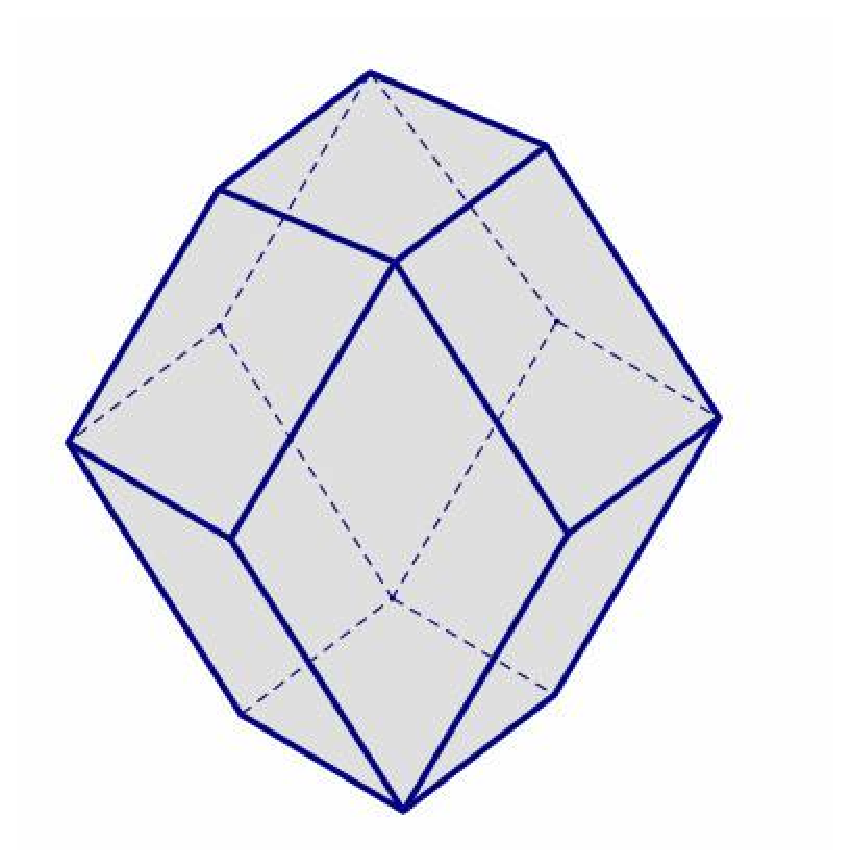
\includegraphics[width=5cm,height=4cm]{timg}

\end{Ex}

\begin{Ex}
  下图是否是哈密顿图?若是,找出一个哈密顿圈?若不是,说明理由。

  \centering
      \begin{tikzpicture}[auto,
    specification/.style ={circle, draw, thick, inner sep = 0pt, minimum size=2mm}]
   \node[specification] (A)  at (90:1.6cm)  {};
   \node[specification] (B)  at (210:1.6cm)  {};
   \node[specification] (C)  at (330:1.6cm)  {};
   \node[specification] (D)  at (90:0.8cm)  {};
   \node[specification] (E)  at (210:0.8cm)  {};
   \node[specification] (F)  at (330:0.8cm)  {};
   \node[specification] (G)  at (210:2.4cm)  {};
   \node[specification] (H)  at (330:2.4cm)  {};
   \node[specification] (I)  at (0,0)  {};
   
   
   \draw[thick] (A) to  (B);
   \draw[thick] (B) to  (C);
   \draw[thick] (C) to  (A);
   \draw[thick] (D) to  (E);
   \draw[thick] (E) to  (F);
   \draw[thick] (F) to  (D);
   \draw[thick] (D) to  (G);
   \draw[thick] (D) to  (H);
   \draw[thick] (H) to  (B);
   \draw[thick] (G) to  (C);
   \draw[thick] (A) to  (D);
   \draw[thick] (C) to  (F);
   \draw[thick] (B) to  (E);
   \draw[thick] (I) to  (D);
   \draw[thick] (I) to  (E);
   \draw[thick] (I) to  (F);
   \draw[thick] (G) to  (B);
   \draw[thick] (H) to  (C);
   \draw[thick] (B) to [bend right = 10] (I);
   \draw[thick] (C) to [bend left = 10] (I);
 \end{tikzpicture}


\end{Ex}


\begin{Ex}
  下图是否是哈密顿图?若是,找出一个哈密顿圈?若不是,说明理由。

\centering  
      \begin{tikzpicture}[auto,
    specification/.style ={circle, draw, thick, inner sep = 0pt, minimum size=2mm}]
   \node[specification] (A)  at (18:2.3cm)  {};
   \node[specification] (B)  at (90:2.3cm)  {};
   \node[specification] (C)  at (162:2.3cm)  {};
   \node[specification] (D) at (234:2.3cm)  {};
   \node[specification] (E)  at (306:2.3cm)  {};
   \node[specification] (F)  at (18:1.5cm)  {};
   \node[specification] (G)  at (90:1.5cm)  {};
   \node[specification] (H)  at (162:1.5cm)  {};
   \node[specification] (I) at (234:1.5cm)  {};
   \node[specification] (J)  at (306:1.5cm)  {};
   \node[specification] (K)  at (0,0)  {};
   
   
   
   \draw[thick] (A) to  (B);
   \draw[thick] (B) to  (C);
   \draw[thick] (C) to  (D);
   \draw[thick] (D) to  (E);
   \draw[thick] (E) to  (A);
   
   \draw[thick] (F) to  (G);
   \draw[thick] (G) to  (H);
   \draw[thick] (H) to  (I);
   \draw[thick] (I) to  (J);
   \draw[thick] (J) to  (F);
   
   \draw[thick] (B) to  (G);
   \draw[thick] (D) to  (I);
   \draw[thick] (E) to  (J);
   \draw[thick] (K) to  (H);
   \draw[thick] (K) to  (J);

 \end{tikzpicture}
\end{Ex}

\begin{Ex}
  下图是否是哈密顿图?若是,找出一个哈密顿圈?若不是,说明理由。

  \centering
      \begin{tikzpicture}[auto,
    specification/.style ={circle, draw, thick, inner sep = 0pt, minimum size=2mm}]
   \node[specification] (A)  at (18:2.3cm)  {};
   \node[specification] (B)  at (90:2.3cm)  {};
   \node[specification] (C)  at (162:2.3cm)  {};
   \node[specification] (D) at (234:2.3cm)  {};
   \node[specification] (E)  at (306:2.3cm)  {};
   \node[specification] (F)  at (18:1.5cm)  {};
   \node[specification] (G)  at (90:1.5cm)  {};
   \node[specification] (H)  at (162:1.5cm)  {};
   \node[specification] (I) at (234:1.5cm)  {};
   \node[specification] (J)  at (306:1.5cm)  {};
   
   
   \draw[thick] (A) to  (B);
   \draw[thick] (B) to  (C);
   \draw[thick] (C) to  (D);
   \draw[thick] (D) to  (E);
   \draw[thick] (E) to  (A);
   \draw[thick] (A) to  (F);
   \draw[thick] (B) to  (G);
   \draw[thick] (C) to  (H);
   \draw[thick] (D) to  (I);
   \draw[thick] (E) to  (J);
   \draw[thick] (G) to  (I);
   \draw[thick] (I) to  (F);
   \draw[thick] (F) to  (H);
   \draw[thick] (H) to  (J);
   \draw[thick] (J) to  (G);

 \end{tikzpicture}
\end{Ex}


\begin{Ex}
  以下4个图中,存在一个哈密顿圈的是$\underline{\quad\quad}$。
  \vspace{0.5cm}

  A.
    \begin{minipage}{0.18\linewidth}
    \centering
    \begin{tikzpicture}[auto,
    specification/.style ={circle, draw, thick}, scale = 0.8]
   \node[specification] (A)  at (0,0)  {};
   \node[specification] (B)  at (1,0)  {};
   \node[specification] (C)  at (2,0)  {};
   \node[specification] (D)  at (0,1)  {};
   \node[specification] (E)  at (1,1)  {};
   \node[specification] (F)  at (2,1)  {};
   \node[specification] (G)  at (0,2)  {};
   \node[specification] (H)  at (1,2)  {};
   \node[specification] (I)  at (2,2)  {};

   \draw[thick] (A) to  (B);
   \draw[thick] (B) to  (C);
   \draw[thick] (D) to  (E);
   \draw[thick] (E) to  (F);
   \draw[thick] (G) to (H);
   \draw[thick] (H) to (I);
   \draw[thick] (A) to (D);
   \draw[thick] (B) to (E);
   \draw[thick] (C) to (F);
   \draw[thick] (D) to (G);
   \draw[thick] (E) to (H);
   \draw[thick] (F) to (I);
 \end{tikzpicture}
\end{minipage}\hfill
  B.
    \begin{minipage}{0.18\linewidth}
    \centering
    \begin{tikzpicture}[auto,
    specification/.style ={circle, draw, thick}, scale = 0.8]
   \node[specification] (A)  at (0,0)  {};
   \node[specification] (B)  at (1,0)  {};
   \node[specification] (C)  at (2,0)  {};
   \node[specification] (D)  at (0,1)  {};
   \node[specification] (E)  at (1,1)  {};
   \node[specification] (F)  at (2,1)  {};
   \node[specification] (G)  at (0,2)  {};
   \node[specification] (H)  at (1,2)  {};
   \node[specification] (I)  at (2,2)  {};

   \draw[thick] (A) to  (B);
   \draw[thick] (B) to  (C);
   \draw[thick] (D) to  (E);
   \draw[thick] (E) to  (F);
   \draw[thick] (G) to (H);
   \draw[thick] (H) to (I);
   \draw[thick] (A) to (D);
   \draw[thick] (B) to (E);
   \draw[thick] (C) to (F);
   \draw[thick] (D) to (G);
   \draw[thick] (E) to (H);
   \draw[thick] (F) to (I);
   \draw[thick] (D) to (H);

 \end{tikzpicture}
\end{minipage}\hfill
      C.
    \begin{minipage}{0.18\linewidth}
    \centering
    \begin{tikzpicture}[auto,
    specification/.style ={circle, draw, thick}, scale=0.8]
   \node[specification] (A)  at (0,0)  {};
   \node[specification] (B)  at (1,0)  {};
   \node[specification] (C)  at (2,0)  {};
   \node[specification] (D)  at (0,1)  {};
   \node[specification] (E)  at (1,1)  {};
   \node[specification] (F)  at (2,1)  {};
   \node[specification] (G)  at (0,2)  {};
   \node[specification] (H)  at (1,2)  {};
   \node[specification] (I)  at (2,2)  {};

   \draw[thick] (A) to  (B);
   \draw[thick] (B) to  (C);
   \draw[thick] (D) to  (E);
   \draw[thick] (E) to  (F);
   \draw[thick] (G) to (H);
   \draw[thick] (H) to (I);
   \draw[thick] (A) to (D);
   \draw[thick] (B) to (E);
   \draw[thick] (C) to (F);
   \draw[thick] (D) to (G);
   \draw[thick] (E) to (H);
   \draw[thick] (F) to (I);
   \draw[thick] (D) to (H);
   \draw[thick] (B) to (F);
 \end{tikzpicture}
\end{minipage}\hfill
      D.
    \begin{minipage}{0.18\linewidth}
    \centering
    \begin{tikzpicture}[auto,
    specification/.style ={circle, draw, thick}, scale=0.8]
   \node[specification] (A)  at (0,0)  {};
   \node[specification] (B)  at (1,0)  {};
   \node[specification] (C)  at (2,0)  {};
   \node[specification] (D)  at (0,1)  {};
   \node[specification] (E)  at (1,1)  {};
   \node[specification] (F)  at (2,1)  {};
   \node[specification] (G)  at (0,2)  {};
   \node[specification] (H)  at (1,2)  {};
   \node[specification] (I)  at (2,2)  {};

   \draw[thick] (A) to  (B);
   \draw[thick] (B) to  (C);
   \draw[thick] (D) to  (E);
   \draw[thick] (E) to  (F);
   \draw[thick] (G) to (H);
   \draw[thick] (H) to (I);
   \draw[thick] (A) to (D);
   \draw[thick] (B) to (E);
   \draw[thick] (C) to (F);
   \draw[thick] (D) to (G);
   \draw[thick] (E) to (H);
   \draw[thick] (F) to (I);
   \draw[thick] (E) to (I);

 \end{tikzpicture}
\end{minipage}\hfill

\end{Ex}

\begin{Ex}
  以下4个图中,不存在哈密顿路的是$\underline{\quad\quad}$。
  \vspace{0.5cm}

  A.
    \begin{minipage}{0.18\linewidth}
    \centering
    \begin{tikzpicture}[auto,
    specification/.style ={circle, draw, thick}, scale = 0.8]
   \node[specification] (A)  at (0,0)  {};
   \node[specification] (B)  at (1,0)  {};
   \node[specification] (C)  at (2,0)  {};
   \node[specification] (D)  at (0,1)  {};
   \node[specification] (E)  at (1,1)  {};
   \node[specification] (F)  at (2,1)  {};
   \node[specification] (G)  at (0,2)  {};
   \node[specification] (H)  at (1,2)  {};
   \node[specification] (I)  at (2,2)  {};

   \draw[thick] (A) to  (B);
   \draw[thick] (B) to  (C);
   \draw[thick] (D) to  (E);
   \draw[thick] (E) to  (F);
   \draw[thick] (G) to (H);
   \draw[thick] (H) to (I);
   \draw[thick] (A) to (D);
   \draw[thick] (B) to (E);
   \draw[thick] (C) to (F);
   \draw[thick] (D) to (G);
   \draw[thick] (E) to (H);
   \draw[thick] (F) to (I);
 \end{tikzpicture}
\end{minipage}\hfill
  B.
    \begin{minipage}{0.18\linewidth}
    \centering
    \begin{tikzpicture}[auto,
    specification/.style ={circle, draw, thick}, scale = 0.8]
   \node[specification] (A)  at (0,0)  {};
   \node[specification] (B)  at (1,0)  {};
   \node[specification] (C)  at (2,0)  {};
   \node[specification] (D)  at (0,1)  {};
   \node[specification] (E)  at (1,1)  {};
   \node[specification] (F)  at (2,1)  {};
   \node[specification] (G)  at (0,2)  {};
   \node[specification] (H)  at (1,2)  {};
   \node[specification] (I)  at (2,2)  {};

   \draw[thick] (A) to  (B);
   \draw[thick] (B) to  (C);
   \draw[thick] (A) to (D);
   \draw[thick] (B) to (E);
   \draw[thick] (C) to (F);
   \draw[thick] (D) to (G);
   \draw[thick] (E) to (H);
   \draw[thick] (F) to (I);

 \end{tikzpicture}
\end{minipage}\hfill
      C.
    \begin{minipage}{0.18\linewidth}
    \centering
    \begin{tikzpicture}[auto,
    specification/.style ={circle, draw, thick}, scale=0.8]
   \node[specification] (A)  at (0,0)  {};
   \node[specification] (B)  at (1,0)  {};
   \node[specification] (C)  at (2,0)  {};
   \node[specification] (D)  at (0,1)  {};
   \node[specification] (E)  at (1,1)  {};
   \node[specification] (F)  at (2,1)  {};
   \node[specification] (G)  at (0,2)  {};
   \node[specification] (H)  at (1,2)  {};
   \node[specification] (I)  at (2,2)  {};

   \draw[thick] (A) to  (B);
   \draw[thick] (B) to  (C);
   \draw[thick] (A) to (D);
   \draw[thick] (B) to (E);
   \draw[thick] (C) to (F);
   \draw[thick] (D) to (G);
   \draw[thick] (E) to (H);
   \draw[thick] (F) to (I);
   \draw[thick] (G) to (H);
 \end{tikzpicture}
\end{minipage}\hfill
      D.
    \begin{minipage}{0.18\linewidth}
    \centering
    \begin{tikzpicture}[auto,
    specification/.style ={circle, draw, thick}, scale=0.8]
   \node[specification] (A)  at (0,0)  {};
   \node[specification] (B)  at (1,0)  {};
   \node[specification] (C)  at (2,0)  {};
   \node[specification] (D)  at (0,1)  {};
   \node[specification] (E)  at (1,1)  {};
   \node[specification] (F)  at (2,1)  {};
   \node[specification] (G)  at (0,2)  {};
   \node[specification] (H)  at (1,2)  {};
   \node[specification] (I)  at (2,2)  {};

      \draw[thick] (A) to  (B);
   \draw[thick] (B) to  (C);
   \draw[thick] (A) to (D);
   \draw[thick] (B) to (E);
   \draw[thick] (C) to (F);
   \draw[thick] (D) to (G);
   \draw[thick] (E) to (H);
   \draw[thick] (F) to (I);
   \draw[thick] (G) to (H);
   \draw[thick] (H) to (I);

 \end{tikzpicture}
\end{minipage}\hfill



\end{Ex}



  \chapter{树}

\begin{Def}
    连通且无圈的无向图称为无向树,简称{\bfseries树}。 一个没有圈的无向图
    称为无向森林,简称{\bfseries森林}。
  \end{Def}
  \begin{Thm}
  设$G=(V,E)$为一个$(p,q)$图,下列各命题等价:
  \begin{enumerate}
  \item $G$为树;
  \item $G$的任意两个不同的顶点间有唯一的一条路联结;
  \item $G$为连通的且去掉任意一条边则得到一个不连通的图;
  \item $G$为连通的且$q = p - 1$;
  \item $G$中无圈且$q = p - 1$;
  \item $G$中无圈且$G$中任意两个不邻接的顶点间加一条边则得到一个含有圈的图。
  \end{enumerate}
  \end{Thm}
  \begin{proof}[证明]

    $1\Rightarrow2$

    用反证法。假设图$G$中存在两个顶点$u$和$v$,在它们之间存在两条不同的路$P_1$和
    $P_2$。由于$P_1\neq P_2$,$P_1$上存在一条边$x=u_1v_1$不在$P_2$上。由$P_1$和
    $P_2$上所有的顶点和边构成的$G$的子图记为$P_1\cup P_2$, 则$(P_1\cup P_2)- x$
    是连通的。于是,$(P_1\cup P_2)-x$中存在一条$u_1-v_1$路$P$,$P+x$为$G$的一个
    圈,矛盾。

    $2\Rightarrow3$

显然,图G为连通的。设$uv$为图$G$的任意一条联结顶点$u$和$v$的边,则$uv$为联结顶点
$u$和$v$的唯一的一条路,从图$G$中去掉边$uv$之后,顶点$u$和顶点$v$之间没有路,于
是得到了一个不连通的图。

$3\Rightarrow 4$

用数学归纳法证明,施归纳于顶点数$p$。

当$p=1$时,结论显然成立。

假设当$p=k$时结论成立,往证当$p=k+1$时结论也成立。
由图$G$为连通的且去掉任意一条边则得到一个不连通的图知图$G$中一定存在一个度为1的
顶点$v$。在图$G$中去掉顶点$v$及其与之关联的边,得到图$G'$。则图$G'$为连通的且去
掉任意一条边会得到一个不连通的图,由归纳假设,图$G'$中有$k-1$条边,于是图$G$中有
$k$条边,$q=p-1$成立,定理得证。

$4\Rightarrow 5$

用反证法。假设图$G$中有圈,则去掉圈上的一条边,得到的图仍然为连通的。如果新得到
的图仍然有圈,在圈上再去掉一条边,又会得到一个新的连通的图。如此继续下去,最终会
得到一个连通的没有圈的图。由从$1$到$4$的证明知最后到的图中有$p-1$条边,这与去掉
边之前图$G$中的边数$q=p-1$矛盾。

$5\Rightarrow 6$

设图$G$有$k$个支,则图$G$中的每个支连通且没有圈。设第$i$个支中含有$p_i$个顶点,
$q_i$条边。由$1$到$4$的证明知在第$i$个支中$q_i=p_i-1$。将所有支的边数和顶点数相
加,可得$q = p-k$。于是$k=1$,从而$G$为连通的。设$u$与$v$为图$G$的任意两个不
邻接的顶点,则$u$与$v$之间存在一条路,再在$u$与$v$之间加一条边,则得到一个圈。

$6\Rightarrow 1$

设$u$和$v$为图$G$的任意两个顶点。如果$u$和$v$邻接,则$u$和$v$之间有一条路。如果
$u$和$v$之间不邻接,则在$u$和$v$之间加一条边,会得到一个圈。在该圈上将边$uv$去掉,
则得到$u$与$v$之间的一条路。这证明了$G$为连通的。
\end{proof}
  \begin{Def}
    设$G=(V,E)$为一个图,$G$的一个生成子图$T=(V,F)$如果是树,则称$T$为$G$的{\bfseries 生成树}。
  \end{Def}
  \begin{Thm}
    图$G$有生成树的充分必要条件是$G$为一个连通图。
  \end{Thm}
  \begin{Def}
    设$v$为图$G$的一个顶点,如果$G-v$的支数大于$G$的支数,则称顶点$v$为图$G$的一个{\bfseries 割点}。
  \end{Def}
  \centering
    \begin{tikzpicture}[auto,
    specification/.style ={circle, draw, thick}]
   \node[specification] (A) [label=90:$v_1$] at (1,1)  {};
   \node[specification] (B) [label=90:$v_2$] at (2,0)  {};
   \node[specification] (C) [label=-90:$v_3$] at (1,-1)  {};
   \node[specification] (D) [label=180:$v_4$] at (0,0)  {};
   \node[specification] (E) [label=90:$v_5$] at (4,0) {};
   \node[specification] (F) [label=90:$v_6$] at (5,1) {};
   \node[specification] (G) [label=-90:$v_7$] at (5,-1) {};
   \draw[thick] (A) to  (B);
   \draw[thick] (B) to  (C);
   \draw[thick] (C) to  (D);
   \draw[thick] (D) to  (A);
   \draw[thick] (A) to  (C);
   \draw[thick] (B) to  (D);   
   \draw[thick] (B) to  (E);
   \draw[thick] (E) to  (F);
   \draw[thick] (F) to  (G);
   \draw[thick] (G) to  (E);
 \end{tikzpicture}  
  \begin{Thm}
    设$v$为连通图$G=(V,E)$的一个割点,则下列命题等价:
    \begin{enumerate}
    \item $v$为图$G$的一个割点;
    \item 集合$V\setminus \{v\}$有一个二划分$\{U,W\}$, 使得对任意的$u \in U$,$w \in W$,$v$在联结$u$和$w$的每条路上;
    \item 存在与$v$不同的两个顶点$u$和$w$,使得$v$在每一条$u$与$w$间的路上。
    \end{enumerate}
  \end{Thm}
  \centering
    \begin{tikzpicture}[auto,
    specification/.style ={circle, draw, thick}]
   \node[specification] (A) [label=90:$v_1$] at (1,1)  {};
   \node[specification] (B) [label=90:$v_2$] at (2,0)  {};
   \node[specification] (C) [label=-90:$v_3$] at (1,-1)  {};
   \node[specification] (D) [label=180:$v_4$] at (0,0)  {};
   \node[specification] (E) [label=90:$v_5$] at (4,0) {};
   \node[specification] (F) [label=90:$v_6$] at (5,1) {};
   \node[specification] (G) [label=-90:$v_7$] at (5,-1) {};
   \draw[thick] (A) to  (B);
   \draw[thick] (B) to  (C);
   \draw[thick] (C) to  (D);
   \draw[thick] (D) to  (A);
   \draw[thick] (A) to  (C);
   \draw[thick] (B) to  (D);   
   \draw[thick] (B) to  (E);
   \draw[thick] (E) to  (F);
   \draw[thick] (F) to  (G);
   \draw[thick] (G) to  (E);
 \end{tikzpicture}  
  \begin{Def}
   图$G$的一条边$x$称为$G$的一座{\bfseries 桥},如果$G-x$的支数大于$G$的支数。
  \end{Def}
  \centering
    \begin{tikzpicture}[auto,
    specification/.style ={circle, draw, thick}]
   \node[specification] (A) [label=90:$v_1$] at (1,1)  {};
   \node[specification] (B) [label=90:$v_2$] at (2,0)  {};
   \node[specification] (C) [label=-90:$v_3$] at (1,-1)  {};
   \node[specification] (D) [label=180:$v_4$] at (0,0)  {};
   \node[specification] (E) [label=90:$v_5$] at (4,0) {};
   \node[specification] (F) [label=90:$v_6$] at (5,1) {};
   \node[specification] (G) [label=-90:$v_7$] at (5,-1) {};
   \draw[thick] (A) to  (B);
   \draw[thick] (B) to  (C);
   \draw[thick] (C) to  (D);
   \draw[thick] (D) to  (A);
   \draw[thick] (A) to  (C);
   \draw[thick] (B) to  (D);   
   \draw[thick] (B) to  (E);
   \draw[thick] (E) to  (F);
   \draw[thick] (F) to  (G);
   \draw[thick] (G) to  (E);
 \end{tikzpicture}  

   \begin{Thm}
    设$x$为连通图$G=(V,E)$的一条边,则下列命题等价:
    \begin{enumerate}
    \item $x$为$G$的桥;
    \item $x$不在$G$的任一圈上;
    \item 存在$V$的一个划分$\{U,W\}$,使得对任意的$u \in U, w \in W$,$x$在每一条联结$u$与$w$的路上;
    \item 存在$G$的不同顶点$u$和$v$,使得边$x$在联结$u$和$v$的每条路上。
    \end{enumerate}
  \end{Thm}
  \centering
    \begin{tikzpicture}[auto,
    specification/.style ={circle, draw, thick}]
   \node[specification] (A) [label=90:$v_1$] at (1,1)  {};
   \node[specification] (B) [label=90:$v_2$] at (2,0)  {};
   \node[specification] (C) [label=-90:$v_3$] at (1,-1)  {};
   \node[specification] (D) [label=180:$v_4$] at (0,0)  {};
   \node[specification] (E) [label=90:$v_5$] at (4,0) {};
   \node[specification] (F) [label=90:$v_6$] at (5,1) {};
   \node[specification] (G) [label=-90:$v_7$] at (5,-1) {};
   \draw[thick] (A) to  (B);
   \draw[thick] (B) to  (C);
   \draw[thick] (C) to  (D);
   \draw[thick] (D) to  (A);
   \draw[thick] (A) to  (C);
   \draw[thick] (B) to  (D);   
   \draw[thick] (B) to  (E);
   \draw[thick] (E) to  (F);
   \draw[thick] (F) to  (G);
   \draw[thick] (G) to  (E);
 \end{tikzpicture}  
  \begin{Def}
    设$G = (V,E)$为图,$S \subseteq E$。如果从$G$中去掉$S$中的所有边得到的图$G-S$的支数大于$G$的支数,而去掉$S$的任一真子集中的边得到的图的支数不大于$G$的支数,则称$S$为$G$的一个{\bfseries 割集}。
  \end{Def}
  \centering
    \begin{tikzpicture}[auto,
    specification/.style ={circle, draw, thick}]
   \node[specification] (A) [label=90:$v_1$] at (1,1)  {};
   \node[specification] (B) [label=90:$v_2$] at (2,0)  {};
   \node[specification] (C) [label=-90:$v_3$] at (1,-1)  {};
   \node[specification] (D) [label=180:$v_4$] at (0,0)  {};
   \node[specification] (E) [label=90:$v_5$] at (4,0) {};
   \node[specification] (F) [label=90:$v_6$] at (5,1) {};
   \node[specification] (G) [label=-90:$v_7$] at (5,-1) {};
   \draw[thick] (A) to  (B);
   \draw[thick] (B) to  (C);
   \draw[thick] (C) to  (D);
   \draw[thick] (D) to  (A);
   \draw[thick] (A) to  (C);
   \draw[thick] (B) to  (D);   
   \draw[thick] (B) to  (E);
   \draw[thick] (E) to  (F);
   \draw[thick] (F) to  (G);
   \draw[thick] (G) to  (E);
 \end{tikzpicture}  

\chapter{}
%%% Local Variables:
%%% mode: latex
%%% TeX-master: "book_chapter7"
%%% End:

  \chapter{连通度}
  \begin{Def}
    图$G$的{\bfseries 顶点连通度}是指为了产生一个不连通图或平凡图所需要从$G$中去掉的最少顶点数目, 记为$\kappa (G)$。
  \end{Def}
  \begin{Def}
    图$G$的{\bfseries 边连通度}是指为了产生一个不连通图或平凡图所需要从$G$中去掉的最少边的数目, 记为$\lambda (G)$。
  \end{Def}
  \begin{Def}
    设$G$是一个图,如果$\kappa (G) \geq n$,则称$G$是{\bfseries $n$-顶点连通}的,简称$n$-连
    通;如果$\lambda (G) \geq n$,则称$G$是{\bfseries $n$-边连通}的。
  \end{Def}

\begin{Ex}
  构造一个图$G$,使得$\kappa(G)=3,\lambda(G)=4,\delta(G)=5$。
\end{Ex}

  \input{matching}
  \chapter{平面图和图的着色}
  \begin{Def}
    图$G$称为被嵌入平(曲)面$S$内,如果$G$的图解已画在$S$上,而且任意两条边均不相交(除可能在端点相交外)。
已嵌入平面内的图称为{\bfseries 平面图}。如果一个图可以嵌入平面,则称此图为{\bfseries 可平面的}。
\end{Def}
  \begin{Def}
    平面图$G$把平面分成了若干个区域,这些区域都是连通的,称之为$G$的面,其中无界的那个连通区域称为$G$的外部面,其余的连通区域称为$G$的内部面。
  \end{Def}
  \begin{center}
  \includegraphics[width=4cm,height=3cm]{face}
\end{center}
\begin{Thm}[欧拉公式]
    如果有$p$个顶点$q$条边的平面连通图$G$有$f$个面,则
      $p - q + f = 2$
    \end{Thm}
    \begin{proof}[证明]
\mbox{}\par{}
    用数学归纳法证明,施归纳于面数$f$。

  (1)当$f=1$时,$G$中无圈,又因为$G$是连通的,所以$G$是树。从而
  $q=p-1$,$p-q+f=2$成立。

  (2)假设当$f=k$时结论成立,往证当$f=k+1$时结论也成立。假设$G$有$k+1$个面,
  $k\geq 1$。此时$G$至少有一个内部面,从而有一个圈。从这个圈上去掉一条边$x$,则
  $G-x$就是一个有$p$个顶点,$q-1$条边,$k$个面的平面连通图。由归纳假设,对
  $G-x$结论成立,即\[p-(q-1) + k =2\]
  因此,\[p-q+ (k+1) =2\]
  即当$f=k+1$时结论也成立。
\end{proof}
 \begin{Cor}
    若平面图$G$有$p$个顶点$q$条边且每个面都是由长为$n$的圈围成的,则
    \begin{equation*}
      q = n(p-2)/(n-2)
    \end{equation*}
  \end{Cor}
一个{\bfseries 最大可平面图}是一个可平面图,对此可平面图中不能再加入边而不破坏其可平面性。
  \begin{Cor}
    设$G$为一个有$p$个顶点$q$条边的最大可平面图,$p \geq 3$,则$G$的每个面都为三角形,而且$q=3p-6$。
  \end{Cor}
  \begin{Cor}
    设$G$为一个$(p,q)$可平面连通图,而且$G$的每个面都是由一个长为$4$的圈围成的,则$q=2p-4$。
  \end{Cor}
  \begin{Cor}
    若$G$为一个有$p$个顶点$q$条边的可平面图,$p\geq 3$,则$q \leq 3p - 6$;进一步,若$G$中没有三角形,则$q \leq 2p -4$。
  \end{Cor}
     \centering
    \begin{tikzpicture}[auto,
    specification/.style ={circle, draw, thick, inner sep = 0pt, minimum size=2mm}]
   \node[specification] (A)  at (0:2cm)  {};
   \node[specification] (B)  at (60:2cm)  {};
   \node[specification] (C)  at (120:2cm)  {};
   \node[specification] (D) at (180:2cm)  {};
   \node[specification] (E)  at (240:2cm)  {};   
   \node[specification] (F)  at (300:2cm)  {};   
   \node[specification] (G)  at (300:0.5cm)  {};
   \node[specification] (H)  at (180:3cm)  {};
   
   
   \draw[thick] (A) to  (B);
   \draw[thick] (B) to  (C);
   \draw[thick] (C) to  (D);
   \draw[thick] (D) to  (E);
   \draw[thick] (E) to  (F);
   \draw[thick] (F) to  (A);
   \draw[thick] (B) to  (E);
   \draw[thick] (F) to  (G);
   \draw[thick] (D) to  (H);   
 \end{tikzpicture}
 \begin{proof}[证明]
  不妨设$G$为连通的可平面图,否则可以加边使之变成连通的。由于每个面至少含有3条边,因此
  \[2q \geq 3f\]
  即
  \[\frac{2q}{3} \geq f\]
  因此,根据欧拉公式
  \[p - q + f = 2\]
  得
  \[p - q + \frac{2q}{3} \geq 2\]
  化简得:
  \[q \leq 3p - 6\]

  进一步,若$G$中没有三角形,则$G$中的每个面至少含有4条边,因此
  \[2q \geq 4f\]
  即
  \[\frac{q}{2} \geq f\]
  因此,根据欧拉公式
  \[p-q+f=2\]
  得
  \[p-q+ \frac{q}{2} \geq 2\]
  化简得:
  \[q \leq 2p - 4\]
\end{proof}

  \begin{Cor}
    $K_5$和$K_{3,3}$都不是可平面图。
  \end{Cor}
\vspace{1cm}
  \begin{minipage}{0.45\linewidth}
      \centering
    \begin{tikzpicture}[auto,
    specification/.style ={circle, draw, thick}]
   \node[specification] (A)   at (18:1.3cm)  {};
   \node[specification] (B)   at (90:1.3cm)  {};
   \node[specification] (C)   at (162:1.3cm)  {};
   \node[specification] (D)  at (234:1.3cm)  {};
   \node[specification] (E)   at (306:1.3cm)  {};      
   
   
   \draw[thick] (A) to  (B);
   \draw[thick] (B) to  (C);
   \draw[thick] (C) to  (D);
   \draw[thick] (D) to  (E);
   \draw[thick] (E) to  (A);
   \draw[thick] (A) to  (C);
   \draw[thick] (B) to  (E);
   \draw[thick] (C) to  (E);
   \draw[thick] (D) to  (A);
   \draw[thick] (B) to  (D);
 \end{tikzpicture}
    
  \end{minipage}
  \begin{minipage}{0.45\linewidth}
    \centering
    \begin{tikzpicture}[auto,
    specification/.style ={circle, draw, thick}]
   \node[specification] (A) at (0,0)  {};
   \node[specification] (B) at (1,0)  {};
   \node[specification] (C) at (2,0)  {};
   \node[specification] (D) at (0,1)  {};
   \node[specification] (E) at (1,1)  {};
   \node[specification] (F) at (2,1)  {};
   \draw[thick] (A) to  (D);
   \draw[thick] (A) to  (E);
   \draw[thick] (A) to (F);
   \draw[thick] (B) to (D);
   \draw[thick] (B) to (E);
   \draw[thick] (B) to (F);
   \draw[thick] (C) to (D);
   \draw[thick] (C) to (E);
   \draw[thick] (C) to (F);
 \end{tikzpicture}
  \end{minipage}
  \begin{proof}[证明]
  先证明$K_5$不是可平面图。用反证法,假设$K_5$为可平面图,其顶点数$p = 5$, 边数$q = 10$,此时
  \[q \leq 3p - 6\]
  即
  \[10 \leq 3 \times 5 - 6 = 9\]
  矛盾。因此$K_5$不是可平面图。

  接下来证明$K_{3,3}$不是可平面图。用反证法,假设$K_{3,3}$为可平面图,其顶点数为$p=6$,边数$q=9$,由$K_{3,3}$中没有三角形知
  \[q \leq 2p -4\]
  即
  \[9 \leq 2 * 6 - 4 = 8\]
  矛盾。因此$K_{3,3}$不是可平面图。
\end{proof}
  \begin{Cor}
    每个可平面图$G$中顶点度的最小值不超过5,即$\delta (G) \leq 5$。
  \end{Cor}
  \begin{proof}[证明(证法一)]
  当图$G$的顶点数$p=1,2$时,结论显然成立。当$p\geq 3$时,
  设可平面图$G$有$q$条边,则
  \[\delta p \leq 2q\]
  由$G$为可平面图知
  \[q \leq 3p - 6\]
  从而
  \[\delta p \leq 6p - 12\]
  两边同时除以$p$,得:
  \[\delta \leq 6 - \frac{12}{p}\]
  即
  \[\delta \leq 5\]
\end{proof}
\begin{proof}[证明(证法二)]
  当图$G$的顶点数$p=1,2$时,结论显然成立。
  当$p \geq 3$时,用反证法证明结论也成立。假设$\delta (G) \geq 6$,设$G$有$q$条边,则
  \[6p \leq 2q\]
  由$G$为可平面图知
  \[q \leq 3p - 6\]
  从而
  \[6p \leq 6p - 12\]
矛盾。  
\end{proof}

  \begin{Thm}
    设$G=(V,E)$为一个$(p,q)$平面哈密顿图,$C$为$G$的哈密顿圈。
    令$f_i$为$C$的内部由$i$条边围成的面的个数,$g_i$为$C$的外部$i$条边围成的面的个数,则
    \begin{align}
      &1 \cdot f_3 + 2 \cdot f_4 + 3 \cdot f_5 + \cdots = \sum_{i=3}^p(i-2)f_i = p - 2;\\
      &1 \cdot g_3 + 2 \cdot g_4 + 3 \cdot g_5 + \cdots = \sum_{i=3}^p(i-2)g_i = p - 2;\\
      &1 \cdot (f_3 - g_3) + 2 \cdot (f_4 - g_4) + 3 \cdot (f_5 - g_5) + \cdots = \sum_{i=3}^p(i-2)(f_i - g_i) = 0
    \end{align}
  \end{Thm}
    \centering
  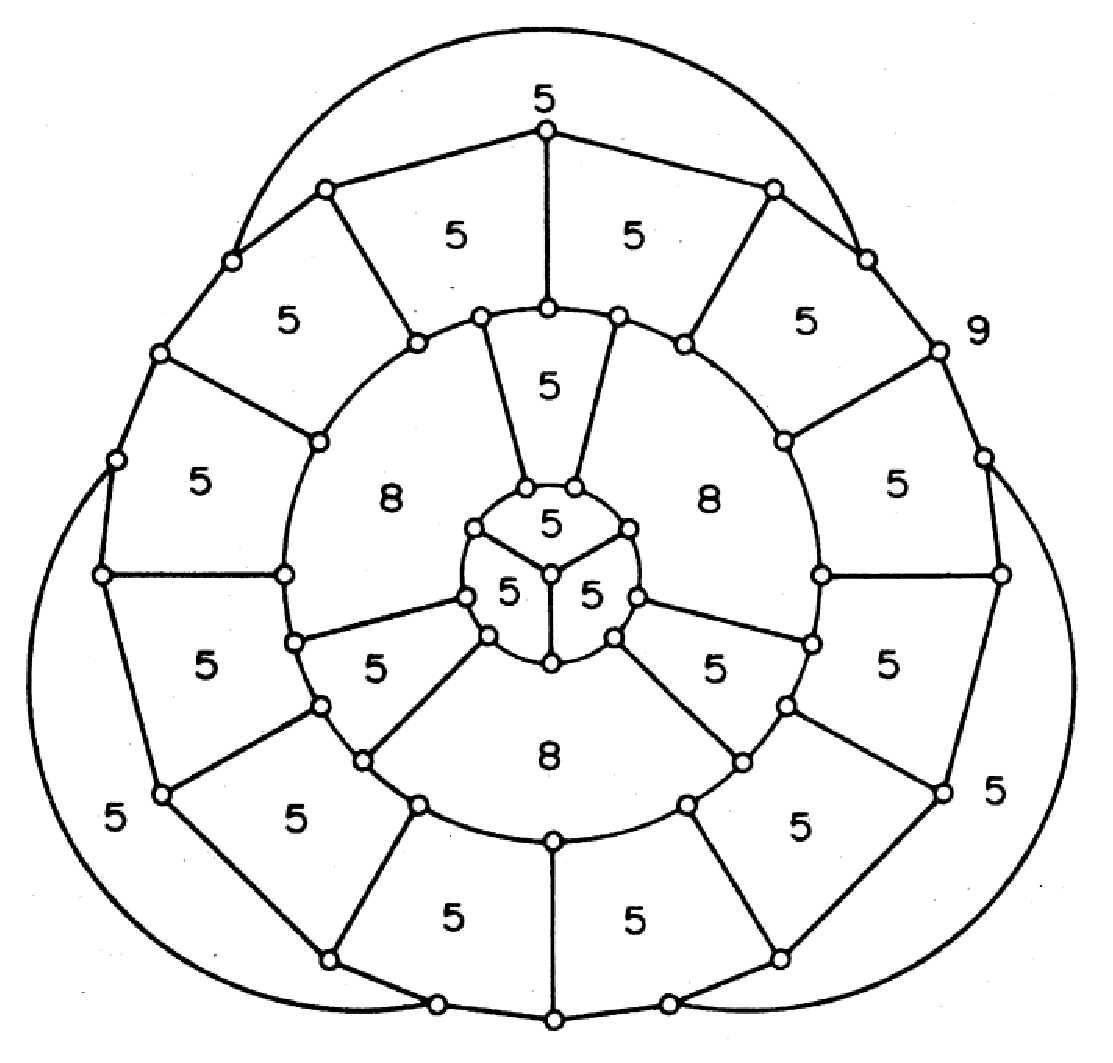
\includegraphics[width=7cm, height=6cm]{grinberg}
  \begin{Def}
    设$x=uv$为图$G=(V,E)$的一条边,又$w$不是$G$的顶点,则当用边$uw$和$wv$代替边$x$时,就称$x$被细分。如果$G$的某些条边被细分,产生的图称为$G$的细分图。
  \end{Def}
  \begin{Def}
    两个图称为同胚的,如果它们都可以从同一个图通过一系列的边细分得到。
  \end{Def}
  \begin{Thm}
    一个图为可平面的充分必要条件是它没有同胚于$K_5$或$K_{3,3}$的子图。
  \end{Thm}
  \begin{Def}
    一个图$G$的一个初等收缩由等同两个临接的顶点$u$和$v$得到,即从$G$中去掉$u$和$v$,然后再加上一个新顶点$w$,使得$w$临接于所有临接于$u$或$v$的顶点。一个图$G$可以收缩到图$H$,如果$H$可以从$G$经过一系列的初等收缩得到。
  \end{Def}
  \begin{Thm}
    一个图为可平面的当且仅当它没有一个可以收缩到$K_5$或$K_{3,3}$的子图。
  \end{Thm}
  \begin{Def}
    设$G=(V,E)$为一个平面图,由$G$按照如下方法构造一个图$G^*$,$G^*$称为$G$的对偶图:对$G$的每个面$f$对应地有$G^*$的一个顶点$f^*$;对$G$的每条边$e$对应地有$G^*$的一条边$e^*$:$G^*$的两个顶点$f^*$与$g^*$由边$e^*$联结,当且仅当$G$中与顶点$f^*$与$g^*$对应的面$f$与$g$有公共边$e$,如果某条边$x$仅在一个面中出现而不是两个面的公共边,则在$G^*$中这个面对应的顶点有一个环。
  \end{Def}
  \begin{Def}
    图的一种{\bfseries 着色}是指对图的每个顶点指定一种颜色,使得没有两个临接的顶点有同一种颜色。图$G$的一个{\bfseries $n-$着色}是用$n$种颜色对$G$的着色。
  \end{Def}
  \begin{Def}
    图$G$的{\bfseries 色数}是使$G$为$n-$着色的数$n$的最小值,图$G$的色数记为$\chi(G)$。若$\chi (G) \leq n$,则称$G$为{\bfseries $n-$可着色}的。若$\chi (G) = n$,则称$G$为{\bfseries $n$色}的。
  \end{Def}
  \begin{Thm}
    一个图是可双色的当且仅当它没有奇数长的圈。
  \end{Thm}
  \renewcommand{\figurename}{图}
\begin{figure}\centering
  \includegraphics[width=4cm,height=3cm]{color26}
      \caption{用两种颜色对一个没有奇数长的圈的图进行着色的示意图}
    \label{fig:twocoloring}  
    \end{figure}
    \begin{proof}[证明]
    设图$G$为可双色的,则显然图$G$没有奇数长的圈。这是因为假设图$G$有奇数长的圈$C$,
    则$C$是3色的,从而$\chi(G) \geq 3$,与$G$是可双色的矛盾。

      设图$G$没有奇数长的圈,以下给出一种用两种颜色对$G$的顶点进行着色的算法,从而证明图$G$是可双色的。不妨设图$G$是连通的,否则可以对图$G$的每个连通分量分别进行着色。任取$G$的一个顶点$a$,对其着红色,然后对与顶点$a$邻接的顶点着蓝色,接下来对所有与已经着色的顶点相邻接的顶点着红色,这样依次下去,每次都对所有与已经着色的顶点相邻接的顶点着与前一次的着色不同的另一种颜色。如图~\ref{fig:twocoloring}所示该算法结束时用至多两种颜色对$G$的顶点进行了着色。

以下证明每次对所有与已经着色的顶点相邻接的顶点着与前一次的着色不同的另一种颜色时,
不会产生相邻的两个顶点着以相同颜色的情况,从而保证前面的算法是正确的。用反证法。
假设对顶点$u$进行着色时,不妨设对其着红色,已经有一个与之相邻的顶点$v$着了红色。
从着色的过程知,从顶点$a$到顶点$u$之间有一条路$P_1$,其上的顶点依次着了红色和蓝色,
从顶点$a$到顶点$v$之间也有一条路$P_2$,其上的顶点依次着了红色和蓝色。
取$P_1$和$P_2$的最后一个公共的顶点$x$,则$P_1$上从顶点$u$到顶点$x$的路与$P_2$上从顶点$x$到顶点$v$的路和边$vu$一起构成一个圈,该圈上$u$和$v$着相同的颜色,其他各顶点依次着不同的颜色,因此其长度为奇数,与$G$中没有奇数长的圈矛盾。 
  \end{proof}

  \begin{Thm}
    设$\Delta = \Delta (G)$为图$G$的顶点度的最大值,则$G$为$(\Delta+1)-$可着色的。
  \end{Thm}
  \begin{proof}[证明]用数学归纳法证明,施归纳于顶点数$p$。

    (1)当$p=1$时,结论显然成立。

    (2)假设当$p=k(k\geq 1)$时结论成立,往证当$p=k+1$时结论也成立。设$v$为$G$中的任意一个顶点,由归纳假设,$G-v$是$\Delta(G-v)+1$可着色的。又由于$\Delta(G-v) \leq \Delta$,从而$G-v$为$\Delta+1$可着色的。假设已经用至多$\Delta+1$种颜色对$G-v$进行了顶点着色,使得任意相邻的顶点着不同的颜色,那么此时在$G$中与$v$邻接的顶点用了至多$\Delta$种颜色,用另外一种不同的颜色对顶点$v$进行着色,从而用至多$\Delta+1$种颜色就可以对$G$的顶点进行着色使得相邻的顶点着不同的颜色,即$G$为$\Delta + 1$可着色的。
    
  \end{proof}
  \begin{Thm}
    如果$G$是一个连通图且不是完全图也不是奇数长的圈,则$G$为$\Delta(G)-$可着色的。
  \end{Thm}
  \begin{Thm}
    每个平面图为$6-$可着色的。
  \end{Thm}
  \begin{Thm}
    每个平面图为$5-$可着色的。
  \end{Thm}
  \begin{proof}[证明]
  用数学归纳法证明,施归纳于图的顶点数$p$。

  (1)当$p=1$时,结论显然成立。

  (2)假设当$p<k$时结论成立,往证当$p=k$时结论也成立。设平面图$G$有$k$个顶点,则图$G$中一定有一个顶点$v$使得$\deg v \leq 5$。于是,$G-v$是一个有$k-1$个顶点的平面图,由归纳假设,$G-v$是$5-$可着色的。假设用至多5种颜色对$G-v$进行了着色。

  如果$\deg v \leq 4$,则在$G-v$中用至多5种颜色进行顶点着色时,在$G$中与$v$邻接的顶点至多用了$4$种颜色,如图~\ref{fig:coloring}所示。此时,用另外一种不同的颜色对顶点$v$进行着色,这样用至多5种颜色就可以对$G$的顶点进行着色,从而图$G$是$5-$可着色的。
\begin{figure}
  \begin{minipage}{0.49\linewidth}
    \centering
   \begin{tikzpicture}[auto,
    specification/.style ={circle, draw, thick, inner sep = 0pt, minimum size=2mm}]
   \node[specification, fill = blue] (A)  [label=0:$v_1$] at (18:1.3cm)  {};
   \node[specification, fill = red] (C)  [label=180:$v_4$] at (162:1.3cm)  {};
   \node[specification, fill = green] (D) [label=180:$v_3$] at (234:1.3cm)  {};
   \node[specification, fill = orange] (E)  [label=0:$v_2$] at (306:1.3cm)  {};      
   \node[specification] (o)  [label=0:$v$] at (0,0)  {};      
   \draw[thick] (A) to  (o);
   \draw[thick] (C) to  (o);
   \draw[thick] (D) to  (o);
   \draw[thick] (E) to  (o);
 \end{tikzpicture}
    \caption{$\deg v \leq 4$的情况}
    \label{fig:coloring}  
  \end{minipage}
  \begin{minipage}{0.49\linewidth}
    \centering
   \begin{tikzpicture}[auto,
    specification/.style ={circle, draw, thick, inner sep = 0pt, minimum size=2mm}]
   \node[specification, fill = blue] (A)  [label=0:$v_2$] at (18:1.3cm)  {};
   \node[specification, fill = purple] (B)  [label=90:$v_1$] at (90:1.3cm)  {};
   \node[specification, fill = red] (C)  [label=180:$v_5$] at (162:1.3cm)  {};
   \node[specification, fill = green] (D) [label=180:$v_4$] at (234:1.3cm)  {};
   \node[specification, fill = orange] (E)  [label=0:$v_3$] at (306:1.3cm)  {};      
   \node[specification] (o)  [label=0:$v$] at (0,0)  {};      
   
   
   \draw[thick] (A) to  (o);
   \draw[thick] (B) to  (o);
   \draw[thick] (C) to  (o);
   \draw[thick] (D) to  (o);
   \draw[thick] (E) to  (o);
 \end{tikzpicture}
  \caption{$\deg v = 5$的情况}
  \label{fig:collision}
  \end{minipage}
\end{figure}    


如果$\deg v = 5$,与$v$邻接的$5$个顶点$v_1,v_2,v_3,v_4,v_5$在$G-v$中用$c_1,c_2,c_3,c_4,c_5$ 5种颜色进行了着色。如果$c_1,c_2,c_3,c_4,c_5$中有两种颜色是相同的,则$c_1$, $c_2$, $c_3$, $c_4$, $c_5$中至多有$4$种颜色,用另外一种颜色对顶点$v$进行着色,这样用至多5种颜色就可以对$G$的顶点进行着色。以下考虑$c_1,c_2,c_3,c_4,c_5$中的各种颜色互不相同的情况,如图~\ref{fig:collision}所示。在图$G$中,与顶点$v$邻接的$5$个顶点$v_1,v_2,v_3,v_4,v_5$中一定有两个顶点是不邻接的,否则图$G$中将有一个子图$K_5$,这与图$G$为平面图相矛盾。取其中不邻接的两个顶点$v_i$和$v_j$,在$G-v$中,将顶点$v_i$和顶点$v_j$视为同一个顶点$w$,即去掉顶点$v_i$和$v_j$,添加一个新的顶点$w$,原来与顶点$v_i$和顶点$v_j$相关联的边变为与顶点$w$相关联的边,得到的新的图记为$G'$,则$G'$仍然为平面图。由归纳假设,$G'$为$5-$可着色的。 设用至多$5$种颜色对$G'$进行了顶点着色。在$G-v$中,顶点$v_i$和顶点$v_j$都着与$w$相同的颜色,其他的顶点均与$G'$中相对应的顶点着相同的颜色,这样$G-v$用至多5种颜色就可以进行顶点着色。在这里,在$G$中与顶点$v$邻接的五个顶点$v_1,v_2,v_3,v_4,v_5$中用了4种颜色,用另外一种颜色对顶点$v$着色,这样用至多5种颜色就可以对$G$的顶点进行着色,从而图$G$为$5-$可着色的。
\end{proof}

  \begin{Thm}
    每个平面图为$4-$可着色的。
  \end{Thm}

\chapter{}
%%% Local Variables:
%%% mode: latex
%%% TeX-master: "book_chapter9"
%%% End:

  \input{coloring}
  \chapter{有向图}
  \begin{Def}
    设$V$为一个有穷非空集合,$A \subseteq V\times V \setminus \{(v,v)|v \in V\}$,二元组$D=(V,A)$称为一个{\bfseries 有向图}。$V$称为有向图$D$的{\bfseries 顶点集},$V$中的元素称为$D$的{\bfseries 顶点}。
    $A$称为$D$的{\bfseries 弧集}或{\bfseries 有向边集},$A$中的元素称为$D$的{\bfseries 弧}或{\bfseries 有向边}。如果$x = (u,v) \in A$,则$u$称为弧$x$的{\bfseries 起点},$v$称为弧$x$的{\bfseries 终点}。
  \end{Def}
    \centering
  \begin{tikzpicture}[auto,
    specification/.style ={circle, draw, thick}]
   \node[specification] (A) [label=-135:$v_1$] at (0,0)  {};
   \node[specification] (B) [label=135:$v_2$] at (0,2)  {};
   \node[specification] (C) [label=45:$v_3$] at (2,2)  {};
   \node[specification] (D) [label=-45:$v_4$] at (2,0)  {};
   \draw[thick, ->] (A) to  (B);
   \draw[thick, ->] (C) to  (B);
   \draw[thick, ->] (C) to  (D);
   \draw[thick, ->] (D) to  (A);
   \draw[thick, ->] (A) to  (C);
\end{tikzpicture}

  \begin{Def}
    如果$(u,v)$和$(v,u)$都是有向图$D$的弧,则称$(u,v)$与$(v,u)$为$D$的{\bfseries 对
      称弧}。如果$D$中不含对称弧,则称$D$为{\bfseries 定向图}。
  \end{Def}
  \begin{tikzpicture}[auto,
    specification/.style ={circle, draw, thick}]
   \node[specification] (A) [label=-135:$v_1$] at (0,0)  {};
   \node[specification] (B) [label=135:$v_2$] at (0,2)  {};
   \node[specification] (C) [label=45:$v_3$] at (2,2)  {};
   \node[specification] (D) [label=-45:$v_4$] at (2,0)  {};
   \draw[thick, ->] (A) to  (B);
   \draw[thick, ->] (C) to  (B);
   \draw[thick, ->] (C) to  (D);
   \draw[thick, ->] (D) to  (A);
   \draw[thick, ->] (A) to [bend left = 10] (C);
   \draw[thick, ->] (C) to [bend left = 10] (A);
\end{tikzpicture}\hspace{1cm}
  \begin{tikzpicture}[auto,
    specification/.style ={circle, draw, thick}]
   \node[specification] (A) [label=-135:$v_1$] at (0,0)  {};
   \node[specification] (B) [label=135:$v_2$] at (0,2)  {};
   \node[specification] (C) [label=45:$v_3$] at (2,2)  {};
   \node[specification] (D) [label=-45:$v_4$] at (2,0)  {};
   \draw[thick, ->] (A) to  (B);
   \draw[thick, ->] (C) to  (B);
   \draw[thick, ->] (C) to  (D);
   \draw[thick, ->] (D) to  (A);
   \draw[thick, ->] (A) to  (C);
\end{tikzpicture}

  \begin{Def}
    设$D=(V,A)$为一个有向图,$D$的{\bfseries 反向图}为有向图$D^T=(V,A^T)$,其中
    \[A^T=\{(u,v)|(v,u)\in A\}\]
  \end{Def}
\begin{tikzpicture}[auto,
    specification/.style ={circle, draw, thick}]
   \node[specification] (A) [label=-135:$v_1$] at (0,0)  {};
   \node[specification] (B) [label=135:$v_2$] at (0,2)  {};
   \node[specification] (C) [label=45:$v_3$] at (2,2)  {};
   \node[specification] (D) [label=-45:$v_4$] at (2,0)  {};
   \draw[thick, ->] (A) to  (B);
   \draw[thick, ->] (C) to  (B);
   \draw[thick, ->] (C) to  (D);
   \draw[thick, ->] (D) to  (A);
   \draw[thick, ->] (A) to  (C);
\end{tikzpicture}\hspace{1cm}
\begin{tikzpicture}[auto,
    specification/.style ={circle, draw, thick}]
   \node[specification] (A) [label=-135:$v_1$] at (0,0)  {};
   \node[specification] (B) [label=135:$v_2$] at (0,2)  {};
   \node[specification] (C) [label=45:$v_3$] at (2,2)  {};
   \node[specification] (D) [label=-45:$v_4$] at (2,0)  {};
   \draw[thick, ->] (B) to  (A);
   \draw[thick, ->] (B) to  (C);
   \draw[thick, ->] (D) to  (C);
   \draw[thick, ->] (A) to  (D);
   \draw[thick, ->] (C) to  (A);
\end{tikzpicture}

  \begin{Def}
    设$D=(V,A)$为一个有向图,$v$为$D$的任一顶点,以$v$为终点的弧称为$v$的{\bfseries 入弧};以$v$为始点的弧称为$v$的{\bfseries 出弧}。顶点$v$的入弧的条数称为$v$的{\bfseries 入度},记为$id(v)$;顶点$v$的出弧的条数称为$v$的{\bfseries 出度},记为$od(v)$。
  \end{Def}
\centering
\begin{tikzpicture}[auto,
    specification/.style ={circle, draw, thick}]
   \node[specification] (A) [label=-135:$v_1$] at (0,0)  {};
   \node[specification] (B) [label=135:$v_2$] at (0,2)  {};
   \node[specification] (C) [label=45:$v_3$] at (2,2)  {};
   \node[specification] (D) [label=-45:$v_4$] at (2,0)  {};
   \draw[thick, ->] (A) to  (B);
   \draw[thick, ->] (C) to  (B);
   \draw[thick, ->] (C) to  (D);
   \draw[thick, ->] (D) to  (A);
   \draw[thick, ->] (A) to  (C);
 \end{tikzpicture}
     \begin{Thm}
      设$D=(V,A)$为一个有向图,$|A| = q$,则
      \[\sum_{v\in V}id(v) = \sum_{v\in V}od(v) = q\]
      从而
      \[\sum_{v\in V}(id(v) + od(v)) = 2q\]
  \end{Thm}
\centering
\begin{tikzpicture}[auto,
    specification/.style ={circle, draw, thick}]
   \node[specification] (A) [label=-135:$v_1$] at (0,0)  {};
   \node[specification] (B) [label=135:$v_2$] at (0,2)  {};
   \node[specification] (C) [label=45:$v_3$] at (2,2)  {};
   \node[specification] (D) [label=-45:$v_4$] at (2,0)  {};
   \draw[thick, ->] (A) to  (B);
   \draw[thick, ->] (C) to  (B);
   \draw[thick, ->] (C) to  (D);
   \draw[thick, ->] (D) to  (A);
   \draw[thick, ->] (A) to  (C);
\end{tikzpicture}  

  \begin{Def}
     有向图$D=(V,A)$称为{\bfseries 完全有向图},如果\[A=V\times V \setminus \{(v,v)| v \in V\}\]
   \end{Def}
   \centering
  \begin{tikzpicture}[auto,
    specification/.style ={circle, draw, thick}]
   \node[specification] (A) [label=-135:$v_1$] at (0,0)  {};
   \node[specification] (B) [label=135:$v_2$] at (0,2)  {};
   \node[specification] (C) [label=45:$v_3$] at (2,2)  {};
   \node[specification] (D) [label=-45:$v_4$] at (2,0)  {};
   \draw[thick, ->] (A) to [bend left = 10]  (B);
   \draw[thick, ->] (B) to [bend left = 10]  (A);
   \draw[thick, ->] (B) to [bend left = 10]  (C);
   \draw[thick, ->] (C) to [bend left = 10]  (B);
   \draw[thick, ->] (C) to [bend left = 10]  (D);
   \draw[thick, ->] (D) to [bend left = 10]  (C);
   \draw[thick, ->] (D) to [bend left = 10]  (A);
   \draw[thick, ->] (A) to [bend left = 10]  (D);
   \draw[thick, ->] (B) to [bend left = 10]  (D);
   \draw[thick, ->] (D) to [bend left = 10]  (B);
   \draw[thick, ->] (A) to [bend left = 10]  (C);
   \draw[thick, ->] (C) to [bend left = 10]  (A);
\end{tikzpicture}   

  \begin{Def}
    有向图$D=(V,A)$的{\bfseries 补图}定义为$D^c=(V,A^c)$,其中
    \[A^c=(V \times V \setminus \{(v,v)|v \in V\})\setminus A\]
  \end{Def}
  \begin{tikzpicture}[auto,
    specification/.style ={circle, draw, thick}]
   \node[specification] (A) [label=-135:$v_1$] at (0,0)  {};
   \node[specification] (B) [label=135:$v_2$] at (0,2)  {};
   \node[specification] (C) [label=45:$v_3$] at (2,2)  {};
   \node[specification] (D) [label=-45:$v_4$] at (2,0)  {};
   \draw[thick, ->] (A) to  (B);
   \draw[thick, ->] (C) to  (B);
   \draw[thick, ->] (C) to  (D);
   \draw[thick, ->] (D) to  (A);
   \draw[thick, ->] (A) to  (C);
 \end{tikzpicture}
\hspace{1cm}
 \begin{tikzpicture}[auto,
    specification/.style ={circle, draw, thick}]
   \node[specification] (A) [label=-135:$v_1$] at (0,0)  {};
   \node[specification] (B) [label=135:$v_2$] at (0,2)  {};
   \node[specification] (C) [label=45:$v_3$] at (2,2)  {};
   \node[specification] (D) [label=-45:$v_4$] at (2,0)  {};
   \draw[thick, ->] (B) to  (A);
   \draw[thick, ->] (B) to  (C);
   \draw[thick, ->] (D) to  (C);
   \draw[thick, ->] (A) to  (D);
   \draw[thick, ->] (C) to  (A);
   \draw[thick, ->] (B) to [bend left = 10]  (D);
   \draw[thick, ->] (D) to [bend left = 10]  (B);
\end{tikzpicture}

  \begin{Def}
    设$D_1=(V_1,A_1)$,$D_2=(V_2,A_2)$都为有向图,如果存在一个一一对应$\varphi:V_1 \to V_2$,使得$\forall u,v \in V_1, (u,v) \in A_1$当且仅当$(\varphi(u), \varphi(v)) \in A_2$,则称$D_1$与$D_2${\bfseries 同构}。
  \end{Def}
  \begin{tikzpicture}[auto,
    specification/.style ={circle, draw, thick}]
   \node[specification] (A) [label=-135:$v_1$] at (0,0)  {};
   \node[specification] (B) [label=135:$v_2$] at (0,2)  {};
   \node[specification] (C) [label=45:$v_3$] at (2,2)  {};
   \node[specification] (D) [label=-45:$v_4$] at (2,0)  {};
   \draw[thick, ->] (A) to  (B);
   \draw[thick, ->] (C) to  (B);
   \draw[thick, ->] (C) to  (D);
   \draw[thick, ->] (D) to  (A);
   \draw[thick, ->] (A) to  (C);
 \end{tikzpicture}  \hspace{1cm}
   \begin{tikzpicture}[auto,
    specification/.style ={circle, draw, thick}]
   \node[specification] (A) [label=-135:$v_1$] at (0,0)  {};
   \node[specification] (B) [label=135:$v_2$] at (0,2)  {};
   \node[specification] (C) [label=45:$v_3$] at (2,2)  {};
   \node[specification] (D) [label=-45:$v_4$] at (2,0)  {};
   \draw[thick, ->] (A) to  (B);
   \draw[thick, ->] (C) to  (B);
   \draw[thick, ->] (D) to  (C);
   \draw[thick, ->] (C) to  (A);
   \draw[thick, ->] (A) to  (D);
\end{tikzpicture} 

  \begin{Def}
    设$D=(V,A)$为一个有向图。$D$的一条{\bfseries 有向通道}为$D$的顶点和弧的一个交错序列
    \[v_0,x_1,v_1,x_2,v_2,\cdots,v_{n-1},x_n,v_n \]
    其中$x_i = (v_{i-1},v_i)$, $i=1,2,\cdots, n$。$n$称为该有向通道的长。 这样的有向通道常称为$v_0-v_n$有向通道,并简记为$v_0v_1v_2\ldots v_n$。如果有向通道的长大于等于$1$且$v_0=v_n$,则称此有向通道为{\bfseries 闭有向通道}。
  \end{Def}
  \centering
  \begin{tikzpicture}[auto,
    specification/.style ={circle, draw, thick}]
   \node[specification] (A) [label=-135:$v_1$] at (0,0)  {};
   \node[specification] (B) [label=135:$v_2$] at (0,2)  {};
   \node[specification] (C) [label=45:$v_3$] at (2,2)  {};
   \node[specification] (D) [label=-45:$v_4$] at (2,0)  {};
   \draw[thick, ->] (A) to  (B);
   \draw[thick, ->] (C) to  (B);
   \draw[thick, ->] (C) to  (D);
   \draw[thick, ->] (D) to  (A);
   \draw[thick, ->] (A) to  (C);
 \end{tikzpicture}      
  \begin{Def}
如果有向图中一条有向通道的各弧互不相同,则称此有向通道为有向图的{\bfseries 有向迹}。如果一条闭有向通道上的各弧互不相同,则称此闭有向通道为{\bfseries 闭有向迹}。   
  \end{Def}
  \centering
  \begin{tikzpicture}[auto,
    specification/.style ={circle, draw, thick}]
   \node[specification] (A) [label=-135:$v_1$] at (0,0)  {};
   \node[specification] (B) [label=135:$v_2$] at (0,2)  {};
   \node[specification] (C) [label=45:$v_3$] at (2,2)  {};
   \node[specification] (D) [label=-45:$v_4$] at (2,0)  {};
   \draw[thick, ->] (A) to  (B);
   \draw[thick, ->] (C) to  (B);
   \draw[thick, ->] (C) to  (D);
   \draw[thick, ->] (D) to  (A);
   \draw[thick, ->] (A) to  (C);
 \end{tikzpicture}      
  \begin{Def}
如果一条有向迹上的各顶点互不相同,则称此有向迹为{\bfseries 有向路}。如果闭有向迹上除终点外各顶点互不相同,则称此闭有向迹为{\bfseries 有向圈},或{\bfseries 有向回路}。
  \end{Def}
  \centering
  \begin{tikzpicture}[auto,
    specification/.style ={circle, draw, thick}]
   \node[specification] (A) [label=-135:$v_1$] at (0,0)  {};
   \node[specification] (B) [label=135:$v_2$] at (0,2)  {};
   \node[specification] (C) [label=45:$v_3$] at (2,2)  {};
   \node[specification] (D) [label=-45:$v_4$] at (2,0)  {};
   \draw[thick, ->] (A) to  (B);
   \draw[thick, ->] (C) to  (B);
   \draw[thick, ->] (C) to  (D);
   \draw[thick, ->] (D) to  (A);
   \draw[thick, ->] (A) to  (C);
 \end{tikzpicture}      

   \begin{Def}
含有向图$D$的所有顶点的有向圈称为$D$的{\bfseries 生成有向圈},或{\bfseries 有向哈密顿圈}。
有生成有向圈的有向图称为{\bfseries 有向哈密顿图}。含有向图$D$的所有顶点的有向路称为$D$的{\bfseries 生成有向路},
或{\bfseries 有向哈密顿路}。
  \end{Def}
  \centering
  \begin{tikzpicture}[auto,
    specification/.style ={circle, draw, thick}]
   \node[specification] (A) [label=-135:$v_1$] at (0,0)  {};
   \node[specification] (B) [label=135:$v_2$] at (0,2)  {};
   \node[specification] (C) [label=45:$v_3$] at (2,2)  {};
   \node[specification] (D) [label=-45:$v_4$] at (2,0)  {};
   \draw[thick, ->] (A) to  (B);
   \draw[thick, ->] (C) to  (B);
   \draw[thick, ->] (C) to  (D);
   \draw[thick, ->] (D) to  (A);
   \draw[thick, ->] (A) to  (C);
 \end{tikzpicture}      

   \begin{Def}
    设$D=(V,A)$为一个有向图,$u$和$v$为$D$的顶点。如果在$D$中有一条从$u$到$v$的
    有向路,则称从$u$能达到$v$,或者$v$是从$u${\bfseries 可达}的。
  \end{Def}
  \centering
  \begin{tikzpicture}[auto,
    specification/.style ={circle, draw, thick}]
   \node[specification] (A) [label=-135:$v_1$] at (0,0)  {};
   \node[specification] (B) [label=135:$v_2$] at (0,2)  {};
   \node[specification] (C) [label=45:$v_3$] at (2,2)  {};
   \node[specification] (D) [label=-45:$v_4$] at (2,0)  {};
   \draw[thick, ->] (A) to  (B);
   \draw[thick, ->] (C) to  (B);
   \draw[thick, ->] (C) to  (D);
   \draw[thick, ->] (D) to  (A);
   \draw[thick, ->] (A) to  (C);
 \end{tikzpicture}      


  \begin{Def}
   有向图$D$称为是{\bfseries 强连通}的,如果对$D$的任意两个不同的顶点$u$和$v$,$u$和$v$是互达的(即从$u$可以达到$v$并且从$v$可以达到$u$)。 
  \end{Def}
  \centering
  \begin{tikzpicture}[auto,
    specification/.style ={circle, draw, thick}]
   \node[specification] (A) [label=-135:$v_1$] at (0,0)  {};
   \node[specification] (B) [label=135:$v_2$] at (0,2)  {};
   \node[specification] (C) [label=45:$v_3$] at (2,2)  {};
   \node[specification] (D) [label=-45:$v_4$] at (2,0)  {};
   \draw[thick, ->] (A) to  (B);
   \draw[thick, ->] (C) to  (B);
   \draw[thick, ->] (C) to  (D);
   \draw[thick, ->] (D) to  (A);
   \draw[thick, ->] (A) to  (C);
 \end{tikzpicture}      

   \begin{Def}
   有向图$D$的极大强连通子图称为$D$的一个{\bfseries 强支}。 
  \end{Def}
  \centering
  \begin{tikzpicture}[auto,
    specification/.style ={circle, draw, thick}]
   \node[specification] (A) [label=-135:$v_1$] at (0,0)  {};
   \node[specification] (B) [label=135:$v_2$] at (0,2)  {};
   \node[specification] (C) [label=45:$v_3$] at (2,2)  {};
   \node[specification] (D) [label=-45:$v_4$] at (2,0)  {};
   \draw[thick, ->] (A) to  (B);
   \draw[thick, ->] (C) to  (B);
   \draw[thick, ->] (C) to  (D);
   \draw[thick, ->] (D) to  (A);
   \draw[thick, ->] (A) to  (C);
 \end{tikzpicture}      

     \begin{Thm}
      设$D=(V,A)$为一个有向图。在$V$上定义二元关系$\cong$如下:\[\forall u, v \in V, u \cong v\text{当且仅当}u\text{与}v\text{互达}\]则$\cong$为$V$上的等价关系,$D$的强支就是关于$\cong$的每个等价类的导出子图。
  \end{Thm}
  \centering
  \begin{tikzpicture}[auto,
    specification/.style ={circle, draw, thick}]
   \node[specification] (A) [label=-135:$v_1$] at (0,0)  {};
   \node[specification] (B) [label=135:$v_2$] at (0,2)  {};
   \node[specification] (C) [label=45:$v_3$] at (2,2)  {};
   \node[specification] (D) [label=-45:$v_4$] at (2,0)  {};
   \draw[thick, ->] (A) to  (B);
   \draw[thick, ->] (C) to  (B);
   \draw[thick, ->] (C) to  (D);
   \draw[thick, ->] (D) to  (A);
   \draw[thick, ->] (A) to  (C);
 \end{tikzpicture}      

   \begin{Def}
   有向图$D=(V,A)$称为{\bfseries 单向连通}的,如果对$D$的任意两个不同的顶点$u$和$v$,或从$u$可达到$v$,或从$v$可达到$u$。 
  \end{Def}
  \centering
  \begin{tikzpicture}[auto,
    specification/.style ={circle, draw, thick}]
   \node[specification] (A) [label=-135:$v_1$] at (0,0)  {};
   \node[specification] (B) [label=135:$v_2$] at (0,2)  {};
   \node[specification] (C) [label=45:$v_3$] at (2,2)  {};
   \node[specification] (D) [label=-45:$v_4$] at (2,0)  {};
   \draw[thick, ->] (A) to  (B);
   \draw[thick, ->] (C) to  (B);
   \draw[thick, ->] (C) to  (D);
   \draw[thick, ->] (D) to  (A);
   \draw[thick, ->] (A) to  (C);
 \end{tikzpicture}      

   \begin{Def}
   设$D=(V,A)$为一个有向图,如果抹去$D$中所有弧的方向之后所得到的无向图是连通的,则称$D$为{\bfseries 弱连通}的,简称{\bfseries 连通}的。 
  \end{Def}
  \centering
  \begin{tikzpicture}[auto,
    specification/.style ={circle, draw, thick}]
   \node[specification] (A) [label=-135:$v_1$] at (0,0)  {};
   \node[specification] (B) [label=135:$v_2$] at (0,2)  {};
   \node[specification] (C) [label=45:$v_3$] at (2,2)  {};
   \node[specification] (D) [label=-45:$v_4$] at (2,0)  {};
   \draw[thick, ->] (A) to  (B);
   \draw[thick, ->] (C) to  (B);
   \draw[thick, ->] (C) to  (D);
   \draw[thick, ->] (D) to  (A);
   \draw[thick, ->] (A) to  (C);
 \end{tikzpicture}      

 \begin{Def}
   设$D=(V,A)$为一个有向图,$V=\{v_1,v_2,\ldots, v_p\}$,$p\times p$矩阵$B=(b_{ij})$称为$D$的邻接矩阵,其中
  \[b_{ij}=\begin{cases}
      1, \text{如果}(v_i,v_j)\in A\\
      0, \text{如果}(v_i,v_j)\notin A\\
    \end{cases}
  \]
 \end{Def}
   \begin{Thm}
   设$B$为有向图$D=(V,A)$的邻接矩阵,$V=\{v_1,v_2,\cdots,v_p\}$,则从顶点$v_i$到顶点$v_j$的长为$l$的有向通道的条数等于$B^l$的第$i$行第$j$列元素$(B^l)_{ij}$的值。 
  \end{Thm}
 \begin{Def}
   设$D=(V,A)$为一个有向图,$V=\{v_1,v_2,\ldots, v_p\}$,$p\times p$矩阵$R=(r_{ij})$称为$D$的可达矩阵,其中
  \[r_{ij}=\begin{cases}
      1, \text{如果从}v_i\text{可以达到}v_j\\
      0, \text{如果从}v_i\text{不能达到}v_j\\
    \end{cases}
  \]
 \end{Def}

    \begin{Thm}
    设$p \times p$矩阵$B$是有向图$D=(V,A)$的邻接矩阵,则$D$的可达矩阵
    \[R = I \lor B \lor B^{(2)} \lor \cdots \lor B^{(p-1)}\]
  \end{Thm}
  \begin{Thm}
   设$p \times p$矩阵$R$为有向图$D=(V,A)$的可达矩阵, \[C=R \land R^T,\] $C$的第$i$行上为$1$的元素$c_{ij_1}, c_{ij_2}, \ldots, c_{ij_k}$,则$v_i$在由$V_i= \{v_{j_1}, v_{j_2}, \ldots, v_{j_k}\}$诱导出的$D$的子图-$D$的强支中。
 \end{Thm}
  \centering
  \begin{tikzpicture}[auto,
    specification/.style ={circle, draw, thick}]
   \node[specification] (A) [label=-135:$v_1$] at (0,0)  {};
   \node[specification] (B) [label=135:$v_2$] at (0,2)  {};
   \node[specification] (C) [label=45:$v_3$] at (2,2)  {};
   \node[specification] (D) [label=-45:$v_4$] at (2,0)  {};
   \draw[thick, ->] (A) to  (B);
   \draw[thick, ->] (C) to  (B);
   \draw[thick, ->] (C) to  (D);
   \draw[thick, ->] (D) to  (A);
   \draw[thick, ->] (A) to  (C);
 \end{tikzpicture}     
 \begin{Def}
   设$D=(V,A)$为一个有$p$个顶点$q$条弧的有向图,$V=\{v_1,v_2,\ldots, v_p\}$,$A=\{x_1,x_2,\ldots,x_q\}$,$p\times q$矩阵$H=(h_{ij})$称为$D$的关联矩阵,其中
  \[h_{ij}=\begin{cases}
      1, \text{如果}v_i\text{为弧}x_j\text{的起点}\\
      -1, \text{如果}v_i\text{为弧}x_j\text{的终点}\\
      0, \text{如果}v_i\text{既不是弧}x_j\text{的起点也不是弧}x_j\text{的终点}
    \end{cases}
  \]
 \end{Def}

   \begin{Def}
    一个有向图,如果抹去其所有弧的方向以后所得到的无向图是一棵无向树,则称该有向图为一棵{\bfseries 有向树}。
  \end{Def}

    \begin{Def}
    有向树$D$称为{\bfseries 有根树},如果$D$中恰有一个顶点的入度为0,而其余每个顶点的入度均为1。有根树中入度为0的顶点称为有根树的根,出度为0的顶点称为有根树的{\bfseries 叶子},非叶顶点称为有根树的{\bfseries 分支点}或{\bfseries 内顶点}。
  \end{Def}

    \begin{Def}
  设$T=(V,A)$为一棵有根树。如果$(u,v)\in A$,则称$v$为$u$的{\bfseries 儿子},$u$为$v$的{\bfseries 父亲}。如果从顶点$u$能达到顶点$v$,则称$v$为$u$的{\bfseries 子孙},$u$为$v$的{\bfseries 祖先}。如果$u$为$v$的祖先且$u \neq v$,则称$u$为$v$的{\bfseries 真祖先},$v$为$u$的{\bfseries 真子孙}。
  \end{Def}

    \begin{Def}
    设$T=(V,A)$为一棵以$v_0$为根的有根树。从$v_0$到顶点$v$的有向路的长度称为$T$的顶点$v$的{\bfseries 深度}。从顶点$v$到$T$的叶子的最长的有向路的长度称为顶点$v$在$T$中的{\bfseries 高度}。根顶点$v_0$的高度称为树$T$的{\bfseries 高度}。
  \end{Def}

    \begin{Def}
    设$T=(V,A)$为一棵有根树,$v$为$T$的一个顶点,由$v$及其子孙所导出的$T$的子图称为$T$的以$v$为根的{\bfseries 子树}。
  \end{Def}

    \begin{Def}
    设$T=(V,A)$为一棵有根树。如果$T$的每个顶点的各个儿子排定了次序,则称$T$为一
    棵{\bfseries 有序树}。
  \end{Def}

    \begin{Def}
    有序树$T$称为{\bfseries $m$元有序树},如果$T$的每个顶点的出度$\leq m$。一棵$m$元
    有序树$T$称为{\bfseries 正则$m$元有序树},如果$T$的每个顶点的出度不是$0$就是$m$。
    二元有序树简称{\bfseries 二元树}。
  \end{Def}




\chapter{}
%%% Local Variables:
%%% mode: latex
%%% TeX-master: "book_chapter10"
%%% End:

  
  \chapter{综合题}

\begin{Ex}
  给出以下四个图的顶点最小度、顶点连通度、边连通度、色数,并说明它们是否为连通图、
  偶图、欧拉图、哈
  密顿图、可平面图。
  
\vspace{0.5cm}
    \begin{minipage}{0.49\linewidth}
    \centering
    \begin{tikzpicture}[auto,
    specification/.style ={circle, draw, thick}, scale = 0.8]
   \node[specification] (A)  at (0,0)  {};
   \node[specification] (B)  at (90:2cm)  {};
   \node[specification] (C)  at (210:2cm)  {};
   \node[specification] (D)  at (330:2cm)  {};
   \node[specification] (E)  at (90:1cm)  {};
   \node[specification] (F)  at (210:1cm)  {};
   \node[specification] (G)  at (330:1cm)  {};


   \draw[thick] (B) to  (C);
   \draw[thick] (C) to  (D);
   \draw[thick] (D) to  (B);
   
   
   \draw[thick] (E) to (C);
   \draw[thick] (E) to (D);

   \draw[thick] (A) to (E);
   \draw[thick] (A) to (F);
   \draw[thick] (A) to (G);

   \draw[thick] (B) to (F);
   \draw[thick] (B) to (G);

   \draw[thick] (C) to (G);
   \draw[thick] (D) to (F);

      


   
 \end{tikzpicture}

 (a)
\end{minipage}\hfill
    \begin{minipage}{0.49\linewidth}
    \centering
    \begin{tikzpicture}[auto,
    specification/.style ={circle, draw, thick}, scale = 0.8]
   \node[specification] (A)  at (0:2cm)  {};
   \node[specification] (B)  at (36:2cm)  {};
   \node[specification] (C)  at (2*36:2cm)  {};
   \node[specification] (D)  at (3*36:2cm)  {};
   \node[specification] (E)  at (4*36:2cm)  {};
   \node[specification] (F)  at (5*36:2cm)  {};
   \node[specification] (G)  at (6*36:2cm)  {};
   \node[specification] (H)  at (7*36:2cm)  {};
   \node[specification] (I)  at (8*36:2cm)  {};
   \node[specification] (J)  at (9*36:2cm)  {};
   \node[specification] (O)  at (0,0)  {};

   \draw[thick] (O) to  (B);
   \draw[thick] (O) to  (C);
   \draw[thick] (O) to  (D);
   \draw[thick] (O) to  (E);
   \draw[thick] (O) to  (G);
   \draw[thick] (O) to  (H);
   \draw[thick] (O) to  (I);
   \draw[thick] (O) to  (J);

   \draw[thick] (A) to  (B);
   \draw[thick] (B) to  (C);
   \draw[thick] (A) to  (J);
   \draw[thick] (J) to  (I);

   \draw[thick] (D) to  (E);
   \draw[thick] (E) to  (F);
   \draw[thick] (F) to  (G);
   \draw[thick] (G) to  (H);

   \draw[thick] (A) to  (C);
   \draw[thick] (A) to  (D);
   \draw[thick] (A) to  (E);
   \draw[thick] (A) to  (G);
   \draw[thick] (A) to  (H);
   \draw[thick] (A) to  (I);


   \draw[thick] (F) to  (B);
   \draw[thick] (F) to  (C);
   \draw[thick] (F) to  (D);
   \draw[thick] (F) to  (H);
   \draw[thick] (F) to  (I);
   \draw[thick] (F) to  (J);
 \end{tikzpicture}

 (b)
\end{minipage}


    \begin{minipage}{0.49\linewidth}
    \centering
    \begin{tikzpicture}[auto,
      specification/.style ={circle, draw, thick}, scale=0.8]

   \node[specification] (A)  at (15:2cm)  {};
   \node[specification] (B)  at (15+30:2cm)  {};
   \node[specification] (C)  at (15+2*30:2cm)  {};
   \node[specification] (D)  at (15+3*30:2cm)  {};
   \node[specification] (E)  at (15+4*30:2cm)  {};
   \node[specification] (F)  at (15+5*30:2cm)  {};
   \node[specification] (G)  at (15+6*30:2cm)  {};
   \node[specification] (H)  at (15+7*30:2cm)  {};
   \node[specification] (I)  at (15+8*30:2cm)  {};
   \node[specification] (J)  at (15+9*30:2cm)  {};
   \node[specification] (K)  at (15+10*30:2cm)  {};
   \node[specification] (L)  at (15+11*30:2cm)  {};
   \node[specification] (X)  at (-0.5cm, 0cm)  {};
   \node[specification] (Y)  at (0.5cm, 0cm)  {};
   
   


   \draw[thick] (A) to  (B);
   \draw[thick] (B) to  (C);
   \draw[thick] (C) to  (D);
   \draw[thick] (D) to  (E);
   \draw[thick] (E) to  (F);
   \draw[thick] (F) to  (G);
   \draw[thick] (G) to (H);
   \draw[thick] (H) to (I);
   \draw[thick] (I) to  (J);
   \draw[thick] (J) to  (K);
   \draw[thick] (K) to  (L);
   \draw[thick] (L) to  (A);

   \draw[thick] (C) to [bend right = 10] (H);
   \draw[thick] (D) to [bend left = 10] (K);
   \draw[thick] (G) to [bend right = 10] (L);

   \draw[thick] (X) to  (B);
   \draw[thick] (X) to  (F);
   \draw[thick] (X) to  (J);

   \draw[thick] (Y) to  (A);
   \draw[thick] (Y) to  (E);
   \draw[thick] (Y) to  (I);
 \end{tikzpicture}

 (c)
\end{minipage}\hfill
    \begin{minipage}{0.49\linewidth}
      \centering
          \begin{tikzpicture}[auto,
      specification/.style ={circle, draw, thick}, scale=0.8]

   \node[specification] (A)  at (0:2cm)  {};
   \node[specification] (B)  at (360/16:2cm)  {};
   \node[specification] (C)  at (360/16*2:2cm)  {};
   \node[specification] (D)  at (360/16*3:2cm)  {};
   \node[specification] (E)  at (360/16*4:2cm)  {};
   \node[specification] (F)  at (360/16*5:2cm)  {};
   \node[specification] (G)  at (360/16*6:2cm)  {};
   \node[specification] (H)  at (360/16*7:2cm)  {};
   \node[specification] (I)  at (360/16*8:2cm)  {};
   \node[specification] (J)  at (360/16*9:2cm)  {};
   \node[specification] (K)  at (360/16*10:2cm)  {};
   \node[specification] (L)  at (360/16*11:2cm)  {};
   \node[specification] (M)  at (360/16*12:2cm)  {};
   \node[specification] (N)  at (360/16*13:2cm)  {};
   \node[specification] (O)  at (360/16*14:2cm)  {};
   \node[specification] (P)  at (360/16*15:2cm)  {};
   
   


   \draw[thick] (A) to  (F);
   \draw[thick] (C) to  (F);
   \draw[thick] (F) to  (K);
   \draw[thick] (C) to  (M);
   \draw[thick] (A) to  (M);
   \draw[thick] (D) to  (K);
   \draw[thick] (F) to  (K);


   
   \draw[thick] (H) to  (E);
   \draw[thick] (H) to (L);
   \draw[thick] (H) to (N);
   
   \draw[thick] (P) to  (O);
   \draw[thick] (B) to  (G);
   \draw[thick] (G) to [bend right = 50] (I);
   \draw[thick] (I) to  (O);
   \draw[thick] (O) to  (J);
   \draw[thick] (J) to  (B);

 \end{tikzpicture}
 (d)
\end{minipage}

\end{Ex}

\begin{Ex}
  珍珠四颗,有真有假,不能用眼鉴别。真珍珠重量相同且为p,假珍珠重量也相同且为q,
  $p > q$。用秤(不是天平)仅称三次,称出真假,应该怎样做?
\end{Ex}


%%% Local Variables:
%%% mode: latex
%%% TeX-master: "book"
%%% End:

  \setcounter{chapter}{0}
  \chapter{集合}
\begin{Ex}
设$A$,$B$,$C$是集合,证明$(A\bigtriangleup B)\bigtriangleup C =
A\bigtriangleup (B\bigtriangleup C)$。
\end{Ex}
\begin{proof}[证明]
  
  因为
  \begin{equation}
  x \in A \bigtriangleup B \Leftrightarrow
  (x \in A \land x \notin B) \lor (x \notin A \land x
  \in B),    
  \end{equation}

  所以
  \begin{equation}
    \begin{split}
      x \notin A \bigtriangleup B &\Leftrightarrow
  (x \notin A \lor x \in B) \land (x \in A \lor x
  \notin B)\\
  &\Leftrightarrow (x \notin A \land x \notin B) \lor (x \in A \land x \in B )
    \end{split}
  \end{equation}

  于是
  \begin{equation}\label{xor1}
    \begin{split}
      &x \in (A \bigtriangleup B) \bigtriangleup C\\
      &\Leftrightarrow (x \in A \bigtriangleup B \land x \notin C) \lor (x \notin A \bigtriangleup B \land x \in C)\\
      &\Leftrightarrow (((x \in A \land x \notin B) \lor (x \notin A \land x \in B)) \land x \notin C)\\
      &\lor (((x \notin A \land x \notin B) \lor (x \in A \land x \in B )) \land x \in C)\\
      &\Leftrightarrow (x \in A \land x \notin B \land x \notin C) \lor (x \notin A \land x \in B \land x \notin C)\\
      &\lor (x \notin A \land x \notin B \land x \in C) \lor (x \in A \land x \in B \land x \in C)
    \end{split}
  \end{equation}

  \begin{equation}\label{xor2}
    \begin{split}
      &x \in A \bigtriangleup (B \bigtriangleup C)\\
      &\Leftrightarrow x \in (B \bigtriangleup C) \bigtriangleup A\\
      &\Leftrightarrow (x \in A \land x \notin B \land x \notin C) \lor (x \notin A \land x \in B \land x \notin C)\\
      &\lor (x \notin A \land x \notin B \land x \in C) \lor (x \in A \land x \in B \land x \in C)
    \end{split}
  \end{equation}
  其中\eqref{xor2}式的第二行由对称差运算的交换律得到,\eqref{xor2}式的第三行由与
   \eqref{xor1}式的对称性得到。

  由\eqref{xor1}式和\eqref{xor2}式可得
  $(A\bigtriangleup B)\bigtriangleup C = A\bigtriangleup (B\bigtriangleup C)$。
\end{proof}

\begin{Ex}
设$A$,$B$,$C$,$D$是任意四个集合,证明$(A\cap B) \times (C \cap D) = (A
\times C)
\cap (B \times D)$。
\end{Ex}
\begin{proof}[证明]
  \begin{equation*}
    \begin{split}
    &(x,y) \in (A\cap B) \times (C \cap D)\\
    \Leftrightarrow&x \in A \cap B \text{且} y \in C \cap D\\
    \Leftrightarrow&x \in A \text{且} x \in B \text{且} y \in C \text{且} y \in D\\
    \Leftrightarrow&x \in A \text{且} y \in C \text{且} x \in B \text{且} y \in D\\
    \Leftrightarrow&(x,y) \in A \times C \text{且} (x,y) \in B \times D\\
    \Leftrightarrow&(x,y) \in (A\times C)\cap (B \times D)
    \end{split}
  \end{equation*}
\end{proof}

%%% Local Variables:
%%% mode: latex
%%% TeX-master: "book"
%%% End:

  \chapter{映射}
\begin{Ex}
设$f$是从实数集合$\mathbb{R}$到实数集合$\mathbb{R}$的映射,$f(x) = x^2$,
$A=\{-1,0\}$, $B=\{0,1\}$,$f(A \cap B)=\underline{\{0\}}$, $f(A) \cap
f(B) = \underline{\{0,1\}}$。
\end{Ex}

\begin{Ex}
设$f$是从集合$A$到集合$B$的映射,求证$f(A \cap B) \subseteq f(A) \cap f(B)$。
\end{Ex}

  \input{relation_ans}
  \input{counting_ans}
  \chapter{连通度}
  \begin{Def}
    图$G$的{\bfseries 顶点连通度}是指为了产生一个不连通图或平凡图所需要从$G$中去掉的最少顶点数目, 记为$\kappa (G)$。
  \end{Def}
  \begin{Def}
    图$G$的{\bfseries 边连通度}是指为了产生一个不连通图或平凡图所需要从$G$中去掉的最少边的数目, 记为$\lambda (G)$。
  \end{Def}
  \begin{Def}
    设$G$是一个图,如果$\kappa (G) \geq n$,则称$G$是{\bfseries $n$-顶点连通}的,简称$n$-连
    通;如果$\lambda (G) \geq n$,则称$G$是{\bfseries $n$-边连通}的。
  \end{Def}

\begin{Ex}
  构造一个图$G$,使得$\kappa(G)=3,\lambda(G)=4,\delta(G)=5$。
\end{Ex}
\begin{proof}[解]
\mbox{} \par \noindent

 \begin{center} 
  \begin{tikzpicture}[auto,
    specification/.style ={circle, draw, thick, inner sep = 0pt, minimum size=2mm}]
   \node[specification] (A)  at (0:1.5cm)  {};
   \node[specification] (B)  at (60:1.5cm)  {};
   \node[specification] (C)  at (120:1.5cm)  {};
   \node[specification] (D) at (180:1.5cm)  {};
   \node[specification] (E)  at (240:1.5cm)  {};
   \node[specification] (F)  at (300:1.5cm)  {};

   \node[specification] (G)  at ([xshift=4cm]0:1.5cm)  {};
   \node[specification] (H)  at ([xshift=4cm]60:1.5cm)  {};
   \node[specification] (I)  at ([xshift=4cm]120:1.5cm)  {};
   \node[specification] (J) at ([xshift=4cm]180:1.5cm)  {};
   \node[specification] (K)  at ([xshift=4cm]240:1.5cm)  {};
   \node[specification] (L)  at ([xshift=4cm]300:1.5cm)  {};

   
   \draw[thick] (A) to  (B);
   \draw[thick] (A) to  (C); 
   \draw[thick] (A) to  (D);
   \draw[thick] (A) to  (E);
  
   \draw[thick] (B) to  (C);
   \draw[thick] (B) to  (D);
   \draw[thick] (B) to  (E);
   \draw[thick] (B) to  (F);
  
   \draw[thick] (C) to  (D);
   \draw[thick] (C) to  (E);
   \draw[thick] (C) to  (F);
   


   \draw[thick] (D) to  (E);
   \draw[thick] (D) to  (F);
   \draw[thick] (E) to  (F);
   \draw[thick] (F) to  (A);

   \draw[thick] (G) to  (H);
   \draw[thick] (G) to  (I);
   \draw[thick] (G) to  (J);
   \draw[thick] (G) to  (K);


   
   \draw[thick] (H) to  (I);
   \draw[thick] (H) to  (J);
   \draw[thick] (H) to  (K);
   \draw[thick] (H) to  (L);
   
   \draw[thick] (I) to  (J);
   \draw[thick] (I) to  (K);
   \draw[thick] (I) to  (L);
   


   \draw[thick] (J) to  (K);
   \draw[thick] (J) to  (L);
   
   \draw[thick] (K) to  (L);

   \draw[thick] (L) to  (G);

   \draw[thick] (A) to  (J);
   \draw[thick] (F) to  (K);
   \draw[thick] (B) to  (I);
   \draw[thick] (B) to [bend left = 10] (H);
 \end{tikzpicture}
\end{center}
  
\end{proof}

%%% Local Variables:
%%% mode: latex
%%% TeX-master: "book"
%%% End:
  \chapter{综合题}

\begin{Ex}
  珍珠四颗,有真有假,不能用眼鉴别。真珍珠重量相同且为p,假珍珠重量也相同且为q,
  $p > q$。用秤(不是天平)仅称三次,称出真假,应该怎样做?
\end{Ex}
\begin{proof}[解]
  设四颗珍珠分别为$p_1$,$p_2$,$p_3$,$p_4$,其重量分别为$x_1$,$x_2$,$x_3$,
  $x_4$。第一次将$p_1$和$p_2$放在一起称,设得到的重量为$a$;第二次将$p_1$和$p_3$
  放在一起称,设得到的重量为$b$;第三次将$p_2$,$p_3$和$p_4$放在一起称,设得到的
  重量为$c$。
  于是可以得到
  \begin{equation}
    \begin{cases}
      x_1 + x_2 = a\\
      x_1 + x_3 = b\\
      x_2 + x_3 + x_4 = c
    \end{cases}
  \end{equation}
  令$y_1=\frac{x_1-q}{p-q}$,$y_2=\frac{x_2-q}{p-q}$,$y_3=\frac{x_3-q}{p-q}$,
  $y_4=\frac{x_4-q}{p-q}$,
  可以得到
  \begin{equation}\label{e1}
    \begin{cases}
      y_1 + y_2 = \frac{a-2q}{p-q}\\
      y_1 + y_3 = \frac{b-2q}{p-q}\\
      y_2 + y_3 + y_4 = \frac{c-3q}{p-q}
    \end{cases}
  \end{equation}
  以上三个式子相加,可得
  \begin{equation}
    2(y_1 + y_2 + y_3) + y_4 = \frac{a-2q}{p-q} + \frac{b-2q}{p-q} + \frac{c-3q}{p-q}
  \end{equation}
  根据上式右端为偶数或奇数,可得$y_4$为$0$或1。带入方程组\eqref{e1}可得$y_1$,
  $y_2$,$y_3$的值为$0$或$1$,从而相应的可以判断$x_1$,$x_2$,$x_3$,$x_4$的值为
  $p$或$q$。
\end{proof}
  
  
\end{CJK*}
\end{document}





%%% Local Variables:
%%% mode: latex
%%% TeX-master: t
%%% End:
